\chapter*{Introduction}
Elementary particle physics is the area of physics concerning the behavior of the elementary particles. An elementary particle is a particle that is assumed not to consist of any smaller particles. Hence, the proton (which consists of quarks) is not an elementary particle whereas the quarks are (since these are assumed not to be "separable"). Elementary particle physics are used in several ways and has several faces; one area of physics in which elementary particle physics are used is nuclear physics. Nuclear physics considers the interaction between particles that can be observed in the lab\footnote{Protons, neutrons, muons, electrons... The quarks go together to form particles and the leptons exist for themselves. Hence nuclear physics consider the interaction between such particles.} in the non-relativistic limit. In the non-relativistic limit the elementary particles are confined in larger particles, and so the work with elementary particles are only indirectly. To examine the elementary particles themselves the larger particles need to be split apart. This is done by smashing the particles together at high velocities. Hence, the real at which elementary particle are examined is the relativistic limit. Since the elementary particles are quantum particles the proper formalism to describe elementary particles is quantum field theory (QFT).
QFT is a versatile theoretical construct that can be used in several areas of physics. In this chapter I will focus on how it can be used to describe the elementary particles that appear in the standard model. 

\chapter{Lagrangian Density of the SM}
The SM is the theory that describes the physics of elementary particles. The elementary particles of the SM can be grouped as follows
\begin{equation}
	\left.
	\begin{cases}
		Quarks\\
		Leptons\\
	\end{cases}\right \}\Rightarrow \text{Fermions, spin}\frac{1}{2}\Rightarrow\text{Makes up the "matter".}
\end{equation} 
\begin{equation}
	\left.
	\begin{cases}
		g & \\
		W^{\pm}, Z^0 \\
		\gamma & \\
	\end{cases}\right \}\Rightarrow \text{Vector bosons, spin 1}\Rightarrow \text{Makes up "interactions".}
\end{equation} 
\begin{equation}
	\left.
	\begin{cases}
		Higgs\\
	\end{cases}\right \}\Rightarrow \text{Scalar, spin 0}\Rightarrow\text{Gives mass to the fermions and } W^{\pm}, Z^0 \text{bosons.}
\end{equation} 
where there are 8 gluons which mediates strong interaction and couples to quarks, the $W^{\pm}, Z^0$ bosons mediate the weak interaction and couples to quarks and leptons and the photon mediates EM interaction and couples to charged particles. These are the SM particles. The relevant theoretical construction used to describe the SM particles is QFT. In QFT particles are interpreted as excitations in fields, so to each particle corresponds one quantum field. The quantum fields are in turn described in terms of a Lagrangian density. Based on the particle content of the SM one therefore expects a Lagrangian density on the form
\begin{equation}
	\mathcal{L}_{sm}\sim \mathcal{L}_{fermions}+\mathcal{L}_{vb}+\mathcal{L}_{Higgs},
	\label{SM lag}
\end{equation} 
where vb abbreviates "vector bosons". Since one field is needed to describe each type of particle it is expected that three types of fields are needed; scalar fields, Dirac (spin $\frac{1}{2}$) fields and vector fields (spin $1$). This is however not completely correct; \emph{four} types of fields are actually needed, since the vector fields come in two forms: Abelian and non-abelian. Further more, it is expected that, since the particles can interact, the Lagrangian density will contain all sorts of interaction terms. These interaction terms can be deduced after introducing the free fields (scalar, Dirac and abelian gauge fields) and the non-abelian gauge fields. The free field theories are defined as the ones which are given in terms of classical Lagrangian density that can be quantized via \emph{canonical quantization}. 

\section{Canonical Quantization}
Canonical quantization is a method for turning a non-interacting, classical field into a free quantum field, and as such it defines what is meant by a "free quantum field". The free field theories considered are those relevant for the standard model of elementary particle physics (SM); the free scalar field, the free Dirac field and the free photon field.
So, the first questions one might ask is; what is the goal of quantization? When is the quantization process completed? Since free field theories are considered, the particles they represent cannot interact and all they do is propagate. Therefore, all the information from the free field theory is contained in the probability amplitude for a particle to be created at one point and annihilated at another point - this probability amplitude is defined as the propagator. In terms of fields it is given by
\begin{equation}
	G\equiv\braket{0|T\{\text{fields}\}|0},
	\label{prop def}
\end{equation} 
where $G$ denotes that the propagator is a two-point Greens function and $T\{\dots\}$ denotes the act of time ordering, i.e. the ordering of the fields with the "latest" time to the left. Since the propagator depends on the fields, there is a different propagator to each free field.

\subsection*{The free, real scalar field}
The first free field considered is the free, real scalar field\footnote{The field is specified to be real because the free, complex scalar field is another field.}. The real scalar field is the simplest field and so it works well to illustrate the procedure of canonical quantization. The procedure follows five steps:
\begin{enumerate}
	\item Write up the classical Lagrangian density in terms of the field in question:
	\begin{equation}
		\mathcal{L}=\frac{1}{2}\partial_\mu\phi\partial^\mu\phi-\frac{1}{2}m^2\phi^2.
		\label{Lagrange scalar}
	\end{equation} 
	From the Lagrangian density find the equation of motion (EOM) via using the Euler-Lagrange equation
	\begin{equation}
		\frac{\partial \mathcal{L}}{\partial \phi}-\partial_\mu\frac{\partial \mathcal{L}}{\partial (\partial_\mu\phi)}=0\Rightarrow (\square+m^2)\phi=0,
	\end{equation} 
	where $\square=\partial_\mu\partial^\mu$. This particular EOM is called the Klein-Gordon (KG) equation.
	
	\item The solution to the KG equation is on the form of a plane wave, i.e. $\phi(x)\sim e^{\pm ip\cdot x}$. After quantization is complete the solution with a plus sign represents a particle with negative energy, i.e. an anti-particle. However, for the real scalar field the particle is its own anti-particle, so this aspect does not come into play here - it will however do so for the Dirac field. Because the solution is on the form of a plane wave, the solution (field) can be expanded in what is called a plane wave expansion cf.
	\begin{equation}
		\phi(x)=\int \frac{d^3 p}{(2\pi)^3}\frac{1}{\sqrt{2E_{\vec{p}}}}\bigg(a_{\vec{p}}\,e^{-ip\cdot x}+a_{\vec{p}}^*\,e^{ip\cdot x}\bigg),
		\label{phi}
	\end{equation} 
	where the factor of $\frac{1}{\sqrt{2E_{\vec{p}}}}$ is there to ensure Lorentz invariance of the integration measure and $E_{\vec{p}}^2=\vec{p}\,^2+m^2$. The field in equation \eqref{phi} is still a classical field. Note that the field is a function of space-time and when quantized it will therefore be represented in the Heisenberg scheme - since the field is the dynamical variable in QFT, taking the place of position in QM, and time-dependent dynamical variables belong in the Heisenberg scheme. 
	
	\item Calculate the momentum conjugate to the field via
	\begin{equation}
		\begin{split}
			\Pi(x)&\equiv \frac{\partial \mathcal{L}}{\partial (\partial_0\phi)}\\
			&=\partial_0\phi\\
			&=\int \frac{d^3 p}{(2\pi)^3}\frac{(-iE_{\vec{p}})}{\sqrt{2E_{\vec{p}}}}(a_{\vec{p}}\,e^{ip\cdot x}-a_{\vec{p}}^*\,e^{-ip\cdot x}).
		\end{split}
	\end{equation} 
	
	\item Promote the classical fields ($\phi$ and $\Pi$) to operator valued quantum fields. This is done by promoting the expansion coefficients ($a_{\vec{p}}$ and $a_{\vec{p}}^*$) to ladder operators. Subsequently to the promotion, impose the canonical commutator relations
	\begin{equation}
		[\phi(\vec{x},t),\Pi(\vec{y},t)]=i\delta^{(3)}(\vec{x}-\vec{y}),\quad [\phi(\vec{x},t),\phi(\vec{y},t)]=[\Pi(\vec{x},t),\Pi(\vec{y},t)]=0.
	\end{equation} 
	These commutator relations are called equal time commutator relations. The commutator relations will impose commutator relations on the coefficients. If these can be imposed without violating any physical principles, then the theory is quantized. In the case of the real scalar field the commutator relations of the fields imposes on the coefficients
	\begin{equation}
		[a_{\vec{p}},a_{\vec{q}}^\dagger]=(2\pi)^3\delta^{(3)}(\vec{p-\vec{q}}), \quad [a_{\vec{p}},a_{\vec{q}}]=[a_{\vec{p}}^\dagger,a_{\vec{q}}^\dagger]=0.
	\end{equation} 
	These commutator relations are the relations of the ladder operators. The quantized field is to be understood in terms of its effect on the vacuum state
	\begin{equation}
		\begin{split}
			\phi(x)\ket{0}&=\int \frac{d^3p}{(2\pi)^3}\frac{1}{\sqrt{2E_{\vec{p}}}} e^{-ip\cdot x}\ket{\vec{p}}\\
			&=\text{Linear superposition of single particle states with well-defined momentum.}.\\
		\end{split}
	\end{equation} 
	The above is interpreted as follows $\phi(x)$ acting on the vacuum creates a particle at space-time point $x$. In general, $\phi(x)$ acting on a generic state, can create and/or annihilate particles at a given space-time position.
	\item Determine the propagator of the free theory. The propagator of the free theory can be found by using the definition
	\begin{equation}
		D_F(x-y)=\braket{0|T\{\phi(x)\phi(y)\}|0},
	\end{equation} 
	where $D_F(x-y)$ is used instead of $G$ to denote that it is the propagator for the real scalar field. The propagator is both defined in real space and momentum space. The real space representation is found by insertion of the field into the definition,  i.e.
	 \begin{equation}
		\begin{split}
			D_F(x-y)&=\braket{0|T\{\phi(x)\phi(y)\}|0}\\
			&=\braket{0|\int \frac{d^3 p}{(2\pi)^3}\frac{1}{\sqrt{2E_{\vec{p}}}}\bigg(a_{\vec{p}}\,e^{-ip\cdot x}+a_{\vec{p}}^\dagger\,e^{ip\cdot x}\bigg)\int \frac{d^3 q}{(2\pi)^3}\frac{1}{\sqrt{2E_{\vec{q}}}}\bigg(a_{\vec{q}}\,e^{-iq\cdot y}+a_{\vec{q}}^\dagger\,e^{iq\cdot y}\bigg)|0}.\\
		\end{split}
	\end{equation} 
	The above will have four different terms with ladder operators
	\begin{equation}
		\braket{0|a_{\vec{p}},a_{\vec{q}}|0}=\braket{0|a_{\vec{p}}^\dagger,a_{\vec{q}}|0}=\braket{0|a_{\vec{p}}^\dagger,a_{\vec{q}}^\dagger|0}=0,
	\end{equation} 
	\begin{equation}
		\begin{split}
			\braket{0|a_{\vec{p}},a_{\vec{q}}^\dagger|0}&=\braket{0|a_{\vec{q}}^\dagger,a_{\vec{p}}|0}+\braket{0|0}(2\pi)^3\delta^{(3)}(\vec{p}-\vec{q})\\
			&=(2\pi)^3\delta^{(3)}(\vec{p}-\vec{q}).
		\end{split}
	\end{equation} 
	Hereby
	\begin{equation}
		\begin{split}
			D_F(x-y)&=\int \frac{d^3 p}{(2\pi)^3}\int \frac{d^3 q}{(2\pi)^3}\frac{1}{\sqrt{2E_{\vec{p}}}}\frac{1}{\sqrt{2E_{\vec{q}}}}(2\pi)^3\delta^{(3)}(\vec{p}-\vec{q})e^{-i(p\cdot x-q\cdot y)}\\
			&=\int \frac{d^3 p}{(2\pi)^3}\frac{1}{2E_{\vec{p}}}e^{-i(p\cdot x-q\cdot y)}.
			\label{prop1}
		\end{split}
	\end{equation} 
	This is the propagator of the free, real scalar field in the position representation. Most often, however, the propagator is used in the momentum representation. This can be found by using that the free, real scalar field obeys the Klein-Gordon equation. Consequently the propagator is the Greens function of the the Klein-Gordon equation,  i.e.
	\begin{equation}
		(\square+m^2)D_F(x-y)=-i\delta^{(4)}(x-y).
		\label{prop}
	\end{equation} 
	Equation \eqref{prop} can be used to find the momentum, and position, representation of the propagator by expressing the propagator in terms of the inverse Fourier transform of the momentum representation
	\begin{equation}
		D_F(x-y)=\int \frac{d^4p}{(2\pi)^4}e^{-ip\cdot(x-y)}\tilde{D}_F(p).
		\label{fourier1}
	\end{equation} 
	By using this
	\begin{equation}
		\begin{split}
			(\square+m^2)D_F(x-y)&=\int\frac{d^4p}{(2\pi)^4}(-p^2+m^2)\tilde{D}_F(p)e^{-ip\cdot(x-y)}\\
			&=-i\delta^{(4)}(x-y).
		\end{split}
	\end{equation} 
	Now, since\index{Fourier transform, delta function} $\int \frac{d^4p}{(2\pi)^4}e^{-ip\cdot(x-y)}=\delta^{(4)}(x-y)$ the momentum representation of the propagator must be given by
	\begin{equation}
		\tilde{D}_F(p)=\frac{i}{p^2-m^2}.
	\end{equation} 
	Using this propagator in the Fourier expansion (equation \eqref{fourier1}) will result in an expression quite similar to equation \eqref{prop1}. However, note that there are small differences, among them the dimensionality of the integral.
\end{enumerate}

\subsection*{The Dirac field}
The next field subject to canonical quantization is the Dirac field. The five steps are repeated:
\begin{enumerate}
	\item The classical Lagrangian density in terms of the field(s) in question
	\begin{equation}
		\mathcal{L}=\bar{\psi}(i\slashed \partial-m)\psi,
	\end{equation} 
	where $\slashed \partial =\gamma^\mu\partial_\mu$ and $\gamma^\mu$ are $4\times 4$ matrices. From the Lagrangian density the EOM is found via using the Euler-Lagrange equation for $\bar{\psi}$
	\begin{equation}
		\frac{\partial \mathcal{L}}{\partial \bar{\psi}}-\partial_\alpha\frac{\partial \mathcal{L}}{\partial (\partial_\alpha \bar{\psi})}=0 \Rightarrow (i\slashed \partial -m)\psi=0.
	\end{equation} 
	This EOM is called the Dirac equation. 
	
	\item The solution to the Dirac equation is a somewhat more involved compared to the KG equation. Firstly, as indicated by the gamma-matrices which are $4\times 4$, the solutions to the Dirac equation are $4\times 1$ objects called spinors, or Dirac spinors. These can be written as
	\begin{equation}
		\psi=\begin{bmatrix}
			\psi_1\\
			\psi_2\\
			\psi_3\\
			\psi_4\\
		\end{bmatrix}=\begin{bmatrix}
		\psi_L\\
		\psi_R
	\end{bmatrix},
\end{equation} 
where $\psi_L$ and $\psi_R$ are called left-handed and right-handed Weyl spinors. A spinor differs from a vector in the way it transforms. Each component of the Dirac spinor must fulfill the KG equation, since
\begin{equation}
	(i\slashed \partial+m)(i\slashed \partial -m)\psi=-(\square+m^2)\psi=0.
\end{equation} 
Hence, the solution must once again be on the form of a plane wave, i.e. $\psi(x)\sim e^{\pm ip\cdot x}$. However, in the case of the Dirac field, which is not required to be real, the two sets of solutions will result in a particle and an anti-particle. Further more, since the solution must fulfill the Dirac equation, but have the position dependence such that it fulfills the KG equation, the solutions are parametrized cf.
\begin{equation}
	\psi(x)=u(\vec{p}\,)e^{-ip\cdot x}=\begin{bmatrix}
		u_L(\vec{p}\,) \\u_R(\vec{p}\,)\\
	\end{bmatrix}e^{-ip\cdot x}, \quad \psi(x)=v(\vec{p}\,)e^{ip\cdot x}=\begin{bmatrix}
	v_L(\vec{p}\,)\\
	v_R(\vec{p}\,)\\
\end{bmatrix}e^{ip\cdot x}.
\end{equation} 
The functions $u(\vec{p}\,)$ and $v(\vec{p}\,)$ satisfy the Dirac equations in momentum space. These are found by inserting the parametrized solutions into the Dirac equation
\begin{equation}
	(\slashed p-m)u(\vec{p}\,)=0, \quad (-\slashed p-m)v(\vec{p}\,)=0.
	\label{orse}
\end{equation} 
To determine the functions $u(\vec{p}\,)$, $v(\vec{p}\,)$ the solution is considered in the reference frame at which the particle is at rest, and thereafter the solution can be boosted to an arbitrary reference frame. In the rest frame; $\vec{p}_{rf}^T=\begin{bmatrix}
m &
\vec{0}\\
\end{bmatrix}$ and so
\begin{equation}
	\begin{split}
		(\gamma^0 m -m)u(\vec{p}_{rf})&=\begin{bmatrix}
			-m & m \\
			m & -m \\
		\end{bmatrix}\begin{bmatrix}
		u_L(\vec{p}_{rf})\\
		u_R(\vec{p}_{rf})\\
	\end{bmatrix}=\begin{bmatrix}
	0\\
	0\\
\end{bmatrix}\\
&\Rightarrow u_L(\vec{p}_{rf})=u_R(\vec{p}_{rf})\equiv\xi^s\\
&\Rightarrow u(\vec{p}_{rf})=\sqrt{m}\begin{bmatrix}
	\xi^s\\
	\xi^s\\
\end{bmatrix},
\end{split}
\end{equation} 
where $\sqrt{m}$ is included by convention, $\xi^s$ is a two component spinor that is normalized cf. $\xi\xi^\dagger=1$, and $s=1,2$ represents the spin states (along the $z$-axis) of the particle. Likewise for $v(\vec{p})$
\begin{equation}
	\begin{split}
		(-\gamma^0 m -m)v(\vec{p}_{rf})&=\begin{bmatrix}
			-m & -m \\
			-m & -m \\
		\end{bmatrix}\begin{bmatrix}
		v_L(\vec{p}_{rf})\\
		v_R(\vec{p}_{rf})\\
	\end{bmatrix}=\begin{bmatrix}
	0\\
	0\\
\end{bmatrix}\\
&\Rightarrow v_L(\vec{p}_{rf})=-v_R(\vec{p}_{rf})\equiv\eta^s\\
&\Rightarrow v(\vec{p}_{rf})=\sqrt{m}\begin{bmatrix}
	\eta^s\\
	-\eta^s\\
\end{bmatrix}.
\end{split}
\end{equation} 
It is clear that the solutions have two free components, the components of $\xi$ and $\eta$, this is what is expected since the Dirac field describes spin $\frac{1}{2}$ particles - and spin $\frac{1}{2}$ particles only have two physical states; spin up and down. From the solutions in the rest frame of the particle the solution in a generic reference frame can be found, as mentioned, by boosting to a generic reference frame. Hereby
\begin{equation}
	u^s(\vec{p}\,)=\begin{bmatrix}
		\sqrt{p\cdot \sigma} \xi^s\\
		\sqrt{p\cdot\bar{\sigma}}\xi^s\\
	\end{bmatrix}, \quad v^s(\vec{p}\,)=\begin{bmatrix}
	\sqrt{p\cdot \sigma} \eta^s\\
	-\sqrt{p\cdot\bar{\sigma}}\eta^s\\
\end{bmatrix},
\end{equation} 
where $\sigma^T=\begin{bmatrix}
1 & \vec{\sigma}\\
\end{bmatrix}$ and $\bar{\sigma}^T=\begin{bmatrix}
1 & -\vec{\sigma}\\
\end{bmatrix}$. 
With the solutions to the Dirac equation determined the fields can be expanded in a plane-wave expansion
\begin{equation}
	\psi(x)=\int \frac{d^3p}{(2\pi)^3}\frac{1}{\sqrt{2E_{\vec{p}}}}\sum_s\bigg(a_{\vec{p},s}u^s(\vec{p}\,)e^{-ip\cdot x}+b_{\vec{p},s}^\dagger v^s(\vec{p}\,)e^{ip\cdot x}\bigg),
\end{equation} 
\begin{equation}
	\begin{split}
		\bar{\psi}(x)&\equiv\psi^\dagger\gamma^0\\
		&=\int \frac{d^3p}{(2\pi)^3}\frac{1}{\sqrt{2E_{\vec{p}}}}\sum_s\bigg(b_{\vec{p},s}\bar{v}^s(\vec{p}\,)e^{-ip\cdot x}+a_{\vec{p},s}^\dagger \bar{u}^s(\vec{p}\,)e^{ip\cdot x}\bigg),
	\end{split}
\end{equation} 
where the expansion coefficients for $v$, i.e. $b^s$, denote what is to become the ladder operators of the anti-particle. Likewise for $u$, i.e. $a^s$, are to become the ladder operators of the particle.

\item In the case of the Dirac field there is only one conjugate momentum, namely the momentum conjugate to $\psi$. This is because the conjugate momentum is proportional, cf. the definition $\Pi_i\equiv \frac{\partial \mathcal{L}}{\partial (\partial_0 \phi_i)}$, to the time-derivative of the field. From the Dirac equation is it clear that only the time-derivative of $\psi$ appears, so there is only one conjugate momentum
\begin{equation}
	\Pi=\frac{\partial \mathcal{L}}{\partial (\partial_0\psi)}=i\bar{\psi}\gamma^0=i\psi^\dagger.
\end{equation} 
\item The classical fields are promoted to operator valued quantum fields by promoting the expansion coefficients to ladder operators. Note, however, that there are now two sets; one for the particle and one for the anti-particle. Subsequently, impose the canonical commutator relations on the fields. However, now that the particles are fermions, cf. the spin statistic theorem, the commutator relations that are to be imposed are \emph{anti-commutator relations}
\begin{equation}
	\{\psi_a(\vec{x},t),\Pi_b(\vec{y},t)\}=i\{\psi_a(\vec{x},t),\psi^\dagger_b(\vec{y},t)\}=i\delta^{(3)}(\vec{x}-\vec{y})\delta_{ab},
\end{equation} 
\begin{equation}
	\{\psi_a(\vec{x},t),\psi_b(\vec{y},t)\}=\{\psi_a^\dagger(\vec{x},t),\psi_b^\dagger(\vec{y},t)\}=0.
\end{equation} 
These commutator relations result in commutator relations for the ladder operators
\begin{equation}
	\{a_{\vec{p}}^r,a_{\vec{q}}^{s\dagger}\}=\{b_{\vec{p}}^r,b_{\vec{q}}^{s\dagger}\}=(2\pi)^3\delta^{(3)}(\vec{p}-\vec{q})\delta_{rs},
\end{equation} 
where all other anti-commutator-combinations of the ladder operators vanish. Analogous to the interpretation of the scalar field operator; $\psi$ creates an anti-particle or destroys a particle and $\bar{\psi}$ does the opposite.

\item Determine the propagator of the free theory. For the Dirac field
\begin{equation}
	S_F(x-y)=\braket{0|T\{\psi(x)\bar{\psi}(y)\}|0}.
\end{equation} 
Once again the definitions of the fields can be used to determine the form of the propagator in position space. To determine the momentum representation use that the Dirac propagator is the Greens function of the Dirac equation, i.e.
\begin{equation}
	(i\slashed \partial-m)S_f(x-y)=i\delta^{(4)}(x-y).
\end{equation} 
The same approach as for the scalar field is used; express the field in terms of the inverse Fourier transform of the momentum representation and use it in the equation for the Greens function. The inverse Fourier transform
\begin{equation}
	S_F(x-y)=\int \frac{d^4p}{(2\pi)^3}e^{-ip\cdot(x-y)}\tilde{S}_F(p).
\end{equation} 
Inserted into the equation for the Greens function
\begin{equation}
	\begin{split}
		(i\slashed \partial-m)S_f(x-y)&=\int \frac{d^4p}{(2\pi)^3}(i\slashed p-m)e^{-ip\cdot(x-y)}\tilde{S}_F(p)\\
		&=i\delta^{(4)}(x-y).
	\end{split}
\end{equation} 
Using once more that $\int \frac{d^4p}{(2\pi)^4}e^{-ip\cdot(x-y)}=\delta^{(4)}(x-y)$ results in the propagator in momentum space
\begin{equation}
	\tilde{S}_F(p)=\frac{i}{\slashed p-m}=\frac{i(\slashed p+m)}{p^2-m^2},
\end{equation} 
where the factor of $i\varepsilon$ often is added in the denominator for computational purposes. 
\end{enumerate}

\subsection*{The EM field}
The canonical quantization of the EM field is a bit tricky because EM is an abelian gauge theory. "Abelian" refers to the fact that the generators of the group commute - in practice it means that the theory is quantized via canonical quantization (i.e. it means that the theory is free). "Gauge theory" refers to the fact that the theory may admit different configurations resulting in the same physical observables. Hence, the theory contains some inherent vagueness and so one can choose one of the many equivalent formulations. The formulations are called gauges, transformations between different formulations are called gauge transformations and the invariance of the physical theory under a gauge transformation is called gauge invariance. 
The EM theory is gauge invariant and so gives a redundant description. The problem is that only two of the four components of the vector field, $A^\mu$, are physically independent, while the theory allows for all four to be independent. To solve this problem a certain formulation (gauge) is chosen to remove the redundancy. The common choice of gauge is one of two:
\begin{enumerate}
	\item The Coulomb gauge; $A^0=0$ and $\vec{\nabla}\cdot\vec{A}=0$.\newline
	Impose the Coulomb gauge from the start. This will remove the redundancy, but since this gauge differs between $A^0$ and $\vec{A}$, explicit Lorentz covariance is lost. This will have to be recovered in the end.
	
	\item Make a "soft" Lorentz gauge choice.\newline
	Add a term to the Lagrangian density and quantize this Lagrangian density via canonical quantization. In the end impose the soft Lorentz gauge - The word "soft" is used because the Lorentz gauge, i.e. $\partial_\mu A^\mu=0$, is not used directly, but only when applied to physical states. In quantizing the EM field in this way the explicit Lorentz covariance is not lost. 
\end{enumerate}

The second approach will be employed here, i.e. the soft Lorentz gauge.
\begin{enumerate}
	\item The classical Lagrangian density in terms of the fields in question
	\begin{equation}
		\mathcal{L}=-\frac{1}{4}F^{\mu\nu}F_{\mu\nu}-\underbrace{\frac{1}{2}(\partial_\mu A^\mu)^2}_{\text{Gauge fixing term}}.
		\label{lagrange em}
	\end{equation} 
	From the Lagrangian density the EOM is found via the Euler-Lagrange equation
	\begin{equation}
		\frac{\partial \mathcal{L}}{\partial A^{\alpha}}-\partial_\beta\frac{\partial \mathcal{L}}{\partial (\partial_\beta A^\alpha)}=0\Rightarrow \square A^\alpha=0.
	\end{equation} 
	
	\item The solution to $\square A^\alpha=0$ is on the form of a plane wave. Taking the polarization into account, the field can be expanded cf.
	\begin{equation}
		A^\mu(x)=\int\frac{d^3p}{(2\pi)^3}\frac{1}{\sqrt{2E_{\vec{p}}}}\sum_{\lambda=0}^{3}\bigg(\varepsilon^\mu(\vec{p},\lambda)a_{\vec{p},\lambda}e^{-ip\cdot x}+\varepsilon^{\mu*}(\vec{p},\lambda)a_{\vec{p},\lambda}^*e^{ip\cdot x}\bigg).
	\end{equation} 
	
	\item The momentum conjugate to the field is calculated via
	\begin{equation}
		\Pi^\mu(x)=\frac{\partial \mathcal{L}}{\partial (\partial_0 A_\mu)}.
	\end{equation} 
	
	\item Again the classical fields are promoted to operator valued quantum fields by promoting the expansion coefficients to ladder operators. Subsequently, impose the canonical commutator relations, however, multiply with the metric to conserve the indices
	\begin{equation}
		[A^\mu(\vec{x},t), \Pi^\nu(\vec{y},t)]=ig^{\mu\nu}\delta^{(3)}(\vec{x}-\vec{y}), \quad [A^\mu(\vec{x},t),A^\nu(\vec{y},t)]=[\Pi^\mu(\vec{x},t),\Pi^\nu(\vec{y},t)]=0.
	\end{equation} 
	These commutator relations impose commutator relations upon the ladder operators
	\begin{equation}
		[a_{\vec{p},\lambda},a_{\vec{q},\lambda'}^\dagger]=-(2\pi)^3\delta^{(3)}(\vec{p}-\vec{q}),
	\end{equation} 
	\begin{equation}
		[a_{\vec{p},\lambda},a_{\vec{q},\lambda'}]=[a_{\vec{p},\lambda}^\dagger,a_{\vec{q},\lambda'}^\dagger]=0.
	\end{equation} 
	This is where the previous quantization procedures would move on the the propagator. In this case there remains work to be done. The metric's appearance in the commutator poses a problem since it results in a negative norm of the one-particle states ($\ket{\vec{p},t}=\sqrt{2E_{\vec{p}}}a_{\vec{p},\lambda}^\dagger\ket{0}$)
	\begin{equation}
		\braket{\vec{p},\lambda|\vec{p},\lambda}=2E_{\vec{p}}\braket{0|a_{\vec{p},\lambda}a_{\vec{p},\lambda}^\dagger|0}=2E_{\vec{p}}\braket{0|[a_{\vec{p},\lambda},a_{\vec{p},\lambda}^\dagger]|0}=-2(2\pi)^3\delta^{(3)}(0)<0.
	\end{equation}  
	Because of the negative norm of the states the normal interpretation of the norm, i.e. as a probability density, is not possible. However, the soft Lorentz gauge is yet to be imposed, and this fixes the issue. So far the theory that has been considered is not that of EM, but a theory different from EM. This is because a term has been added to the EM Lagrangian density, to fix the gauge, and this term has not been constrained to vanish. The idea is now to pick out only the part of the Fock space that are of physical meaning to EM. This is done through requiring the soft Lorentz gauge
	\begin{equation}
		\braket{\text{phys'}|\partial_\mu A^\mu|\text{phys}}=0.
	\end{equation} 
	So, rather than requiring $\partial_\mu A^\mu=0$ in the Lagrangian density, the Lorentz gauge is imposed as an operator equation on physical states. To ensure the above, split $\partial_\mu A^\mu$ into its positive and negative energy parts
	\begin{equation}
		\partial_\mu A^\mu=(\partial_\mu A^\mu)^++(\partial_\mu A^\mu)^-,
	\end{equation} 
	where
	\begin{equation}
		(\partial_\mu A^\mu)^+=-i\int \frac{d^3p}{(2\pi)^3}\frac{1}{\sqrt{2E_{\vec{p}}}}\sum_{\lambda=0}^{\lambda}p_\mu\varepsilon^\mu(\vec{p},\lambda)a_{\vec{p},\lambda}e^{-ip\cdot x},
	\end{equation} 
	\begin{equation}
		(\partial_\mu A^\mu)^-=i\int \frac{d^3p}{(2\pi)^3}\frac{1}{\sqrt{2E_{\vec{p}}}}\sum_{\lambda=0}^{\lambda}p_\mu\varepsilon^{\mu*}(\vec{p},\lambda)a_{\vec{p},\lambda}^\dagger e^{ip\cdot x}.
	\end{equation} 
	From the definitions above it is clear that $(\partial_\mu A^\mu)^-=((\partial_\mu A^\mu)^+)^\dagger$. Therefore, $\braket{\dots|\partial_\mu A^\mu|\dots}$=0 is fulfilled if only
	\begin{equation}
		(\partial_\mu A^\mu)^+\ket{\text{phys}}=0.
	\end{equation} 
	This equation is taken to define the physical subspace of the Fock space. Hereby the EM field has been quantized.
	
	\item Determine the propagator of the free theory. Once more use that the propagator is the Greens function of the EOM,  i.e.
	\begin{equation}
		\square D_F^{\mu\nu}(x-y)=ig^{\mu\nu}\delta^{(4)}(x-y).
	\end{equation} 
	The propagator is then expressed in terms of the inverse Fourier transform of the momentum representation
	\begin{equation}
		D_F^{\mu\nu}(x-y)=\int \frac{d^4p}{(2\pi)^4}e^{-ip\cdot (x-y)}\tilde{D}_F^{\mu\nu}(p).
	\end{equation} 
	By using this in the equation for the Greens function
	\begin{equation}
		\begin{split}
			D_F^{\mu\nu}(x-y)&=\int \frac{d^4p}{(2\pi)^4}(-p^2)\tilde{D}_F^{\mu\nu}(p)e^{-ip\cdot (x-y)}\\
			&=ig^{\mu\nu}\delta^{(4)}(x-y).\\
		\end{split}
	\end{equation} 
	From the above the propagator in momentum space is found (in the Lorentz gauge) to be
	\begin{equation}
		\tilde{D}_F^{\mu\nu}(p)=\frac{-ig^{\mu\nu}}{p^2}.
	\end{equation} 
	
\end{enumerate}

\section{Path Integral Quantization}		
Path integral quantization is a method for determining the propagator of a free theory - However, the method can also be used to quantize non-free (non-abelian gauge theories) theories. Path integral quantization therefore do the same job as canonical quantization. The two methods complement each other and each method have relative strengths and weaknesses; canonical quantization has a very clear physical interpretation whereas path integral quantization is applicable to a wider range of theories. Path integral quantization also has a clear analogy with statistical mechanics, and the theory is in principle non-perturbative\footnote{As opposed to perturbative theories.}, which means that non-perturbative effects can be determined via this method.
Since path integral quantization is an alternative to canonical quantization, the goal of the quantization procedure is the same; the propagator (equation \eqref{prop def}). The propagator is obtained by generalizing the path integral scheme from QM (section \ref{sec:path scheme}). In the QM path integral scheme all possible trajectories, for a single particle traveling between two space-time points, are summed over. Going to QFT the functional integral now sums over all possible field configurations that exist between two space-time points. Besides this, the coordinates are replaced by the fields and the Lagrangian for the Lagrangian density. For  the real, free scalar field
\begin{equation}
	q\Rightarrow \phi, \quad \int Dq\Rightarrow \int D\phi, \quad L\Rightarrow \int d^3x \mathcal{L}.
\end{equation} 
Hereby, by analogy
\begin{equation}
	\braket{\phi_f(\vec{x}),t_f|T\{\phi(x_1)\phi(x_2)\dots\}|\phi_i(\vec{x}),t_i}=\int D\phi\, \phi(x_1)\phi(x_2)\dots e^{iS}.
\end{equation} 
The find the n-point functions, let the states go to the vacuum state and $t_{f,i}\Rightarrow\pm\infty$. Further more, since the contributions from the bubbling of the vacuum is not of interest (in diagrams these are called bubble diagrams) the above expression is divided by a normalizing factor. The bubbling of the vacuum is contributions with no external particles. By normalizing
\begin{equation}
	\braket{\Omega|T\{O(\phi)\}|\Omega}=\lim\limits_{T\Rightarrow \infty(1-i\varepsilon)}\bigg(\frac{\int D\phi\,O(\phi) e^{iS}}{\int D\phi e^{iS}}\bigg),
\end{equation} 
where $\ket{\Omega}$ is the vacuum state of the full (possibly interacting) theory, $O(\phi)$ denotes some number of scalar fields, the fields on the LHS are operators valued fields and the fields on the RHS are classical fields. The limit is taken over a complex time, $T$. This is just a mathematical trick. I will get back to this when I do perturbation theory. The generalization is just as straightforward for the Dirac field and the EM field, the only difference being the different fields
\begin{equation}
	\braket{\Omega|T\{O(\psi)O(\bar{\psi})\}|\Omega}=\lim\limits_{T\Rightarrow \infty(1-i\varepsilon)}\bigg(\frac{\int D\psi\int D\bar{\psi}\,O(\psi)O(\bar{\psi}) e^{iS}}{\int D\phi e^{iS}}\bigg),
\end{equation} 
\begin{equation}
	\braket{\Omega|T\{O(A)\}|\Omega}=\lim\limits_{T\Rightarrow \infty(1-i\varepsilon)}\bigg(\frac{\int DA\,O(A) e^{iS}}{\int D\phi e^{iS}}\bigg),
\end{equation} 
where $DA=DA^0DA^1DA^2DA^3$ and $\psi,\bar{\psi}$ on the RHS are classical, anti-commuting fields known as Grassmann fields - these will be introduced just below in the subsection on quantizing the Dirac field via the path integral formalism. The number of fields in the above equations can be taken to be two, and the theory taken to be free, in order to obtain the propagators of the free theories. However, the expressions for the propagators are still complicated and unlike the expressions for the propagators in the momentum space that was found in canonical quantization. These expressions can be found by evaluating the path integrals, however, a more \emph{neat} procedure to determine n-point functions, valid for free/non-free theories, is obtained by introducing the \emph{generating functional} \index{Generating functional}. The generating functional is the analogous object to the partition function form statistical mechanics and the n-point functions are found by differentiating the partition function. The partition function is defined as the amplitude for a vacuum to vacuum  transition in the presence of source fields. The number of source fields will match the number of fields, so in scalar field theory there is a single source field, in Dirac theory there are two source fields and in the EM theory there are four source fields.

\subsection*{The real, free scalar field}
For the real, free scalar field the generating functional is defined as (cf. the above definition)
\begin{equation}
	\begin{split}
		Z[J]&=\frac{z[J]}{z[0]}=\frac{1}{z[0]}\int D\phi \, e^{i\int d^4x(\mathcal{L}+J\phi)},
	\end{split}
\end{equation} 
where $J$ is the source field for the scalar field theory and the Lagrangian density for a real, free scalar field is given by equation \eqref{Lagrange scalar}. The n-point functions for the real, free scalar field theory is found from the generating functional by using
\begin{equation}
	\braket{0|T\{O(\phi)\}|0}=\frac{1}{i}\frac{\delta}{\delta J(x_1)}\frac{1}{i}\frac{\delta}{\delta J(x_2)}\dots \bigg(Z[J]\bigg)\bigg|_{J=0}.
\end{equation} 
Here I will consider the propagator of the free theory, and so I will consider the two point function. To obtain a useful expression for the propagator the procedure is to use a method called "completing the square". In this method $z[J]$ is rewritten so as to factorize $z[0]$ and leave a relatively simple expression, containing the propagator, for $Z[J]$. First, I define the generating functional in terms of the free scalar field
\begin{equation}
Z[J]=\frac{1}{z[0]}\int D\phi \, e^{i\int d^4x(\frac{1}{2}\partial_\mu\phi\partial^\mu\phi-\frac{1}{2}m^2\phi^2+J\phi)}\equiv\frac{1}{z[0]}\int D\phi \, e^{I}.
\end{equation} 
The integral defined as $I$ is what must be massaged so $z[0]$ can be factorized
\begin{equation}
	\begin{split}
		I&=i\int d^4x\bigg(\frac{1}{2}\partial_\mu\phi\partial^\mu\phi-\frac{1}{2}m^2\phi^2+J\phi\bigg)\\
		&=i\int d^4x\bigg(-\frac{1}{2}\phi(\square-m^2)\phi+J\phi\bigg),\\
	\end{split}
\end{equation} 
where partial integration has been used. To introduce perform the factorization and introduce the propagator make a linear shift in the field cf.
\begin{equation}
	\phi(x)=\phi'(x)+i\int d^4y D_F(x-y)J(y).
\end{equation} 
By shifting the fields
\begin{equation}
	\begin{split}
		I&=i\int d^4x\bigg(-\frac{1}{2}\bigg(\phi'+i\int d^4y D_F(x-y)J(y)\bigg)(\square-m^2)\bigg(\phi'+i\int d^4z D_F(x-z)J(z)\bigg)\\
		&+J\bigg(\phi'+i\int d^4y D_F(x-y)J(y))\bigg)\\
		&=i\int d^4x\bigg(-\frac{1}{2}\phi'(\square-m^2)\phi'+J\phi'+i\int d^4yJ(x) D_F(x-y)J(y)\\
		&-\frac{1}{2}i\int d^4y D_F(x-y)J(y)(\square-m^2)\phi'-\frac{1}{2}\phi'(\square-m^2)i\int d^4z D_F(x-z)J(z)\\
		&-\frac{1}{2}i\int d^4y D_F(x-y)J(y)(\square-m^2)i\int d^4z D_F(x-z)J(z)\bigg).\\
	\end{split}
\end{equation} 
To calculate this, use that
\begin{equation}
	(\square+m^2)D_F(x-y)=-i\delta^{(4)}(x-y).
\end{equation} 
Hereby
\begin{equation}
	\begin{split}
		I_4&\equiv -\frac{i}{2}\int d^4y D_F(x-y)J(y)(\square-m^2)\phi'\\
		&=-\frac{1}{2}\phi'(x)J(x),
	\end{split}
\end{equation} 
\begin{equation}
	\begin{split}
		I_5&\equiv -\frac{i}{2}\phi'\int d^4z (\square-m^2)D_F(x-z)J(z)\\
		&=-\frac{1}{2}\phi'(x)J(x),\\
	\end{split}
\end{equation} 
\begin{equation}
	\begin{split}
		I_6&\equiv \frac{1}{2}\int d^4y D_F(x-y)J(y)(\square-m^2)\int d^4z D_F(x-z)J(z)\\
		&=\frac{1}{2}\int d^4y\int d^4 D_F(x-y)J(y)(\square-m^2)z D_F(x-z)J(z)\\
		&=-\frac{i}{2}\int d^4y\int d^4 J(x)D_F(x-y)J(y),
	\end{split}
\end{equation}  
where partial integration has been used twice to evaluate $I_4$. $I_4$ and $I_5$ cancels $I_2$ and $I_6$ eats half of $I_3$. Hereby
\begin{equation}
		I=i\int d^4x\bigg(-\frac{1}{2}\phi'(\square-m^2)\phi'+\frac{i}{2}\int d^4yJ(x) D_F(x-y)J(y)\bigg),
\end{equation} 	
Since $\phi'$ is just a shift w.r.t. $\phi$ the Jacobian is unity and the generating functional is written as
\begin{equation}
	\begin{split}
		Z[J]&=\frac{1}{z[0]}\int D\phi \, e^{-\frac{i}{2}\int d^4x\phi'(\square-m^2)\phi'}e^{-\frac{1}{2}\int d^4x\int d^4yJ(x) D_F(x-y)J(y)}\\
		&=e^{-\frac{1}{2}\int d^4x\int d^4yJ(x) D_F(x-y)J(y)}.\\
	\end{split}
\end{equation} 		
Now that the generating functional has been reformulated in a simpler form containing the propagator the propagator of the free field theory can be determined
 \begin{equation}
	\begin{split}
		\braket{0|T\{\phi(x_1)\phi(x_2)\}|0}&=\frac{1}{i}\frac{\delta }{\delta J(x_1)}\frac{1}{i}\frac{\delta }{\delta J(x_2)}\bigg(Z[J]\bigg)\bigg|_{J=0}\\
		&=-\frac{\delta}{\delta J(x_1)}\bigg((-\frac{1}{2}\int d^4yD_F(x-y)J(y)-\frac{1}{2}\int d^4x J(x)D_F(x-y))Z[J]\bigg)\bigg|_{J=0}\\
		&=D(x_2-x_1),
	\end{split}
\end{equation} 
where it has been used that the derivative of $Z[J]$ contains $J$ to linear order, and such terms vanish when $J=0$ after all differentiations are completed. The propagator can be found in the momentum representation by using the Greens function approach presented in the section about canonical quantization. The above might seem a bit superficial, since I defined the derivative to be the propagator, and that is exactly what I found. The power of this formalism comes from the fact that the same procedure can be used to determine any n-point function and express it in terms of propagators. Further more, the formalism can accommodate non-free theories with minor adjustments.

\subsection*{The Dirac field} 	
To determine the free field propagator for the Dirac field the generating functional for the Dirac field must be formulated. This is however not completely straightforward. The reason for this (not being straightforward that is) is because fermion fields do not commute, in particular\footnote{This comes from the fact that $\{\psi_a(\vec{x},t),\psi_b(\vec{y},t)\}=\{\psi_a^\dagger(\vec{x},t),\psi_b^\dagger(\vec{y},t)\}=0$.}
\begin{equation}
	\psi(x)\psi(y)=-\psi(y)\psi(x).
\end{equation} 
That is the fermion fields anti-commute! Since the fields in the path integral formalism are classical fields (on the RHS), a new type of classical, anti-commuting fields must be introduced - This new class of fields are called Grassmann fields\index{Grassmann fields} and it is built upon the new class of numbers called Grassmann numbers. Take $\xi$ and $\eta$ to be two Grassmann numbers (called Grassmannians). These are then defined by the fact that they anti-commute, i.e.
\begin{equation}
	\xi\eta=-\eta\xi.
\end{equation} 
From the above it is clear that $\eta^2=\eta\eta=-\eta\eta=0$ - The square of a Grassmann number is zero! Because $\eta^2=0$ the Taylor expansion of an arbitrary function, in terms of Grassmann numbers\index{Grassmann numbers}, is very simple since it terminates at $\mathcal{O}(x)$. For this reason, a generic function of Grassmann numbers can be written as
\begin{equation}
	f(\eta)=a+b\eta,
\end{equation} 
where $a,b$ are real numbers. Differentiation and integration of Grassmann numbers is defined as follows
\begin{equation}
	\frac{\partial }{\partial \eta}(\eta)=1, \quad \frac{\partial }{\partial \eta}(a)=0, \quad \frac{\partial }{\partial \eta}(\eta\xi)=\xi, \quad \frac{\partial }{\partial \eta}(\xi\eta)=-\xi, \quad \frac{\partial }{\partial \eta}(f(\eta))=b,
\end{equation} 
\begin{equation}
	\int d\eta \,\eta =1, \quad \int d\eta =0, \quad \int d\eta f(\eta)=\int d\eta\, a+\int d\eta \, b\eta=b.
\end{equation} 	
With Grassmann numbers introduces the generating functional for the Dirac field can be defined in terms of the Grassmann fields $\psi(x),\bar{\psi}(x),\eta(x), \bar{\eta}(x)$
\begin{equation}
		Z[\eta,\bar{\eta}]=\frac{1}{z[0,0]}\int D\bar{\psi}\int D\psi e^{i\int d^4x(\bar{\psi}(i\slashed \partial -m)\psi+\bar{\eta}\psi+\bar{\psi}\eta)}\equiv\frac{1}{z[0,0]}\int D\bar{\psi}\int D\psi e^{I}.
\end{equation} 	
The next step is then to complete the square by rewriting $I$, and factorizing $z[0,0]$ from $z[\eta,\bar{\eta}]$, once again. I begin by shifting the two fields cf.
\begin{equation}
	\psi(x)=\psi'(x)+i\int d^4yS_F(x-y)\eta(y), \quad \bar{\psi}(x)=\bar{\psi}'(x)-i\int d^4z\bar{\eta}(z)S_F(x-z).
\end{equation} 
Hereby
\begin{equation}
	\begin{split}
		I&=i\int d^4x\bigg((\bar{\psi}'-i\int d^4z\bar{\eta}(z)S_F(x-z))(i\slashed \partial -m)(\psi'+i\int d^4yS_F(x-y)\eta(y))\\
		&\quad+\bar{\eta}(\psi'+i\int d^4yS_F(x-y)\eta(y))+(\bar{\psi}'-i\int d^4z\bar{\eta}(z)S_F(x-z))\eta\bigg)\\
		&=i\int d^4x\bigg(\bar{\psi}'(i\slashed \partial-m)\psi'+\bar{\psi}'(i\slashed \partial)i\int d^4yS_F(x-y)\eta(y)-i\int d^4z\bar{\eta}(z)S_F(x-z)(i\slashed \partial -m)\psi'\\
		&\quad-i\int d^4z\bar{\eta}(z)S_F(x-z)(i\slashed \partial-m)i\int d^4yS_F(x-y)\eta(y)+\bar{\eta}\psi'+i\bar{\eta}\int d^4yS_F(x-y)\eta(y)\\
		&\quad+\bar{\psi}'\eta-i\int d^4z\bar{\eta}(z)S_F(x-z)\eta(x)\bigg).\\
	\end{split}
\end{equation} 
Now use that
\begin{equation}
	(i\slashed \partial -m)S_F(x-y)=i\delta^{(4)}(x-y).
\end{equation} 	
Hereby
\begin{equation}
	I_2=-\bar{\psi}'\eta\Rightarrow \text{Cancels } I_7,
\end{equation} 	
\begin{equation}
	I_4=i\int d^4z\bar{\eta}(z)S_F(x-z)\eta(x)\Rightarrow \text{Cancels } I_8.
\end{equation} 
To evaluate $I_3$ some information is needed: $S_F$ is not a Grassmann number, $\psi(x)=\sum_i \psi_i\phi_i(x)$. where $\psi(x)$ is a Grassmann field, $\psi_i$ is a Grassmann number, $\psi_i(x)$ is a complex field and $\slashed \partial$ is an operator acting on complex valued fields. Hence
\begin{equation}
	S_F(x-y)m\psi'(x)=\psi'(x)mS_F(x-y),
\end{equation} 
\begin{equation}
	\int d^4z S_F(x-y)\partial_\mu\psi'(x)=-\int d^4z\psi'(x)\partial S_F(x-y).
\end{equation} 
Hereby
\begin{equation}
	I_3=-\bar{\eta}\psi'\Rightarrow \text{Cancels } I_5.
\end{equation} 
After the cancellations
\begin{equation}
	\begin{split}
		Z[\eta,\bar{\eta}]&=\frac{1}{z[0,0]}\int D\bar{\psi}\int D\psi e^{i\int d^4x \bar{\psi}(i\slashed \partial -m)\psi'}e^{-\int d^4x\int d^4y \bar{\eta}(x)S_F(x-y)\eta(x)}\\
		&=e^{-\int d^4x\int d^4y \bar{\eta}(x)S_F(x-y)\eta(x)}.\\
	\end{split}
\end{equation} 
The propagator is then obtained via.
\begin{equation}
	\begin{split}
		\braket{0|T\{\psi(x_1)\bar{\psi}(x_2)\}|0}&=\frac{1}{i}\frac{\delta}{\delta \bar{\eta}(x_1)}\frac{(-1)}{i}\frac{\delta}{\delta \eta(x_2)}\bigg(Z[\eta,\bar{\eta}]\bigg)\bigg|_{\eta=\bar{\eta}=0}\\
		&=\frac{\delta}{\delta \bar{\eta}(x_1)}\bigg(\int d^4x \bar{\eta}(x)S_F(x-x_2)Z[\eta,\bar{\eta}]\bigg)\bigg|_{\eta=\bar{\eta}=0}\\
		&=S_F(x_1-x_2).
	\end{split}
\end{equation}  
Again, the propagator in momentum representation can be found by using that $S_F$ is the Greens function of the Dirac equation. 

\subsection*{The EM field} 
To determine the free field propagator for the EM field I once again formulate the generating functional. However, since the EM field theory is a gauge theory it incorporates redundant degrees of freedom that will have to be removed by a gauge choice. I will use the soft Lorentz gauge - The gauge I also used for canonical quantization. Using the Lagrangian density of equation \eqref{lagrange em} the generating functional is given by
\begin{equation}
	\begin{split}
		Z[J^\mu]&=\frac{1}{z[0]}\int DAe^{i\int d^4x (-\frac{1}{4}F^{\mu\nu}F_{\mu\nu}-\frac{1}{2\xi}(\partial_\mu A^\mu)^2+J^\mu A_\mu)}\equiv\frac{1}{z[0]}\int DAe^I.
	\end{split}
\end{equation} 
I write out $I$ before completing the square
 \begin{equation}
	\begin{split}
		I&=i\int d^4x (-\frac{1}{4}(\partial^\mu A^\nu-\partial^\nu A^\mu)(\partial_\mu A_\nu-\partial_\nu A_\mu)-\frac{1}{2\xi}\partial_\mu A^\mu\partial_\nu A^\nu+J^\mu A_\mu)\\
		&=i\int d^4x (-\frac{1}{4}(\partial_\mu A_\nu\partial^\mu A^\nu-\partial_\mu A_\nu\partial^\nu A^\mu-\partial_\nu A_\mu\partial^\mu A^\nu+\partial_\nu A_\mu\partial^\nu A^\mu)-\frac{1}{2\xi}\partial_\mu A^\mu\partial_\nu A^\nu+J^\mu A_\mu)\\
		&=i\int d^4x (-\frac{1}{2}(\partial_\mu A_\nu\partial^\mu A^\nu-\partial_\mu A_\nu\partial^\nu A^\mu)-\frac{1}{2\xi}\partial_\mu A^\mu\partial_\nu A^\nu+J^\mu A_\mu)\\
		&=i\int d^4x (\frac{1}{2}(A_\nu\square A^\nu- A_\nu\partial_\mu\partial^\nu A^\mu)+\frac{1}{2\xi} A^\mu\partial_\mu\partial_\nu A^\nu+J^\mu A_\mu)\\
		&=i\int d^4x (\frac{1}{2}A_\nu(g^{\mu\nu}\square+(\frac{1}{\xi}-1)\partial^\mu\partial^\nu)A_\mu+J^\mu A_\mu)\\
		&\equiv i\int d^4x (\frac{1}{2}A_\nu f^{\mu\nu}A_\mu+J^\mu A_\mu).\\
	\end{split}
\end{equation} 
Now make the shift in the field
\begin{equation}
	A_\mu=A'_\mu+i\int d^4yG_{\mu\alpha}(x-y)J^\alpha(y).
\end{equation} 
Hereby
 \begin{equation}
	\begin{split}
		I&=i \int d^4x \bigg(\frac{1}{2}A'_\nu f^{\mu\nu}A'_\mu+\frac{1}{2}A'_\nu f^{\mu\nu}i\int d^4y G_{\mu\alpha}(x-y)J^\alpha(y)+\frac{1}{2}i\int d^4z G_{\nu\beta}(x-z)J^\beta(z)f^{\mu\nu}A'_\mu\\
		&\quad+\frac{1}{2}i\int d^4z G_{\nu\beta}(x-z)J^\beta(z)f^{\nu\mu}i\int d^4y G_{\mu\alpha}(x-y)J^\alpha(y)+J^\mu A'_\mu+J^\mu i\int d^4y G_{\mu\alpha}(x-y)J^\alpha(y)\bigg).\\
	\end{split}
\end{equation} 
Now use that
\begin{equation}
	f^{\mu\nu}G_{\mu\alpha}=i\delta^\nu_{\,\,\,\,\alpha}\delta^{(4)}(x-y).
\end{equation} 
By using this
\begin{equation}
	I_2=-\frac{1}{2}A'_\nu J^\nu,
\end{equation} 
\begin{equation}
	I_3=-\frac{1}{2}A'_\nu J^\nu,
\end{equation} 
\begin{equation}
	I_4=-\frac{i}{2}\int d^4z G_{\nu\beta}(x-z)J^\beta(z)J^\nu(x).
\end{equation} 
From the above $I2+I_3+I_5=0$ and $I_4$ is subtracted from $I_6$. Hereby
\begin{equation}
	\begin{split}
		Z[J^\mu]&=\frac{z[J^\mu]}{z[0]}\\
		&=\frac{1}{z[0]}\int DAe^{i\int d^4x\frac{1}{2}A'_\nu f^{\mu\nu}A'_\mu}e^{-\frac{1}{2}\int d^4x\int d^4y J^\mu(x)G_{\mu\alpha}(x-y)J^\alpha(y)}\\
		&=e^{-\frac{1}{2}\int d^4x\int d^4y J^\mu(x)G_{\mu\alpha}(x-y)J^\alpha(y)}.\\
	\end{split}
\end{equation} 
The propagator is then obtained via.
\begin{equation}
	\begin{split}
		\braket{0|T\{A_\sigma(x_1)A_\rho(x_2)\}|0}&=\frac{1}{i}\frac{\delta}{\delta J^\sigma(x_1)}\frac{1}{i}\frac{\delta}{\delta J^\rho(x_2)}\bigg(Z[J^\mu]\bigg)\bigg|_{J^\mu=0}\\
		&=G_{\rho\sigma}(x_2-x_1).
	\end{split}
\end{equation} 
Again, the propagator in momentum representation can be found by using that $G_{\rho\sigma}(x-y)$ is the Greens function of $\square A^\mu=0$. 


\section{Yang-Mills theory}
After having quantized the free field theories the time has come for the non-free field theories, in particular non-abelian gauge theories which are used to describe all the gauge bosons beside the photon. The non-abelian gauge theories are described by what is called Yang-mills theory. Yang-Mills theory is a gauge theory based in the $SU(n)$ group. The purpose of Yang-Mills theory is to construct a Lagrangian density from the requirement of a local $SU(n)$ gauge invariance and subsequently quantize this Lagrangian density via path integral quantization. Yang-Mills theory is used to describe both QCD ($SU(3)$) and the electroweak theory ($SU(2)\otimes U(1)$), so it is the foundation of the standard model of elementary particle physics. Yang-Mills theory is derived from the concept of gauge invariance. This concept will be introduced by reviewing how to derive the Lagrangian density of QED from requiring gauge invariance. Hereafter the same principle will be used to derive the Yang-Mills Lagrangian density. Subsequently the EM lagrangian density will be quantized via path integral quantization\footnote{Path integral quantization can be used for non-free fields. Even though the EM field is free, this will be quantized via path integral quantization in order to generalize to non-free fields.} and this method will be generalized to the Yang-Mills Lagrangian density.

\subsection*{EM Lagrangian density from gauge invariance}  
The Lagrangian density of EM can be constructed by requiring that the theory has a $U(1)$ symmetry. To construct the Lagrangian density a kinetic and mass term of the fermions and a kinetic term for the photon is needed. The kinetic and mass term of the fermions are given by the free theory - albeit with a covariant derivative instead of the ordinary derivative. The covariant derivative is a derivative associated with local gauge invariance. Take some theory with a global symmetry and promote the symmetry to be local. Hereby the kinetic terms of the Lagrangian density will change - Since the theory is not invariant to a local gauge transformation. Then define the covariant derivative to "mop" up the extra terms such that the Lagrangian density becomes invariant under a local gauge transformation - By construction. To construct a derivative invariant under a local $U(1)$ gauge transformation consider the definition of the derivative in some ($n^\mu$) direction
\begin{equation}
	n^\mu\partial_\mu \psi=\lim\limits_{\varepsilon\Rightarrow 0}\bigg(\frac{1}{\varepsilon}(\psi(x+n\varepsilon)-\psi(x))\bigg).
\end{equation} 
This is the ordinary, "old" derivative in a given ($n^\mu$) direction. To make the derivative covariant it should be invariant under the local $U(1)$ transformation given by
\begin{equation}
	\psi(x)\Rightarrow \psi(x)e^{i\alpha(x)},
\end{equation} 
where $\alpha(x)$ is some arbitrary function. The problem is now evident; the local transformation depends on space-time, and $\psi(x+n\varepsilon)$ and $\psi(x)$ are evaluated at different space-time points, so the terms must transform differently. To fix this a unitary operator ($U$), that makes the resulting term transform like $\psi(x+n\varepsilon)$, is applied to $\psi(x)$. The covariant derivative is then defined in terms of this unitary operator
\begin{equation}
	n^\mu D_\mu \psi=\lim\limits_{\varepsilon\Rightarrow 0}\bigg(\frac{1}{\varepsilon}(\psi(x+n\varepsilon)-U(x+n\varepsilon,x)\psi(x))\bigg),
	\label{cov}
\end{equation} 
where $U(x+n\varepsilon,x)$ must transform, in order to make $U(x+n\varepsilon,x)\psi(x)$ transform like $\psi(x+n\varepsilon)$, cf.
\begin{equation}
	U(x+n\varepsilon,x)\Rightarrow e^{i\alpha(x+n\varepsilon)}U(x+n\varepsilon,x)\psi(x)e^{-i\alpha(x)}.
\end{equation} 
Hereby
\begin{equation}
	U(x+n\varepsilon,x)\psi(x)\Rightarrow e^{i\alpha(x+n\varepsilon)}U(x+n\varepsilon,x)\psi(x)e^{-i\alpha(x)}e^{i\alpha(x)}\psi(x)=e^{i\alpha(x+n\varepsilon)}U(x+n\varepsilon,x)\psi(x),
\end{equation} 
where it is clear that $U(x+n\varepsilon,x)\psi(x)$ transforms like $\psi(x+n\varepsilon)$. If $U(x+n\varepsilon,x)$ is a continuous function of the two parameters ($x$ and $x+n\varepsilon$) it can be expanded cf.
\begin{equation}
	U(x+n\varepsilon,x)=1-ie\varepsilon n^\mu A_\mu(x)+\mathcal{O}(e^2),
\end{equation}   
where $A_\mu(x)$ is some vector field, called a gauge field, and $e$ is a constant extracted from $A_\mu$. Using the definition of $U$ in the covariant derivative
\begin{equation}
	n^\mu D_\mu \psi=\lim\limits_{\varepsilon\Rightarrow 0}\bigg(\frac{1}{\varepsilon}(\psi(x+n\varepsilon)-\psi(x)+ie\varepsilon n^\mu A_\mu(x)\psi(x))\bigg)=n^\mu \partial_\mu\psi+ien^\mu A_\mu\psi\Rightarrow D_\mu=\partial_\mu+ieA_\mu.
\end{equation} 
The transformation law for the gauge field can be found by using the expansion of $U$ in the transformation for $U$
\begin{equation}
	1-ie\varepsilon n^\mu A_\mu\Rightarrow (1-ie\varepsilon n^\mu A_\mu)(1-i(\alpha(x+n\varepsilon)-\alpha(x)))=1-ie\varepsilon n^\mu (A_\mu-\frac{1}{e}\partial_\mu\alpha(x)),
\end{equation}  
where $\alpha(x+n\varepsilon)$ has been Taylor-expanded for the second equal sign. From the above the familiar gauge transformation from EM is obtained
\begin{equation}
	A_\mu\Rightarrow A_\mu-\frac{1}{e}\partial_\mu\alpha(x).
\end{equation} 
From the above it is clear that the existence of the gauge field depends on the existence of a local $U(1)$ gauge symmetry. That is interesting since it links a mathematical property to a physical interpretation. The mass term for the fermions ($m\bar{\psi}\psi$) is already invariant under a local gauge transformation, so no further action is needed there. The last step is then to determine the kinetic term of the gauge boson. To this end use that the commutator of the covariant derivative is invariant under a local gauge transformation, so this can be used to construct a "legal term" - a term which will turn out to be the kinetic term for the gauge boson. The commutator of the covariant derivative
\begin{equation}
	\begin{split}
		[D_\mu,D_\nu]\psi&=[\partial_\mu+ieA_\mu,\partial_\nu+ieA_\nu]\psi\\
		&=\underbrace{[\partial_\mu,\partial_\nu]}_{=0}\psi+ie([\partial_\mu,A_\nu]-[\partial_\nu,A_\mu])\psi+e^2\underbrace{[A_\mu,A_\nu]}_{=0}\psi\\
		&=ie(\partial_\mu A_\nu-\partial_\nu A_\mu)\psi.\\
	\end{split}
\end{equation}  
The Lagrangian density can then be constructed by requiring Lorentz covariance, imposing $P,T$, using operators up to mass dimension $4$ and using Diracs equation. The result will be the Lagrangian familiar from QED
\begin{equation}
	\mathcal{L}=\bar{\psi}(i\slashed D-m)\psi-\frac{1}{4}F^{\mu\nu}F_{\mu\nu}.
\end{equation} 

\subsection*{Yang-Mills Lagrangian density}
The procedure of the previous section can be used to construct a new Lagrangian density; the Yang-Mills Lagrangian density. The procedure is completely analogous, however, in this case $\psi(x)$ is taken to be on the form
\begin{equation}
	\psi(x)=\begin{bmatrix}
		\psi_1(x)\\
		\psi_2(x)\\
		\vdots\\
		\psi_n(x)\\
	\end{bmatrix}.
\end{equation}  
These n-plets transform cf.
\begin{equation}
	\psi(x)\Rightarrow V(x)\psi(x),
\end{equation}  
where $V(x)$ is a $n\times n$ matrix. $V(x)$ can be expanded in infinitesimal form in terms of the generators of the group ($t^a$)
\begin{equation}
	V(x)=1+i\alpha^a(x)t^a+\mathcal{O}(\alpha^2).
\end{equation} 
Compared to EM, where the generator was $1$, the generators here are in general matrices. The covariant derivative is again defined by equation \eqref{cov}, however, now $U$ is required to transform cf.
\begin{equation}
	U(x+n\varepsilon)\Rightarrow V(x+n\varepsilon)U(x+n\varepsilon,x)V(x).
\end{equation} 
To determine the covariant derivative expand $U(x+n\varepsilon,x)$ in terms of generators of the group
\begin{equation}
	U(x+n\varepsilon,x)=1+ig\varepsilon n^\mu A_\mu^at^a+\mathcal{O}(\varepsilon^2).
\end{equation} 
By using this in the expression for the covariant derivative
\begin{equation}
	D_\mu=\partial_\mu-igA_\mu^at^a,
\end{equation} 
where $t^a$ are the generators (matrices) of the group. They obey the commutator relation
\begin{equation}
	[t^a,t^b]=if^{abc}t^c,
\end{equation} 
where $f^{abc}$ are called the structure constant. The transformation law for $A_\mu^a$
\begin{equation}
	A_\mu^at^a\Rightarrow V(x)(A_\mu^a(x)+\frac{i}{g}\partial_\mu)V^\dagger(x).
\end{equation} 
The kinetic term for the gauge boson
\begin{equation}
	\begin{split}
		[D_\mu,D_\nu]\psi&=[\partial_\mu-igA_\mu^at^a,\partial_\nu-igA_\nu^bt^b]\psi\\
		&=\underbrace{[\partial_\mu,\partial_\nu]}_{=0}\psi-ig[\partial_\mu,A_\nu^bt^b]\psi-ig[A_\mu^at^a,\partial\nu]\psi-g^2[A_\mu^at^a,A_\nu^bt^b]\psi\\
		&=-ig([\partial_\mu,A_\nu^b]t^b+A_\nu^b\underbrace{[\partial_\mu,t^b]}_{=0})\psi-ig(A_\mu^a\underbrace{[t^a,\partial_\nu]}_{=0}+[A_\mu^a,\partial_\nu]t^a)\psi\\
		&-g^2(A_\mu^a\underbrace{[t^a,A_\nu^b]}_{=0}+A_\mu^aA_\nu^b\underbrace{[t^a,t^b]}_{=if^{abc}t^c}+\underbrace{[A_\mu^a,A_\nu^b]}_{=0}t^bt^a+A_\nu^b\underbrace{[A_\mu^a,t^b]}_{=0}t^a)\psi\\
		&=-ig\underbrace{(\partial_\mu A_\nu^a-\partial_\nu A_\mu^a+gf^{abc}A_\mu^bA_\nu^c)}_{\equiv F_{\mu\nu}^a}t^a.\\
	\end{split}
\end{equation} 
Hereby, the Yang-Mills Lagrangian density can be written as
\begin{equation}
	\mathcal{L}=\bar{\psi}(i\slashed D-m)\psi-\frac{1}{4}(F^a)^{\mu\nu}F^a_{\mu\nu},
	\label{clas ym}
\end{equation} 
where
\begin{equation}
	F_{\mu\nu}^a=\partial_\mu A_\nu^a-\partial_\nu A_\mu^a+gf^{abc}A_\mu^bA_\nu^c, \qquad D_\mu=\partial_\mu-igA_\mu^at^a.
\end{equation} 

\subsection*{Quantization of Yang-Mills theory}
With the classical Yang-Mills Lagrangian density derived (equation \eqref{clas ym}) the time has come to quantize it. By using the definitions of $F_{\mu\nu}^a$ and $D_\mu$ in $\mathcal{L}$ the Feynman rules can be read of
\begin{equation}
	\mathcal{L}=\mathcal{L}_{free}+\underbrace{gA_\mu^a\bar{\psi}\gamma^\mu t^a\psi}_{\text{From }D_\mu}\underbrace{-gf^{abc}(\partial_\mu A_\nu^a)(A^b)^\mu(A^c)^\nu-\frac{g^2}{2}(f^{eab}A_\mu^aA_\nu^b)(f^{ecd}(A^c)^\mu(A^d)^\nu)}_{\text{From F-term}}
\end{equation} 

\begin{equation}
	gA_\mu^a\bar{\psi}\gamma^\mu t^a \psi\Rightarrow
	\feynmandiagram [small, baseline=(b.base), vertical=b to d] {
		a -- [anti fermion] b -- [anti fermion] c,
		b -- [boson] d [particle=\({a,\mu}\)],
	};
	\equiv i\mathcal{M}=ig\gamma^\mu t^a
\end{equation}


\begin{equation}
	-gf^{abc}(\partial_\mu A_\nu^a)(A^b)^\mu(A^c)^\nu\Rightarrow
	\feynmandiagram [baseline=(b.base), vertical=b to a] {
		a [particle=\({a, \mu}\)] --[boson, momentum'=\(k\)] b --[boson,rmomentum'=\(p\)] c [particle=\({b, \nu}\)],
		b--[boson,rmomentum=\(q\)] d [particle=\({c, \alpha}\)],
	}; \equiv i\mathcal{M}=-igf^{abc}(-ik^\nu)g^{\mu\alpha}
\end{equation} 
\begin{equation}
	-\frac{g^2}{2}(f^{eab}A_\mu^aA_\nu^b)(f^{ecd}(A^c)^\mu(A^d)^\nu)\Rightarrow
	\feynmandiagram [small, baseline=(b.base), vertical=b to a, rotate=22.5] {
		a [particle=\({d, \beta}\)] --[boson] b --[boson] c [particle=\({c, \alpha}\)],
		d [particle=\({a, \mu}\)] --[boson] b --[boson] e [particle=\({b, \nu}\)],
	}; \equiv i\mathcal{M}=-ig^2f^{eab}f^{ecd}g^{\mu\alpha}g^{\nu\beta}
\end{equation} 
The fermion field is free, so the propagator is found from canonical quantization or path integral quantization. The complications arise when considering the quantization of the gauge bosons - since these are inherently not free! The quantization procedure of the gauge bosons follow closely the path integral approach to quantizing the EM field. For this reason the path integral quantization of the photon field will be reviewed and generalized to non-abelian gauge theories.

\subsection*{Rigorous Path Integral Quantization of EM Field}
Consider an n-point function on the form
\begin{equation}
	\braket{\Omega|T\{O(A)\}|\Omega}=\lim\limits_{T\Rightarrow \infty(1-i\varepsilon)}\bigg(\frac{\int DA\,O(A) e^{iS}}{\int D\phi e^{iS}}\bigg).
	\label{valverde-show}
\end{equation} 
If no gauge fixing term is applied the functional integrals will run over the infinity of equivalent configurations and give a divergent result. It is sufficient to consider only the denominator since the same applies to the nominator; what is required is an additional term of the Lagrangian density - a gauge fixing term. To only integrate over the physical degrees of freedom the the generalized Lorentz gauge is used
\begin{equation}
	G(A)=\partial_\mu A^\mu+\omega(x),
\end{equation} 
where $\omega(x)$ is a scalar function that changes nothing. To remove the unphysical degrees of freedom from the integral $\delta (G(A))$ should be inserted into the functional integral. However, an "excuse" to insert it is needed. Use
\begin{equation}
	1=\int D\alpha \delta(G(A))det\bigg(\frac{\delta G(A)}{\delta \alpha}\bigg).
\end{equation} 
By using the gauge $(A^\alpha)^\mu=A^\mu+\frac{1}{e}\partial^\mu\alpha$ the determinant will be constant, that is $det\big(\frac{\delta G(A)}{\delta \alpha}\big)=const$. By using this and integrating over $\omega(x)$ with a Gaussian weight\footnote{The integrating over $\omega(x)$ with a Gaussian weight is an averaging operation over the arbitrary functions $\omega(x)$.}
\begin{equation}
	\int DA e^{iS}=det\bigg(\frac{\delta G(A)}{\delta \alpha}\bigg) \underbrace{\int D\alpha}_{\text{What diverges}} \int D\omega e^{-i\int d^4x \frac{\omega^2}{2\xi}}\int DA e^{iS}\propto \int DAe^{iS-i\int d^4x \frac{(\partial_\mu A^\mu)^2}{2\xi}}.
\end{equation} 
The above gives rise to the gauge fixing term in the Lagrangian. It is equivalent to evaluating the original integral with a gauge fixing term added to the Lagrangian density.

\subsection*{Path Integral Quantization for Non-Abelian Gauge Bosons}
In quantizing the non-abelian gauge bosons the procedure is the same, however the gauge is given by
\begin{equation}
	(A^\alpha)_\mu^a=A\mu^a+\frac{1}{g}D_\mu^{adj}\alpha^a.
\end{equation} 
This means
\begin{equation}
	det\bigg(\frac{\delta G(A^\alpha)}{\delta \alpha}\bigg)=det\bigg(\frac{1}{g}\partial^\mu D^{adj}_\mu\bigg)=\int Dc\int D\bar{c} e^{i\int d^4x \bar{c}(-\partial^\mu D^{adj}_\mu)c},
\end{equation} 
where the last equality is an identity valid for Grassmann numbers. The above comes about because the covariant derivative now contains $A$. For the EM field this was not the case, and so the determinant could be thrown into a normalization constant which cancels between nominator and denominator in equation \eqref{valverde-show}. Since the determinant now depend on $A$, this is no longer the case. The new fields ($c,\bar{c}$) introduced can be absorbed into the Lagrangian and be interpreted physically. The new fields are called ghosts, or Fadeev-Poppov ghosts. The ghosts are not physical fields, since they are anti-commuting but scalar. This is not physical since a scalar field is spin 0 and anti-commuting fields must, cf. the spin statistics theorem, be spin $\frac{1}{2}$. The ghosts are to be interpreted as negative degrees of freedom which cancel the  unphysical degrees of freedom in the gauge theory. The above adds to the Lagrangian density, so that an ordinary quantization can be performed with the Lagrangian density
\begin{equation}
	\mathcal{L}=-\frac{1}{4}(F^a_{\mu\nu})^2-\frac{1}{2\xi}(\partial_\mu A^\mu)^2+\bar{\psi}(i \slashed D-m)\psi+\underbrace{\bar{c}^a(-\partial^\mu D_\mu^{ac})c^c}_{=\mathcal{L}_{ghosts}}.
\end{equation} 
Since the ghosts appear in the Lagrangian density they also have their own Feynman rules. These can be found by rewriting the ghost term
\begin{equation}
	\mathcal{L}_{ghost}=\bar{c}^a(\underbrace{-\partial^2\delta^{ac}}_{\text{Propagator}}-\underbrace{g\partial^\mu f^{abc}A_\mu^b}_{\text{Interaction vertex}})c^c.
\end{equation} 
From this Lagrangian density the Feynman rules can be read of
\begin{equation}
	\partial^2\delta^{ac}\Rightarrow
	\feynmandiagram [baseline=(b.base), horizontal=a to b] { a [particle=\({a}\)]--[ghost] b [particle=\({b}\)] }; \equiv i\mathcal{M}=\frac{i\delta^{ab}}{p^2}
\end{equation} 
\begin{equation}
	\bar{c}Ac\Rightarrow
	\feynmandiagram [small,baseline=(b.base), vertical=b to a] {
		a [particle=\({b, \mu}\)] --[boson] b --[ghost, momentum=\(p\)] c [particle=\({a}\)],
		b--[ghost] d [particle=\({b}\)],
	}; \equiv i\mathcal{M}=-gf^{abc}p^\mu
\end{equation} 
The propagator of the gauge boson is given by\footnote{This propagator is the same as the EM propagator (obtained from the generating functional method) multiplied with a delta function.}
\begin{equation}
	\tilde{D}^{\mu\nu}(k)=\frac{-i}{k^2+i\varepsilon}\bigg(g^{\mu\nu}-(1-\xi)\frac{k^{\mu\nu}}{k^2}\bigg)\delta^{ab}.
\end{equation} 

\section{Construction of SM Lagrangian Density}
With all the fields of the SM quantized the Lagrangian density can now be constructed. To do so the different terms in the Lagrangian density of equation \eqref{SM lag} will be specified. These are constructed form physical arguments regarding the needed ingredients for the SM; the SM is described by the symmetry group
\begin{equation}
	SU(3)_{C}\otimes SU(2)_L\otimes U(1)_Y.
\end{equation} 
The $SU(3)_{C}$ part describes the strong interaction\footnote{The corresponding theory is called QCD.} whereas the $SU(2)_L\otimes U(1)_Y$ part describes the electromagnetic and weak interactions\footnote{The corresponding theory is called the electroweak theory, or Weinberg-Salam theory.}. Here "C" refers to color, "L" to left and "Y" to hypercharge.  As illustrated in deriving the covariant derivatives; the number of massless gauge bosons corresponds to the number of generators of the group. The number of generators are in turn, for a generic $SU(n)$ group, given by $n^2-1$. Hereby $U(1)_Y$ has one generator and the group has one massless gauge boson associated to it. $SU(2)_L$ has three generators and three massless gauge bosons whereas $SU(3)_{C}$ has eight generators and eight massless gauge bosons. The eight massless gauge bosons of $SU(3)_{C}$ are the eight gluons which mediate the strong interaction. One would then be tempted to say that the $U(1)_Y$ gauge boson is the photon and the $SU(2)_L$ bosons are the $W^{\pm},Z^0$ bosons - this would however be wrong since the $W^{\pm},Z^0$ bosons are massive.
Therefore, three of the gauge bosons must be given mass in order for the theory to describe the physical reality. This is where the Higgs boson comes in alongside the principle of spontaneous symmetry breaking (SSB). By introducing a scalar field with a non-vanishing vacuum expectation value the $SU(2)_L\otimes U(1)_Y$ symmetry can be broken to give mass to the gauge bosons (and fermions). However, the photons still needs to be massless, so the Higgs field must have a (new) $U(1)$-symmetry (denoted $U(1)_{em}$, the symmetry of EM). The Higgs field will mix all the gauge bosons of $SU(2)_L\otimes U(1)_Y$ and out of the mix will come three massive gauge bosons and one massless. The symmetry breaking process can be described by stating that the symmetry of $SU(3)_{C}\otimes SU(2)_L\otimes U(1)_Y$ is spontaneously broken down to $SU(3)_{C}\otimes U(1)_{EM}$,  i.e.
\begin{equation}
	SU(3)_{C}\otimes SU(2)_L\otimes U(1)_Y\Rightarrow SU(3)_{C}\otimes U(1)_{EM}.
\end{equation} 
Returning to the Lagrangian density of the SM a bit can now be specified; there should be three kinetic terms representing the gauge bosons of $SU(3)_{C}$, $SU(2)_L$ and $U(1)_Y$. Further more, as was illustrated in the quantization procedure of non-abelian gauge theories, gauge fixing terms and ghosts terms must be included as well. The Higgs field should also be included, and by interacting with the gauge bosons of $SU(2)_L$ and $U(1)_Y$ it must give three of the gauge bosons mass. Such mass terms come from the covariant derivative of the Higgs field, so
\begin{equation}
	\mathcal{L}_{vb}\supset -\frac{1}{4}G^c_{\mu\nu}(G^c)^{\mu\nu}-\frac{1}{4}A^a_{\mu\nu}(A^a)^{\mu\nu}-\frac{1}{4}B_{\mu\nu}B^{\mu\nu}+\mathcal{L}_{Ghost}+\mathcal{L}_{\text{gf}},
\end{equation} 
\begin{equation}
	\mathcal{L}_{Higgs}\supset |D_\mu\phi|^2=|(\partial_\mu-igA_\mu^a\tau^a-\frac{i}{2}g'B_\mu)\phi|^2,
\end{equation} 
where "gf" denotes "gauge fixing" and the definition of the covariant derivative comes from requiring invariance under the local gauge transformation
\begin{equation}
	\psi\Rightarrow e^{i\alpha^a\tau^a}a^{i\frac{\beta}{2}}\phi, \quad \tau^a=\frac{\sigma^a}{2}.
\end{equation}  
Even further; the Higgs field must have a potential with a non-vanishing vacuum expectation value (VEV) which is responsible of the SSB of the electroweak theory. The Higgs potential is the familiar "wine bottle" potential, i.e.
\begin{equation}
	\mathcal{L}_{Higgs}\supset V_{Higgs}=\mu^2\phi^\dagger\phi-\lambda(\phi^\dagger\phi)^2.
\end{equation} 
The minimum of the potential can be found by parameterizing the potential by
\begin{equation}
	\psi=\begin{bmatrix}
		\phi_a+i\phi_b\\
		\phi_c+i\phi_d\\
	\end{bmatrix}.
\end{equation} 
The minimum is then found from $\frac{\partial V}{\partial\phi_i}=0\Rightarrow \phi_i^2=\frac{\mu^2}{\lambda}$. Although this parametrization is well suited to determine the minimum of the potential, it is not the simplest parametrization. The simplest parametrization is found by expanding the field around the minimum. Since there is a continuum of equivalent vacuum values, corresponding to the bottom of the wine bottle, different vacuum values can be taken as the center of the expansion. The simplest choice is to parametrize the field by
\begin{equation}
	\phi(x)=\frac{1}{\sqrt{2}}\begin{bmatrix}
		0\\
		v+h(x)\\
	\end{bmatrix},
	\label{higgs}
\end{equation} 
where $v=\sqrt{\frac{\mu^2}{\lambda}}$ is the arbitrary, real valued VEV and $h(x)$, for which $\braket{h(x)}=0$, is the fluctuations around the vacuum. Writing out the Higgs potential
\begin{equation}
	V_{Higgs}=\frac{1}{4}\mu^2v^2-\mu^2h^2-\lambda v h^3-\frac{\lambda}{4}h^4.
\end{equation} 
From the Higgs potential it is clear that the Higgs field interacts with itself (cf. the $h^3$ and $h^4$ terms). This concludes the Higgs and gauge boson terms of the SM. The only thing that remains is to specify the fermion term; $\mathcal{L}_{fermion}$. Since the $W$-bosons only couple to left-handed fermions, the fermions need to be arranged in a particular way; the left-handed fermions are assigned to doublets of $SU(2)$ whereas the right-handed particles are assigned to singlets of $SU(2)$. That is
\begin{equation}
	\text{Doublets:}\quad E_L=\begin{bmatrix}
		\nu_e\\
		e^-\\
	\end{bmatrix}, \quad Q_L=\begin{bmatrix}
	u \\
	d \\
\end{bmatrix},
\end{equation} 
\begin{equation}
	\text{Singlets:}\quad e_R^-,u_R,d_R.
\end{equation} 
Note here that the color index is suppressed on the quarks. In fact each quark is a color triplet, which in turn is a Dirac Spinor\footnote{The Dirac spinor has four components, but can also be represented as a doublet with a left-handed and right-handed component.}. Therefore, written out
\begin{equation}
	Q_L=\begin{bmatrix}
		u \\
		d\\
	\end{bmatrix}=\begin{bmatrix}
	\begin{bmatrix}
		u_r\\
		u_b\\
		u_g\\
	\end{bmatrix} \\
	\begin{bmatrix}
		d_r\\
		d_b\\
		d_g\\
	\end{bmatrix}\\
\end{bmatrix}=\begin{bmatrix}
\begin{bmatrix}
	\begin{bmatrix}
		u_{r,1}\\
		u_{r,2}\\
	\end{bmatrix}\\
	\begin{bmatrix}
		u_{b,1}\\
		u_{b,2}\\
	\end{bmatrix}\\
	\begin{bmatrix}
		u_{g,1}\\
		u_{g,2}\\
	\end{bmatrix}\\
\end{bmatrix} \\
\begin{bmatrix}
	\begin{bmatrix}
		d_{r,1}\\
		d_{r,2}\\
	\end{bmatrix}\\
	\begin{bmatrix}
		d_{b,1}\\
		d_{b,2}\\
	\end{bmatrix}\\
	\begin{bmatrix}
		d_{g,1}\\
		d_{g,2}\\
	\end{bmatrix}\\
\end{bmatrix}\\
\end{bmatrix}.
\end{equation} 
The $\begin{bmatrix}
u &
d\\
\end{bmatrix}^T$ doublet enables the quarks (mathematically) to interact via the weak force - which is a part of the electroweak theory which is "$2\times 2$" since it is described by $SU(2)_L\otimes U(1)_Y$. The triplets enables the quarks to (again, mathematically) interact via the strong force - since QCD is a Yang-Mills theory built on $SU(3)_C$ it is "$3\times 3$". The 1/2-doublet are the two left-handed components of the 4-component Dirac spinor that is the fermionic field used to describe the quarks. For the lepton doublet
\begin{equation}
	E_L=\begin{bmatrix}
		\nu_e \\
		e^-\\
	\end{bmatrix}=\begin{bmatrix}
	\begin{bmatrix}
		\nu_{e,1}\\
		\nu_{e,2}\\
	\end{bmatrix} \\
	\begin{bmatrix}
		e^-_{1}\\
		e^-_{2}\\
	\end{bmatrix}
\end{bmatrix}.
\end{equation} 
The leptonic field does not couple to the strong interaction, so there are fewer components. Similarly, the quark and lepton doublets for the other families can be written out. From these definitions, and the Dirac equation, the kinetic terms of the fermions can be constructed
\begin{equation}
	\mathcal{L}_{fermion}\supset \sum_{generations}\bar{E}_L(i\slashed D)E_L+\bar{e}_R(i\slashed D)e_R+\bar{Q}_L(i \slashed D)Q_L+\bar{u}_R(i \slashed D)u_R+\bar{d}_R(i \slashed D)d_R,
\end{equation} 
where the covariant derivatives differ, depending on which particles couple to which gauge bosons. The general covariant derivative is given by
\begin{equation}
	D_\mu=\partial_\mu-ig_sG_\mu^cT_s^c-igA_\mu^aT^a-ig'YB_\mu.
\end{equation} 
As mentioned in the beginning of this chapter; besides giving mass to the massive gauge bosons, the Higgs also give mass to the fermions. From purely dimensional analysis it is clear that some doublet of $SU(2)$ is needed in the mass terms for fermions, since the left-handed fermions are in a doublet and the right-handed fermions are in a singlet. The doublet of $SU(2)$ is the Higgs field. From the Higgs field the mass terms can be constructed cf.
\begin{equation}
	\mathcal{L}_{fermion}\supset \sum_{generations}(-1)\lambda_e\bar{E}_L\phi e_R-\lambda_d\bar{Q}_L\phi d_R-\lambda_u\varepsilon^{ab}\bar{Q}_L^a\phi^{b\dagger}u_R+\text{h.c.},
\end{equation} 
where $\varepsilon^{ab}$ is the Levi-Civita tensor and "h.c." abbreviates hermitian conjugate. The $\phi$-fields provide terms proportional to $v$ and $h(x)$. Terms proportional to $v$ will, since $v$ is the constant VEV, be the mass terms of the fermions. Terms proportional to $h(x)$ will represent the interaction between the Higgs field and the fermions. It is clear that the terms involving $h(x)$, for both the covariant derivative and the fermion mass terms, will represent couplings between the Higgs field and other fields. It is the terms involving the non-vanishing VEV, i.e. $v$, that give rise to mass terms, that is terms on the form $\sim A^2,h^2,\dots$. This is the mathematical explanation/illustration of why the non-vanishing VEV is needed to give masses to the particles.

\subsection*{Recap of SM Lagrangian density}
The end result is given by
\begin{equation}
	\begin{split}
		\mathcal{L}_{sm}&=\mathcal{L}_{vb}+\mathcal{L}_{Higgs}+\mathcal{L}_{fermions}\\
		&=-\frac{1}{4}G^c_{\mu\nu}(G^c)^{\mu\nu}-\frac{1}{4}A^a_{\mu\nu}(A^a)^{\mu\nu}-\frac{1}{4}B_{\mu\nu}B^{\mu\nu}+\mathcal{L}_{Ghost}+\mathcal{L}_{\text{gf}}\\
		&\quad+|D_\mu\phi|^2+\mu^2\phi^\dagger\phi-\lambda(\phi^\dagger\phi)^2\\
		&\quad+\sum_{generations}\bar{E}_L(i\slashed D)E_L+\bar{e}_R(i\slashed D)e_R+\bar{Q}_L(i \slashed D)Q_L+\bar{u}_R(i \slashed D)u_R+\bar{d}_R(i \slashed D)d_R\\
		&\quad+\sum_{generations}(-1)\lambda_e\bar{E}_L\phi e_R-\lambda_d\bar{Q}_L\phi d_R-\lambda_u\varepsilon^{ab}\bar{Q}_L^a\phi^{b\dagger}u_R+\text{h.c.}.\\
	\end{split}
\end{equation} 


\chapter{Observables of Particle Physics}
\label{chp:obs}
The Lagrangian of the SM is used to obtain the Feynman rules which in turn are used to determine the observables of particle physics. There are two prominent observables; the scattering cross section ($\sigma$) and the decay rate ($\Gamma$). The differentials of the two are given by
\begin{equation}
	d\Gamma=\frac{S}{2E_{\vec{p}}}d\Phi^{(n)}\braket{|\mathcal{M}|^2}, \quad d\sigma=\frac{S}{4F}d\Phi^{(n)}\braket{|\mathcal{M}|^2},
	\label{obs}
\end{equation} 
where $S$ is a symmetry factor, $E_{\vec{p}}$ in $d\Gamma$ is the energy of the decaying particle, $F$ is called the flux factor\footnote{Most often $2\Rightarrow 2$ scattering is considered. In this case $F=E_AE_B|v_A-v_B|$ - where $A,B$ denotes the incoming particles.}, $\braket{|\mathcal{M}|^2}$ is the spin/polarization-averaged, squared invariant matrix element\footnote{The invariant matrix element depends on the process under consideration. If there are particles with spin or polarization, sums, and possibly "a counting factor", i.e. multiples of $\frac{1}{2}$, must be included.} and $d\Phi^{(n)}$ is the $n$-body phase space factor given by
\begin{equation}
	d\Phi^{(n)}=\prod_{i=1}^{n}\frac{d^3p'_i}{(2\pi)^3}\frac{1}{2E_i}(2\pi)^4
	\delta^{(4)}(\Sigma_{\text{im}}p-\Sigma_{fm}p'),
	\label{PS}
\end{equation} 
where "im" and "fm" denotes "initial momenta" and "final momenta", respectively. Even though the two expressions look very similar, they are in practice, due to the inherent differences in the physical processes, different to calculate; both the phase space factor and invariant matrix element will differ between the two. The matrix element is specific for the physical scenario whereas the phase space factor depends on the chosen reference frame. Usually, one of three reference frames is used;
\begin{enumerate}
	\item $2\Rightarrow 2$ scattering:
	\begin{enumerate}
		\item Massive scattering: If all four particles are massive the CM rest frame is often used.
		\item Massless scattering: If two of the particles are massless, eg. often the case in QED with the photon, the CM rest frame of the massive, initial particle is often used.
	\end{enumerate}
	\item $1\Rightarrow 2$ decay: In decays the rest frame of the decaying particle is used.
\end{enumerate}

\section{Massive scattering}
\index{Kinematics of massive scattering}
For a $2\Rightarrow 2$ scattering the phase space factor under consideration is given by
\begin{equation}
	\begin{split}
		\int d\Phi^{(2)}=\int\frac{d^3p_1'}{(2\pi)^3}\frac{1}{2E'_{1}}\int\frac{d^3p_2'}{(2\pi)^3}\frac{1}{2E'_{2}}(2\pi)^4\delta^{(4)}(p_1+p_2-p_1'-p_2'),\\
	\end{split}
	\label{kin1}
\end{equation} 
where $p_i$ denotes initial momenta and $p'_i$ denotes final momenta. Considering the scattering event from the CM rest frame, the respective coordinates can, cf. figure \ref{fig:shi}, be described as
\begin{figure}[H]
	\captionsetup{width=1\textwidth}
	\centering
	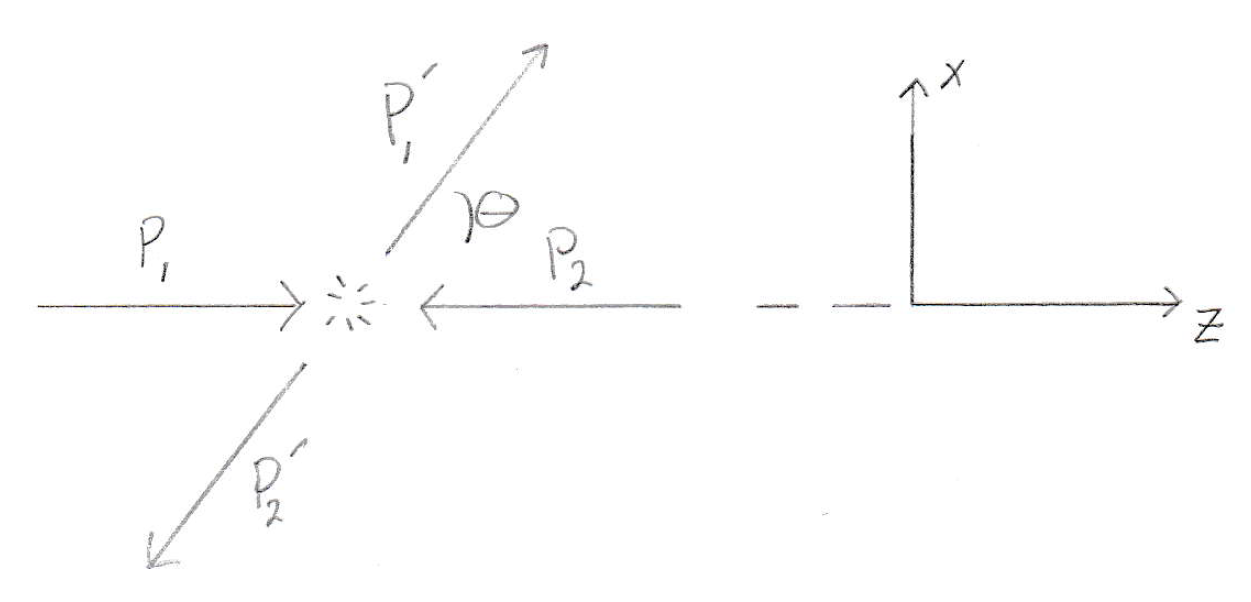
\includegraphics[width=0.8\textwidth]{figures/scat3}
	\caption{The kinematics of massive scattering.}
	\label{fig:shi}
\end{figure}
\begin{equation}
	p_1=\begin{bmatrix}
		E_1 \\ 0\\ 0 \\ p_{1z} \\
	\end{bmatrix} ,\quad
	p_2=\begin{bmatrix}
		E_2 \\ 0\\ 0\\ p_{2z}\\
	\end{bmatrix},\quad 
	p'_1=\begin{bmatrix}
		E'_1 \\ p'_{1x}\\ 0 \\ p'_{1z} \\
	\end{bmatrix} \quad \text{and}\quad
	p'_2=\begin{bmatrix}
		E'_2 \\ p'_{2x}\\ 0\\ p'_{2z}\\
	\end{bmatrix}.
\end{equation} 
In order to evaluate the three dimensional integrals in the phase space faction the delta function is split up as follows
\begin{equation}
	\delta^{(4)}(p_1+p_2-p'_1-p'_2)=\delta(E_1+E_2-E_1'-E'_2)\delta^{(3)}(\vec{p}_1+\vec{p}_2-\vec{p'}_1-\vec{p'}_2).
\end{equation} 
By using the three-dimensional delta-function the integral over $d^3p'_2$ becomes trivial and it is evaluated by setting $\vec{p'}_2=\vec{p}_1+\vec{p}_2-\vec{p'}_1=-\vec{p'}_1\Rightarrow E'_2=E'_2(p'_1)$. By using this
\begin{equation}
	\begin{split}
		\int d\Phi^{(2)}&=\int\frac{d^3p_1'}{(2\pi)^3}\frac{1}{2E_1 '}(2\pi)^4\delta(E_1+E_2-E_1'-E'_2)\int\frac{d^3p'_2}{(2\pi)^3}\frac{1}{2E'_2}\delta^{(3)}(\vec{p}_1+\vec{p}_2-\vec{p'}_1-\vec{p'}_2)\\
		&=\int\frac{d^3p_1'}{(2\pi)^3}\frac{(2\pi)\delta(E_1+E_2-E_1'-E'_2)}{4E'_1E_2'}.\\
	\end{split}
\end{equation} 
Next go to spherical coordinates such that $d^3p_1'\Rightarrow |\vec{p'}_1|^2d|\vec{p'}_1|d\Omega$. Hereby
\begin{equation}
	\begin{split}
		\int d\Phi^{(2)}&=\int\frac{d\Omega}{4(2\pi)^2}   \int\frac{|\vec{p'}_1|^2d|\vec{p'}_1|}{E'_1E'_2}\delta(E_1+E_2-E'-E_2').
	\end{split}
\end{equation} 
In order to evaluate the integral the delta function is rewritten by using that $\delta(f(x))=\frac{\delta(x-x_0)}{|\frac{df(x)}{dx}|}$, where $x_0$ is the zero\footnote{If there are more than one zero there should be a sum.} of $f(x)$. By using this identity
\begin{equation}
	\delta(E_1+E_2-E'_1-E_2')=\delta(|\vec{p'}_1|-p_0')\frac{1}{|\vec{p'}_1|\big(\frac{1}{E'_1}+\frac{1}{E'_2}\big)},
\end{equation} 
where is the value of $|\vec{p'}_1|$ that fulfills $E_1+E_2-E'_1(|\vec{p'}_1|)-E_2'(|\vec{p'}_1|)=0$. This defines the on-shell value of $|\vec{p'}_1|$. By using the delta function
\begin{equation}
	\begin{split}
		\int d\Phi^{(2)}&=\int\frac{d\Omega}{16\pi^2}   \frac{p_0'}{E'_1+E'_2}.
		\end{split}
	\label{eq2}
\end{equation} 
By using equation \eqref{eq2} and \eqref{obs} the differential cross section can, in the CM rest frame, be written as
\begin{equation}
	\frac{d\sigma}{d\Omega}=\frac{S}{4F}\frac{1}{16\pi^2}   \frac{p_0'}{E'_1+E'_2}\braket{|\mathcal{M}|^2}.
	\label{shiess}
\end{equation} 
For a $2\Rightarrow 2$ scattering in the CM rest frame the flux factor can be written as
\begin{equation}
	\begin{split}
		F&\equiv E_1E_2|\vec{v}_1-\vec{v}_2|\\
		&=\sqrt{(p_1\cdot p_2)^2-m_1^2m_2^2}\\
		&=\sqrt{E_1^2E_2^2+2E_1E_2|\vec{p}_1||\vec{p}_2|+|\vec{p}_1|^2|\vec{p}_2|^2-m_1^2m_2^2}\\
		&=|\vec{p}_1|\sqrt{\frac{(|\vec{p}_1|^2+m_1^2)(|\vec{p}_1|^2+m_2^2)}{|\vec{p}_1|^2}+2E_1E_2+|\vec{p}_1|^2-\frac{m_1^2m_2^2}{|\vec{p}_1|^2}}\\
		&=|\vec{p}_1|(E_1+E_2)\\
		&=|\vec{p}_1|(E'_1+E'_2),
	\end{split}
\end{equation} 
where both energy and momentum conservation for the CM rest frame has been used. By using the expression of the flux factor in the differential cross section
\begin{equation}
	\frac{d\sigma}{d\Omega}=\frac{S}{64\pi^2}   \frac{\braket{|\mathcal{M}|^2}}{(E'_1+E'_2)^2}\frac{|\vec{p'}_1|}{|\vec{p}_1|}.
	\label{diffcrossmass}
\end{equation} 
The total cross section is then found by integrating over the solid angle. To this end the invariant amplitude must however be known since it can depend on the solid angle.

\section{Massless scattering}
\index{Kinematics of massless scattering}
The phase space factor under consideration is given by equation \eqref{kin1}. Considering the scattering event from the reference frame in which the massive particle is initially at rest, the respective coordinates can, cf. figure \ref{fig:11}, be described as
\begin{figure}[H]
	\captionsetup{width=1\textwidth}
	\centering
	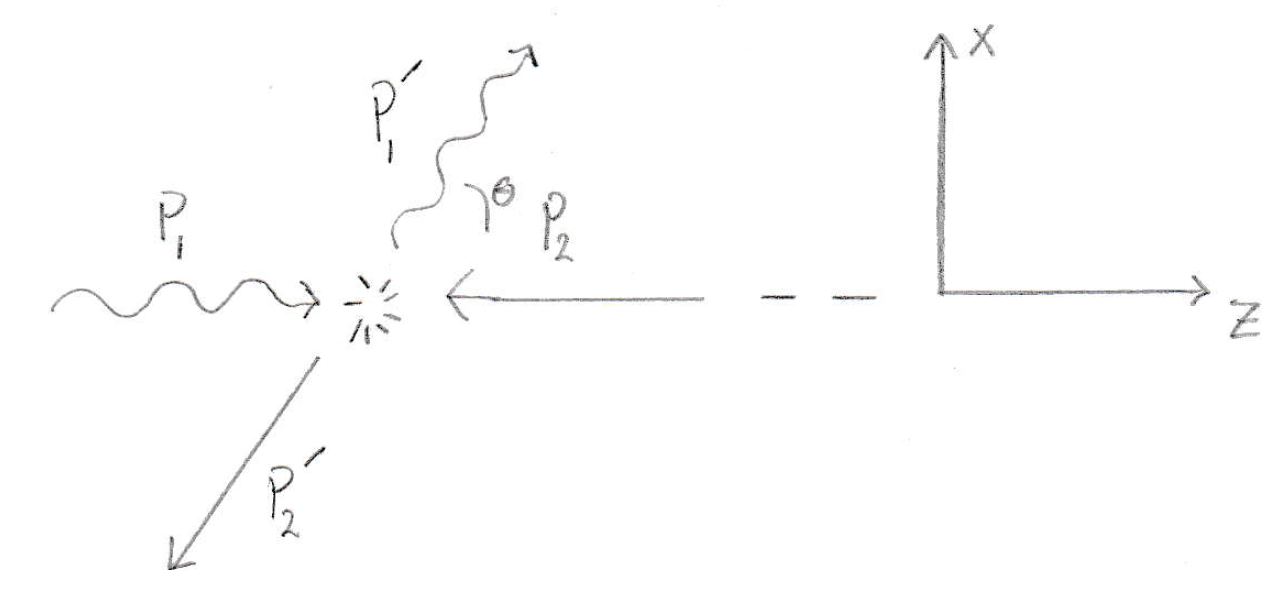
\includegraphics[width=0.8\textwidth]{figures/scat4}
	\caption{The kinematics of massless scattering.}
	\label{fig:11}
\end{figure}
\begin{equation}
	p_1=\begin{bmatrix}
		E_1 \\ 0\\ 0 \\ |\vec{p}_1| \\
	\end{bmatrix} ,\quad
	p_2=\begin{bmatrix}
		E_2 \\ -\vec{p}_1\\
	\end{bmatrix},\quad 
	p'_1=\begin{bmatrix}
		E'_1 \\ |\vec{p'}_1| \sin(\theta)\\ 0 \\ |\vec{p'}_1|\cos(\theta) \\
	\end{bmatrix} \quad \text{and}\quad
	p'_2=\begin{bmatrix}
		E'_2 \\ -\vec{p'}_1\\
	\end{bmatrix}, 
\end{equation} 
where $E_1=|\vec{p}_1|$ and $E'_1=|\vec{p'}_1|$.	As compared to the massive case, the massless case differs by the kinematics and the flux factor. The flux factor in the massless case is $F=\sqrt{(p_1\cdot p_2)^2-m_1^2m_2^2}=E_1 (E_2+E_1)=E_1E_{CM}=|\vec{p}_1|E_{CM}$ , where $E_{CM}\equiv E_1+E_2=E'_1+E'_2$. By using this in equation \eqref{shiess}
\begin{equation}
	\begin{split}
		\frac{d\sigma}{d\Omega}&=\frac{S}{4|\vec{p}_1| E_{CM}}\frac{1}{16\pi^2}   \frac{|\vec{p'}_1|}{E_{CM}}\braket{|\mathcal{M}|^2}\\
		&=\frac{S}{64\pi^2E_{CM}^2}   \frac{|\vec{p'}_1|}{|\vec{p}_1|}\braket{|\mathcal{M}|^2}.\\
	\end{split}
	\label{diffcrossmass1}
\end{equation} 

\section{$1\Rightarrow 2$ decay}
\index{Kinematics of $1\Rightarrow 2$ decay}
The phase space factor for $1\Rightarrow 2$ decay is given by
\begin{equation}
	\int d\Phi^{(2)}=\int\frac{d^3p'_1}{(2\pi)^3}\int\frac{d^3p'_2}{(2\pi)^3}\frac{(2\pi)^4\delta^{(4)}(p-p'_1-p_2')}{4E'_{1}E'_{2}}.
\end{equation} 
Considering the scattering event from the frame in which the initial particle is at rest, the respective coordinates can, cf. figure \ref{fig:21}, be described as
\begin{figure}[H]
	\captionsetup{width=1\textwidth}
	\centering
	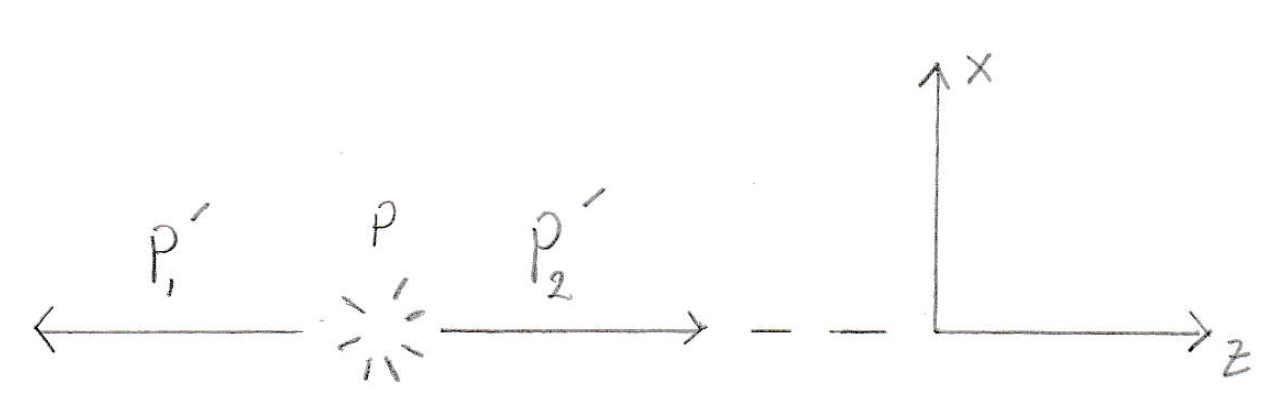
\includegraphics[width=0.8\textwidth]{figures/scat5}
	\caption{The kinematics of the decay.}
	\label{fig:21}
\end{figure}
\begin{equation}
	p=\begin{bmatrix}
		m \\ \vec{0}\\
	\end{bmatrix}, \quad 
	p_1'=\begin{bmatrix}
		E'_1 \\ \vec{p'}_1\\
	\end{bmatrix} \quad \text{and}\quad
	p_2'=\begin{bmatrix}
		E'_2 \\ \vec{p'}_2\\
	\end{bmatrix},
\end{equation}  
where from conservation of momentum, $k=q+p$
\begin{equation}
	\begin{bmatrix}
		m \\ \vec{0} \\
	\end{bmatrix}= \begin{bmatrix}
	E'_1+E'_2 \\ \vec{p'}_1+\vec{p'}_2\\
\end{bmatrix}.
\end{equation} 
Splitting the delta function
\begin{equation}
	\delta^{(4)}(p-p'_1-p'_2)=\delta(m-E'_1-E'_2)\delta^{(3)}(\vec{p'}_1+\vec{p'}_2).
\end{equation} 
From this the integration over $d^3p'_2$ can be eliminated, setting $\vec{p'}_1=-\vec{p'}_2$
\begin{equation}
	\begin{split}
		\int d\Phi^{(2)}&=\int\frac{d^3p'_1}{(2\pi)^3}\frac{(2\pi)\delta(m-E'_1-E'_2)}{4E'_{1}E'_{2}}\\
		&=\int \frac{d\Omega}{16\pi^2}\int \frac{|\vec{p'}_1|^2d|\vec{p'}_1|}{E'_{1}E'_{2}}\delta(m-E'_1-E'_2).\\
	\end{split}
	\label{int2}
\end{equation} 
To evaluate the integral the delta function must be rewritten in terms of the integration variable. Using that, because of the first integral, $E'_1=E_1'(|\vec{p'}_1|), E'_2=E_2'(|\vec{p'}_1|)$. By applying the same procedure as in the previous cases
\begin{equation}
	\delta(m-E'_1-E'_2)=\frac{E_1'}{|\vec{p'}_1|}\delta(|\vec{p'}_1|-p_0).
\end{equation} 
By using this in equation \ref{int2}
\begin{equation}
	\begin{split}
		\int d\Phi^{(2)}&=\int \frac{d\Omega}{16\pi^2}\int \frac{|\vec{p'}_1|d|\vec{p'}_1|}{E'_{2}}\delta(|\vec{p'}_1|-p_0)\\
		&=\int \frac{d\Omega}{16\pi^2}\frac{p_0}{E'_{2}}.\\
	\end{split}
	\label{int3}
\end{equation} 
By using equation \eqref{int3} alongside equation \eqref{obs}
\begin{equation}
	\frac{d\Gamma}{d\Omega}=\frac{S}{32\pi^2m}\frac{|\vec{p'}_1|}{E'_{2}}\braket{|\mathcal{M}|^2},
\end{equation} 
where it once more has been used that $p_0$ is the on-shell value of $|\vec{p'}_1|$ and so $p_0=|\vec{p'}_1|$ has been used in the end.

\section{The Invariant Matrix Element}
The invariant matrix element is defined in terms of the transition amplitude between two states. The amplitude is given by
\begin{equation}
	\mathcal{A}\equiv \braket{f|S|i},
	\label{S1}
\end{equation} 
where $S$ is the operator, called the scattering operator, evolving the initial state to the final state and
\begin{equation}
	\begin{split}
		&\ket{i}=\ket{\vec{p}_1}\otimes \ket{\vec{p}_2}\otimes \dots =\bigotimes_{i}\,\ket{\vec{p}_i}\\
		&\bra{f}=\dots \otimes \bra{\vec{p'}_2}\otimes \bra{\vec{p'}_1}=\bra{\vec{p'}_j}\bigotimes_j.
	\end{split}
\end{equation} 
For future reference I will use $p$ as initial momenta and $p'$ as final momenta. If $S=1$ there are no scattering between the particles and $\mathcal{A}$ is only non-vanishing if the initial and final state are equal. Motivated by this the $S$-operator is defined in terms of a non-interacting ($1$) and interacting ($T$) part cf.
\begin{equation}
	S\equiv 1+iT.
	\label{S2}
\end{equation} 
Using this definition in $\mathcal{A}$ leads to the definition of the invariant matrix element. $\mathcal{A}$ in terms of $T$ is given by
\begin{equation}
	\mathcal{A}=\braket{f|i}+\braket{f|iT|i}.
	\label{S3}
\end{equation} 
The $T$-part always carry a delta function securing momentum conservation at the vertexes. This is by convention factored from the last term alongside a factor of $(2\pi)^4$. Hereby
\begin{equation}
	\begin{split}
		\mathcal{A}&=\braket{f|i}+(2\pi)^4\delta^{(4)}(\Sigma p'-\Sigma p)\underbrace{\frac{\braket{f|iT|i}}{(2\pi)^4\delta^{(4)}(\Sigma p'-\Sigma p)}}_{\equiv i\mathcal{M}}\\
		&=\braket{f|i}+(2\pi)^4\delta^{(4)}(\Sigma p'-\Sigma p)i\mathcal{M}.
	\end{split}
	\label{S4}
\end{equation} 
So, the invariant matrix element is defined from the interactive part of a transition amplitude. The invariant matrix element is most often calculated from Feynman diagrams and Feynman rules.  However, it can also be done by a more rigorous procedure - the one used before Feynman diagrams; by relating $\mathcal{M}$ to the n-point functions of the theory. The relationship between the invariant matrix element and the n-point functions depend on the theory, and so in order to illustrate the relationship I have to pick a theory. To keep it simple I will consider an interactive scalar theory, eg. $\phi^4$-theory. The formula I am looking for, relation the invariant matrix element to the n-point functions of the theory, is called the LSZ reduction formula.

\subsection*{The LSZ Reduction Formula}
Consider the transition amplitude
\begin{equation}
	\mathcal{A}=\underbrace{\braket{f|S|i}}_{\text{Schroedinger scheme}}=\underbrace{\braket{f,t_f|S|i,t_i}}_{\text{Heisenberg scheme}}.
\end{equation} 
Since the goal is to relate the invariant matrix element to the n-point functions (which are on the form $\braket{\Omega|T\{\dots\}|\Omega}$), it is desired to somehow to "remove" the particles from the states and represent them by fields in between the states. Particles can be "pulled" from states by using that $\ket{\vec{p}}=\sqrt{2E_{\vec{p}}}a_{\vec{p}}^\dagger\ket{0}$. The ladder operators are then related to the fields, so intuitively the idea seems reasonable. For a \emph{free} theory the field can be expressed in terms of the mode expansion. This expression can be inverted to isolate the ladder operators to find
\begin{equation}
	\sqrt{2E_{\vec{p}}}\,a_{\vec{p}}=i\int d^3x e^{ip\cdot x}\overleftrightarrow{\partial}_0\phi_{free}, \quad \sqrt{2E_{\vec{p}}}\,a_{\vec{p}}^\dagger=-i\int d^3x e^{-ip\cdot x}\overleftrightarrow{\partial}_0\phi_{free},
\end{equation} 
where
\begin{equation}
	e^{ip\cdot x} \overleftrightarrow{\partial}_0\phi_{free}=e^{ip\cdot x}\partial_0\phi_{free}-\phi_{free}\partial_0e^{ip\cdot x}.
\end{equation} 
However, the fields under consideration are not free - they are interactive (recall the $\phi^4$-statement). However, interactive fields cannot be expanded in the mode expansion, so it is desired to relate the free fields to the interactive fields. To this end assume that infinitely far away in time, before and after the scattering, the fields are free. This assumption is reasonable for weakly interacting theories, but not in general - for example it is not reasonable for QCD. So, taking the theory under consideration to be weakly interacting
\begin{equation}
	\phi\xrightarrow{t\Rightarrow \pm\infty}\sqrt{Z}\phi_{out/in},
\end{equation} 
where $Z$ is the wave function renormalization factor and $\phi_{out/in}$ are free fields infinitely before and after in time. From these definitions
\begin{equation}
	\sqrt{2E_{\vec{p}}}\,a_{\vec{p}}^{in \dagger}=-iZ^{-\frac{1}{2}}\lim_{t\Rightarrow -\infty}\bigg(\int d^3x e^{-ip\cdot x}\overleftrightarrow{\partial}_0\phi\bigg),
\end{equation} 
where the field on the RHS is the field of the full theory, i.e. not the free field. From this definition one of the particles of the initial state can be "pulled" from the initial state via.
\begin{equation}
	\begin{split}
		\mathcal{A}&=\sqrt{2E_{\vec{p}_1}}\,\braket{\Sigma\vec{p'},t_f|a_{\vec{p}_1}^{in \dagger}|\Sigma\vec{p}-\vec{p}_1,t_i}\\
		&=-iZ^{-\frac{1}{2}}\lim_{t\Rightarrow -\infty}\bigg(\int d^3x e^{-ip_1\cdot x}\braket{\Sigma\vec{p'},t_f|\overleftrightarrow{\partial}_0\phi|\Sigma\vec{p}-\vec{p}_1,t_i}\bigg).\\
	\end{split}
\end{equation} 
It is desired to get rid of the limit in the above expression. In order to do this use the identity
\begin{equation}
	\bigg( \lim_{t\Rightarrow \infty} -\lim_{t\Rightarrow -\infty} \bigg)\int d^3x f(\vec{x},t)=\int_{-\infty}^{\infty}dt \frac{d}{dt}\bigg(\int d^3x f(\vec{x},t)\bigg).
\end{equation} 
To use this identity, the "subtracted limit" is needed. To get this, assume that there are no spectating particles - i.e. no particles that does not interact. If this is the case, then $\bra{\Sigma \vec{p'}}a_{\vec{p}}^{out\dagger}=0$. Since one can always add zero, the transition amplitude can be written as
\begin{equation}
	\mathcal{A}=\sqrt{2E_{\vec{p}_1}}\,\braket{\Sigma\vec{p'},t_f|(a_{\vec{p}_1}^{in \dagger}-a_{\vec{p_1}}^{out\dagger})|\Sigma\vec{p}-\vec{p}_1,t_i}.\\
\end{equation} 
By expressing $\sqrt{2E_{\vec{p}_1}}\,a_{\vec{p_1}}^{out\dagger}$ in terms of the field the identity can be used. Take $f(\vec{x},t)\rightleftarrows -iZ^{-\frac{1}{2}}e^{-ip_1\cdot x}\overleftrightarrow{\partial}_0\phi$. By using the identity, and swapping the time-derivative and integration over $d^3x$
\begin{equation}
	\sqrt{2E_{\vec{p}_1}}\,(a_{\vec{p}_1}^{in \dagger}-a_{\vec{p_1}}^{out\dagger})=iZ^{-\frac{1}{2}}\int d^4x \partial_0(e^{-ip_1\cdot x}\overleftrightarrow{\partial}_0\phi),
\end{equation} 
where the positive sign comes from the fact that $a_{\vec{p}_1}^{in \dagger}-a_{\vec{p_1}}^{out\dagger}\propto\lim_{t\Rightarrow -\infty} -\lim_{t\Rightarrow \infty}$. Applying the time derivatives and writing it out
 \begin{equation}
	\begin{split}
		\sqrt{2E_{\vec{p}_1}}\,(a_{\vec{p}_1}^{in \dagger}-a_{\vec{p_1}}^{out\dagger})&=iZ^{-\frac{1}{2}}\int d^4x \partial_0(e^{-ip_1\cdot x}\overleftrightarrow{\partial}_0\phi)\\
		&=iZ^{-\frac{1}{2}}\int d^4x \partial_0(e^{-ip_1\cdot x}\partial_0\phi+iE_{\vec{p}_1}e^{-ip_1\cdot x}\phi)\\
		&=iZ^{-\frac{1}{2}}\int d^4x (-iE_{\vec{p}_1}e^{-ip_1\cdot x}\phi+e^{-ip_1\cdot x}\partial_0^2\phi+E_{\vec{p}_1}^2e^{-ip_1\cdot x}\phi+iE_{\vec{p}_1}e^{-ip_1\cdot x}\phi) \\
		&=iZ^{-\frac{1}{2}}\int d^4x e^{-ip_1\cdot x}(\partial_0^2+E_{\vec{p}_1}^2)\phi \\
		&=iZ^{-\frac{1}{2}}\int d^4x e^{-ip_1\cdot x}(\partial_0^2+m_{\vec{p}_1}^2+(\vec{p}_1)^2)\phi \\
		&=iZ^{-\frac{1}{2}}\int d^4x (e^{-ip_1\cdot x}\partial_0^2\phi+\phi(m_{\vec{p}_1}^2-\nabla^2)e^{-ip_1\cdot x})\\
		&=iZ^{-\frac{1}{2}}\int d^4x (e^{-ip_1\cdot x}(\square_x+m_{\vec{p}_1}^2)\phi,\\
	\end{split}
\end{equation} 
where integration by parts has been used twice to shift $\nabla^2$ from the exponential to $\phi$. From using the above the transition amplitude is given by
\begin{equation}
	\mathcal{A}=iZ^{-\frac{1}{2}}\int d^4x e^{-ip_1\cdot x}(\square _x+m_{\vec{p}_1}^2)\braket{\Sigma\vec{p'},t_f|\phi(x)|\Sigma\vec{p}-\vec{p}_1,t_i}.
\end{equation} 
By continuing this way all particles from the initial and final states can be removed and represented by fields instead. Denoting the "position belonging to the final-state particles" by $y$ and the "position belonging to the initial-state particles" by $x$ the transition amplitude can therefore be written as
\begin{equation}
	\begin{split}
		\mathcal{A}&=\bigg(i\frac{1}{\sqrt{Z}}\bigg)^{n+m}\int\prod_{i=1}^m d^4x_i\int\prod_{j=1}^n d^4y_ie^{i(p'_j\cdot y_j-p_i\cdot x_i)}(\square _{x_i}+m_{\vec{p}_i}^2)(\square _{y_j}+m_{\vec{p'}_j}^2)\\
		&\quad\cdot\braket{\Omega|T\{\phi(x_1)\dots\phi(x_m)\phi(y_1)\dots \phi(y_n)\}|\Omega}.\\
	\end{split}
	\label{am}
\end{equation} 
However, since no spectating particles has been assumed, equation \eqref{am} only denotes the interactive part of the transition amplitude. Therefore
\begin{equation}
	\begin{split}
		\braket{f|iT|i}&=\bigg(i\frac{1}{\sqrt{Z}}\bigg)^{n+m}\int\prod_{i=1}^m d^4x_i\int\prod_{j=1}^n d^4y_ie^{i(p'_j\cdot y_j-p_i\cdot x_i)}(\square _{x_i}+m_{\vec{p}_i}^2)(\square _{y_j}+m_{\vec{p'}_j}^2)\\
		&\quad\cdot\braket{\Omega|T\{\phi(x_1)\dots\phi(x_m)\phi(y_1)\dots \phi(y_n)\}|\Omega}.\\
	\end{split}
	\label{am1}
\end{equation} 
Equation \eqref{am1} is a version of the so-called LSZ formula which relates the interactive part of the transition amplitude to the n-point functions of the interactive theory. Similar expressions can be obtained for fermion or boson fields by repeating a similar procedure. The result will be a similar expression with different fields, a possible minus sign (due to anti-commutation of fermion fields) and the Dirac operator instead of the KG operator. Note that $\phi(x)$ is not a free field, but a field of the entire field. This is the reason why $(\square +m^2)\phi\neq0$, i.e. the KG equation is only valid for free fields. 

\subsection*{Perturbation theory in QFT}
After having related the n-point functions for the interactive theory to the invariant matrix element it is time to determine the n-point functions themselves. Recall that an interactive theory is considered, so for example the two-point function is not the propagator. This is only the case for a free theory - i.e. a non-interactive theory. What is desired is to relate the n-point functions of the interactive theory to the n-point functions of the free theories, i.e. relate the interactive fields to the free fields and the interactive vacuum state to the free vacuum state. To this end use what is called the interaction scheme of QM. In this scheme both the states and operators are time-dependent cf.
\begin{equation}
	\ket{\psi_I(t)}\equiv e^{iH_0t}\ket{\psi_S(t)},\quad A_I(t)\equiv e^{iH_0t}A_Se^{-iH_0t},
\end{equation} 
where $I$ denotes the interaction scheme, $S$ denotes the Schroedinger scheme and $H_0$ is the free part of an interactive Hamiltonian. The interactive theory is characterized by a Lagrangian density on the form
\begin{equation}
	\mathcal{L}=\mathcal{L}_{0}+\mathcal{L}_{int},
	\label{lag}
\end{equation} 
where $\mathcal{L}_{0}=\mathcal{L}_{free}$. Equation \eqref{lag} is true for all theories, not only scalar field theories. The Lagrangian density corresponds to a Hamiltonian density on the form
\begin{equation}
	\mathcal{H}=\mathcal{H}_{0}+\mathcal{H}_{int}.
\end{equation} 
The solution to the EOM's for the interactive theory is in general very difficult (at best) to obtain. Since the theory is not free it is however clear that the field will not be given in terms of a simple mode expansions. However, the interactive field can bed related to the free field by using the interaction scheme. Since the free field in the mode expansion is represented in the Heisenberg scheme, and $A_H(t)=e^{iHt}A_Se^{-iHt}$, the interactive field can be related to the free field in the interactive scheme via.
\begin{equation}
	\phi(x)=U^\dagger(t,t_0)\phi_I(x)U(t,t_0),
\end{equation} 
where\footnote{Note that $[H_{0},H]\neq 0$ in general so the exponentials cannot be "collected".} $U(t,t_0)=e^{iH_0(t-t_0)}e^{-iH(t-t_0)}$ is the time-evolution operator and $\phi_I(x)$, the field in the interactive scheme, is a free field so it can be written in terms of the mode expansion,  i.e.
\begin{equation}
	\phi_I(x)=\int \frac{d^3 p}{(2\pi)^3}\frac{1}{\sqrt{2E_{\vec{p}}}}\bigg(a_{\vec{p}}\,e^{-ip\cdot x}+a_{\vec{p}}^*\,e^{ip\cdot x}\bigg)=\text{free field}.
\end{equation} 
The time-evolution operator, $U$, obeys the Schroedinger equation in the interaction picture. This can be seen by
\begin{equation}
	i\frac{\partial U(t,t_0)}{\partial t}=e^{iH_0(t-t_0)}(H-H_0)e^{-H(t-t_0)}=\underbrace{e^{iH_0(t-t_0)}H_{int}e^{-iH_0(t-t_0)}}_{\equiv H_I}U(t,t_0),
\end{equation} 
where $H_I=H_I(t)$ is the interaction Hamiltonian in the interaction picture. The Schroedinger equation can be solved to find
\begin{equation}
	U(t,t_0)=T\{e^{-i\int d^4x \mathcal{H}_I}\}\Rightarrow S\equiv T\{e^{-i\int_{-\infty}^{\infty} d^4x \mathcal{H}_I}\}.
	\label{S}
\end{equation} 
With the time-evolution operator in the interaction scheme expressed, and the interactive field expressed in terms of free fields and the time-evolution operator in the interaction scheme, I have related the interactive fields to the free fields - as I wanted. Next up is the relationship between the vacuum state of the interactive theory and the vacuum state of the free theory. In order to relate the two I consider
\begin{equation}
	\begin{split}
		e^{-iHt}\ket{0}&=\sum_n
		e^{-iHt}\ket{n}\braket{n|0}\\
		&=e^{-iE_0t}\ket{\Omega}\braket{\Omega|0}+\sum_{n\neq \Omega}e^{-iHt}\ket{n}\braket{n|0},\\
	\end{split}
\end{equation} 
where $\ket{n}$ are eigenstates of the full theory and $E_0<e_{n\neq 0}$. To get "rid" of the second term, employ a mathematical trick; let $t\Rightarrow T\Rightarrow \infty (1-i\varepsilon)$ - where $T$ just denotes complex time. Because $E_0<e_{n\neq 0}$ the $E_0$ term will die out last. Therefore, in the limit of $T\Rightarrow \infty (1-i\varepsilon)$
\begin{equation}
	\ket{\Omega}=\lim\limits_{T\Rightarrow \infty (1-i\varepsilon)}\bigg(\frac{e^{iHT}\ket{0}}{e^{-iE_0T}\braket{\Omega|0}}\bigg).
\end{equation} 
Since $T$ is taken in the limit of going to infinity, a small shift, $T\Rightarrow T+t_0$ makes no difference. Hereby
\begin{equation}
	\ket{\Omega}=\lim\limits_{T\Rightarrow \infty (1-i\varepsilon)}\bigg(\frac{e^{iH(T+t_0)}\ket{0}}{e^{-iE_0(T+t_0)}\braket{\Omega|0}}\bigg).
\end{equation} 
Use now that, since $H_0\ket{0}=0$
\begin{equation}
	e^{iH_0(T+t_0)}\ket{0}=(1-iH_0(T+t_0))\ket{0}=\ket{0}.
\end{equation} 
Hence, the vacuum state in the interactive theory can be written as
\begin{equation}
	\begin{split}
		\ket{\Omega}&=\lim\limits_{T\Rightarrow \infty (1-i\varepsilon)}\bigg(\frac{e^{iH(T+t_0)}e^{iH_0(T+t_0)}\ket{0}}{e^{-iE_0(T+t_0)}\braket{\Omega|0}}\bigg)\\
		&=\lim\limits_{T\Rightarrow \infty (1-i\varepsilon)}\bigg(\frac{U(t_0,T)\ket{0}}{e^{-iE_0(T+t_0)}\braket{\Omega|0}}\bigg).\\
	\end{split}
	\label{vacs}
\end{equation} 
By using equation \eqref{vacs} and the expression for $\phi$ in terms of $\phi_I$
\begin{equation}
	\braket{\Omega|T\{\phi(x_1)\dots \phi(x_N)\}|\Omega}=\lim\limits_{T\Rightarrow \infty (1-i\varepsilon)}\bigg(\frac{\braket{0|U^\dagger(t_0,T)[U(t_0,t)\phi_I(x_1)U(t,t_0)]\dots U(t_0,-T)|0}}{e^{-iE_0(2T)}|\braket{\Omega|0}|^2}\bigg).
\end{equation} 
To get rid of the denominator, I divide by
\begin{equation}
	1=\braket{\Omega|\Omega}=\frac{\braket{0|U(T,t_0)U(t_0,-T)|0}}{e^{-iE_0(2T)}|\braket{\Omega|0}|^2}.
\end{equation} 
Next collect the fields in the nominator under a time-ordering. By doing so the time-evolution operators can be collected to the exponential. Hereby the n-point function can be written as
\begin{equation}
	\braket{\Omega|T\{\phi(x_1)\dots \phi(x_N)\}|\Omega}=\lim\limits_{T\Rightarrow \infty (1-i\varepsilon)}\bigg(\frac{\braket{0|T\{\phi_I(x_1)\dots\phi_I(x_N)e^{-i\int d^4x \mathcal{H}_I}\}|0}}{\braket{0|T\{e^{-i\int d^4x \mathcal{H}_I}\}|0}}\bigg).
	\label{pert}
\end{equation} 
The last step is then to expand the exponential in a Taylor series and use $\mathcal{H}_I$ from th interactive theory. $\mathcal{H}_I$ can be found from
\begin{equation}
	\mathcal{H}_I=e^{iH_0(t-t_0)}\mathcal{H}_{int}e^{-iH_0(t-t_0)}=\mathcal{H}_{int}(\phi_I).
\end{equation} 
Hence, $\mathcal{H}_I$ is the interactive part of the Hamiltonian density with $\phi\Rightarrow \phi_I=\text{free field}$. Collecting the results of equation \eqref{S4}, \eqref{am1} and \eqref{pert}
\begin{equation}
	\begin{split}
		i\mathcal{M}&=\frac{\braket{f|iT|i}}{(2\pi)^4\delta^{(4)}(\Sigma p'-\Sigma p)}\\
		&=\frac{\big(i\frac{1}{\sqrt{Z}}\big)^{n+m}}{(2\pi)^4\delta^{(4)}(\Sigma p'-\Sigma p)}\int\prod_{i=1}^m d^4x_i\int\prod_{j=1}^n d^4y_ie^{i(p'_j\cdot y_j-p_i\cdot x_i)}(\square _{x_i}+m_{\vec{p}_i}^2)(\square _{y_j}+m_{\vec{p'}_j}^2)\\
		&\qquad \cdot\braket{\Omega|T\{\phi(x_1)\dots\phi(x_m)\phi(y_1)\dots \phi(y_n)\}|\Omega}\\
		&=\frac{\big(i\frac{1}{\sqrt{Z}}\big)^{n+m}}{(2\pi)^4\delta^{(4)}(\Sigma p'-\Sigma p)}\int\prod_{i=1}^m d^4x_i\int\prod_{j=1}^n d^4y_ie^{i(p'_j\cdot y_j-p_i\cdot x_i)}(\square _{x_i}+m_{\vec{p}_i}^2)(\square _{y_j}+m_{\vec{p'}_j}^2)\\
		&\qquad\cdot \lim\limits_{T\Rightarrow \infty (1-i\varepsilon)}\bigg(\frac{\braket{0|T\{\phi_I(x_1)\dots\phi_I(y_n)e^{-i\int d^4x \mathcal{H}_I}\}|0}}{\braket{0|T\{e^{-i\int d^4x \mathcal{H}_I}\}|0}}\bigg). 
	\end{split}
	\label{qw}
\end{equation} 
Equation \eqref{qw} is valid for a generic scalar theory.

\begin{example}
	\emph{Consider a scattering amplitude for a process with two initial particles, with momenta $\vec{p}_1$ and $\vec{p}_2$, into two final particles, with momenta $\vec{p'}_1$ and $\vec{p'}_2$, in $\phi^4$-theory. Take the interactive part of the Hamiltonian density to be on the form}
	\begin{equation}
		\mathcal{H}_I=\frac{\lambda}{4!}\phi^4,
	\end{equation} 
	\emph{where $\phi=\phi_I$ in this example. The coupling, $\lambda$, defines the strength of the interaction. }
	\begin{enumerate}
		\item \emph{Draw the Feynman diagrams in position space. Compute the amplitude in the case in which there is no interactions, i.e. for $\lambda=0$, and motivate why there is no contribution as expected.}
		
		I begin by writing writing explicitly the LSZ formula, with the KG operators taken to the LHS and represented in momentum space, for $\phi^4$-theory
		\begin{equation}
			\begin{split}
				&\bigg(\prod_{i=1}^{2}\frac{i\sqrt{Z}}{p'_i-m^2}\bigg)\bigg(\prod_{j=1}^{2}\frac{i\sqrt{Z}}{p_j-m^2}\bigg)\braket{\vec{p'}_1\vec{p'}_2|iT|\vec{p}_1\vec{p}_2}=\int d^4x_1\int d^4x_2\int d^4x_3\int d^4x_4\\
				&\cdot e^{i(p'_1\cdot x_1+p'_2\cdot x_2-p_1\cdot x_3-p_2\cdot x_4)}\frac{\braket{0|T\{\phi(x_1)\phi(x_2)\phi(x_3)\phi(x_4)e^{-i\frac{\lambda}{4!}\int d^4x\phi^4}\}|0}}{\braket{0|T\{e^{-i\frac{\lambda}{4!}\int d^4x \phi^4}\}|0}}.
			\end{split}
		\end{equation}  
		I take the lowest non-trivial order in perturbation theory - Ie. I will work to $\mathcal{O}(\lambda)$. In this theory
		\begin{equation}
			Z=1+\mathcal{O}(\lambda^2).
		\end{equation} 
		Therefore, I take $Z=1$. I also expand the exponential cf.
		\begin{equation}
			e^{-i\frac{\lambda}{4!}\int d^4x \phi^4}=1-i\frac{\lambda}{4!}\int d^4x\phi^4+\mathcal{O}(\lambda^2).
		\end{equation} 
		To $\mathcal{O}(\lambda^0)$, with $Z=1$, I find from the LSZ formula
		\begin{equation}
			\begin{split}
				&\frac{i}{p'_1-m^2}\frac{i}{p'_2-m^2}\frac{i}{p_1-m^2}\frac{i}{p_2-m^2}\braket{\vec{p'}_1\vec{p'}_2|iT|\vec{p}_1\vec{p}_2}=\int d^4x_1\int d^4x_2\int d^4x_3\int d^4x_4\\
				&\cdot e^{i(p'_1\cdot x_1+p'_2\cdot x_2-p_1\cdot x_3-p_2\cdot x_4)}\braket{0|T\{\phi(x_1)\phi(x_2)\phi(x_3)\phi(x_4)\}|0}.
			\end{split}
		\end{equation}  
		The VEV is computed by using Wicks theorem\index{Wicks theorem}. Wicks theorem states that a time-ordered series of field-operators is related to the normal-ordered series of field-operators, via.
		\begin{equation}
			T\{\phi_1\phi_2\dots\phi_n\}=N\{\phi_1\phi_2\dots\phi_n+\text{All contractions}\}.
		\end{equation} 
		Wicks theorem is extremely useful when considering a VEV, because the normal ordered product of free field operators vanish\footnote{Because the normal-ordering operator acts to put the annihilation operators to eh right, they will act on the vacuum and make the term vanish.}. The only terms that does not vanish are the ones which are fully contracted. For the VEV under consideration
		\begin{equation}
			\begin{split}
				VEV&=\braket{0|T\{\phi_1\phi_2\phi_3\phi_4\}|0}\\
				&
				\contraction{,,,,,,,,,,,,,,,,,,,,}{\phi_1}{.}{\phi_2}
				\contraction{,,,,,,,.,,,,,,,,,,,,,,,,,,,,,,,,,}{\phi_1}{,,}{\phi_2}
				\contraction{,,,,,,,,,,,,,,,,,,,,,,.,,,,,,,,,,,,,,,,,,,,,,}{\phi_1}{,,,,}{\phi_2}
				\contraction{,,,,,,,,,,,,,,,,,,,,,,,,.,,,,,,,,,,,,,,,,,,,,,,,,,,,,,,,,,,}{\phi_1}{.}{\phi_2}
				=\braket{0|N\{\phi_1\phi_2\phi_3\phi_4+\phi_1\phi_2\phi_3\phi_4+\phi_1\phi_2\phi_3\phi_4+\phi_1\phi_2\phi_3\phi_4+\phi_1\phi_2\phi_3\phi_4}\\
					&{
					\contraction{,,,,,}{\phi_1}{,,}{\phi_2}
					\contraction{,,,,,,,,,,,.,.,,,,,,}{\phi_1}{.}{\phi_2}
					\contraction{,,,,,,,,,,,,,,,,,,,,,,,,,,}{\phi_1}{.}{\phi_2}
					\contraction{,,,,,,,,,,,,,,,,,,,,,,,,,,,,,,,}{\phi_1}{.}{\phi_2}
					\contraction[2ex]{,,,,,,,,,,,,,,,,,,,,,,,,,,,,,,,,,,,,,,}{\phi_1}{,,,}{\phi_2}
					\contraction{,,,,,,.,,,,,,,,,,,,,,,,,,,,,,,,,,,,,,,,,,}{\phi_1}{.,,}{\phi_2}
					\contraction[2ex]{,,,,,,,,,,,,,,,,,,,,,,,,,,,,,,,,,,,,,,,,,,,,,,,,,,}{\phi_1}{,,,,.,}{\phi_2}
					\contraction{,,,,,,.,,,,,,,,,,,,,,,,,,,,,,,,,,,,,,,,,,,,,,,,,,,,,,}{\phi_1}{.}{\phi_2}
					+\phi_1\phi_2\phi_3\phi_4+\phi_1\phi_2\phi_3\phi_4+\phi_1\phi_2\phi_3\phi_4+\phi_1\phi_2\phi_3\phi_4+\phi_1\phi_2\phi_3\phi_4\}|0}.\\
			\end{split}
		\end{equation} 
		Now use that the contractions are complex numbers and as such they can be moved outside the Normal-ordering operator and bracket. Hence, what remains, besides the contraction, for fully contracted terms is $\braket{0|N\{1\}|0}=1$. Hereby
		\begin{equation}
			\contraction{,,,,,,,,,,,,,.,,,,,,.,}{\phi_1}{.}{\phi_2}
			\contraction{,,,,,,,,,,,,,,.,,,,,,,,,,,}{\phi_1}{.}{\phi_2}
			\contraction[2ex]{,,,,,,,,,,,,,,,,,,,,,,,,,,,,,,,,,}{\phi_1}{,,,}{\phi_2}
			\contraction{,,,,,,.,,,,,,,,..,,,,,,,,,,,,,,,,,,,,}{\phi_1}{..,}{\phi_2}
			\contraction[2ex]{,,,,,,,,,,,,,,.,,,,,,,,,,,,,,,,,,,,,,,,,,,,,,,}{\phi_1}{,,,,.}{\phi_2}
			\contraction{,,,,,,.,,,,,,,,,,,,,,,,,,,,,,,,,,,,,,,,,,,,,,,,,}{\phi_1}{.}{\phi_2}
			\braket{0|T\{\phi_1\phi_2\phi_3\phi_4\}|0}=\phi_1\phi_2\phi_3\phi_4+\phi_1\phi_2\phi_3\phi_4+\phi_1\phi_2\phi_3\phi_4.
		\end{equation} 
		Defining now
		\begin{equation}
			\contraction{}{\phi_1}{,,}{\phi_2}
			\phi(x_i)\phi(x_j)\equiv D(x_i-x_j)=D_{ij}.
		\end{equation} 
		The VEV becomes
		\begin{equation}
			\braket{0|T\{\phi_1\phi_2\phi_3\phi_4\}|0}=D_{12}D_{34}+D_{13}D_{24}+D_{14}D_{23}.
		\end{equation} 
		The VEV can be represented by Feynman diagrams
		\begin{figure}[H]
			\captionsetup{width=1\textwidth}
			\centering
			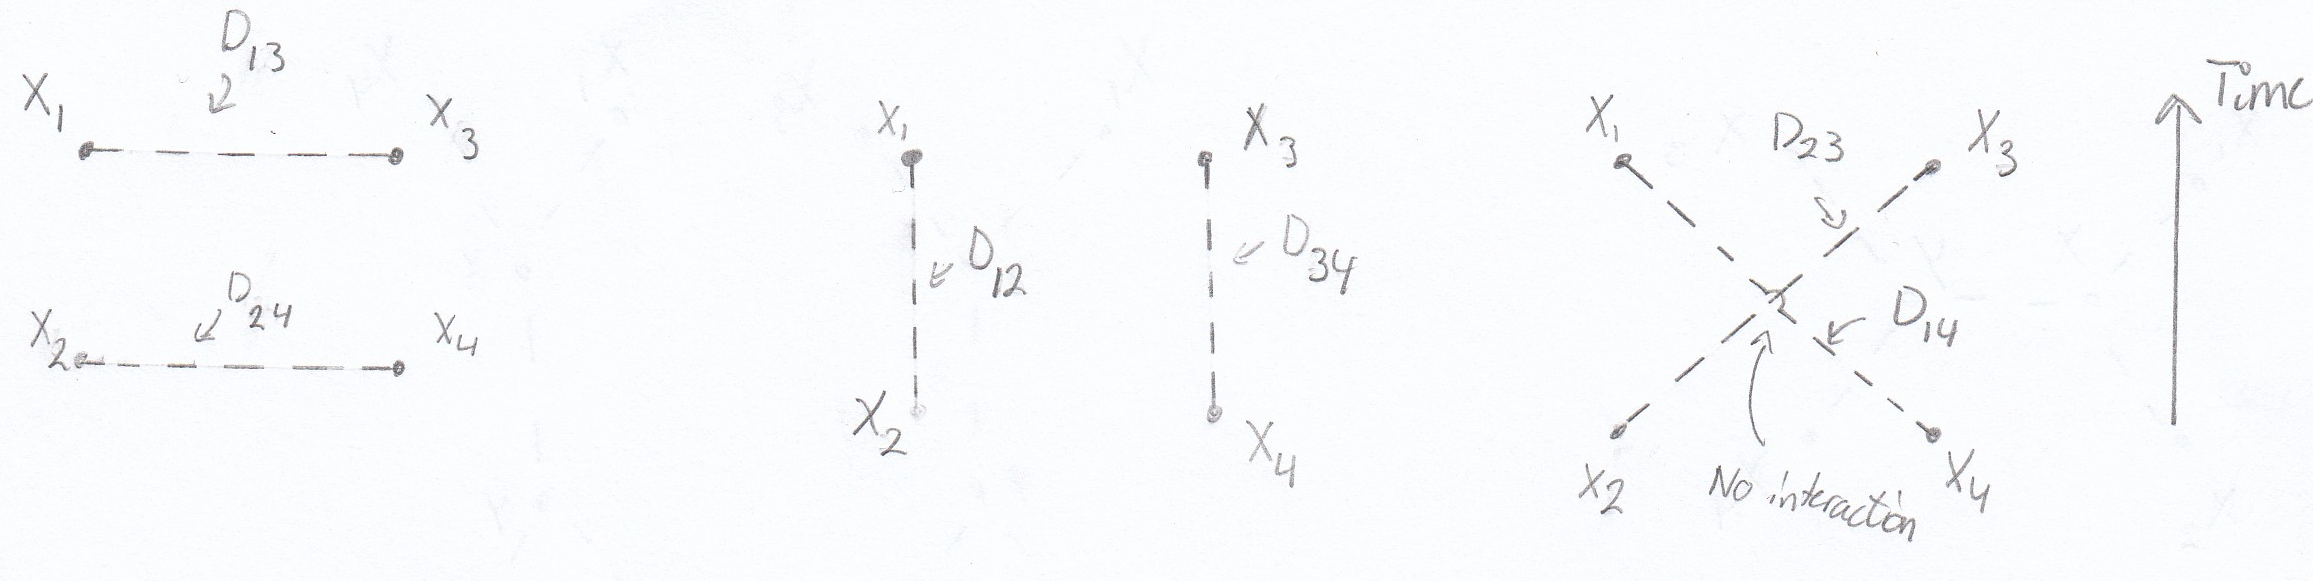
\includegraphics[width=0.9\textwidth]{figures/scal}
		\end{figure} 
		The diagrams show two particles traveling between two separate space-time-points without interacting. By using the expression for the VEV in the LSZ reduction formula to $\mathcal{O}(\lambda^0)$, with $z=1$, reveals
		\begin{equation}
			\begin{split}
				&\frac{i}{p'_1-m^2}\frac{i}{p'_2-m^2}\frac{i}{p_1-m^2}\frac{i}{p_2-m^2}\braket{\vec{p'}_1\vec{p'}_2|iT|\vec{p}_1\vec{p}_2}=\int d^4x_1\int d^4x_2\int d^4x_3\int d^4x_4\\
				&\cdot e^{i(p'_1\cdot x_1+p'_2\cdot x_2-p_1\cdot x_3-p_2\cdot x_4)}(D_{12}D_{34}+D_{13}D_{24}+D_{14}D_{23}).
			\end{split}
		\end{equation} 
		There are three integrals, of the propagators, to be evaluated. The first
		\begin{equation}
			I_1\equiv \int d^4x_1\int d^4x_2\int d^4x_3\int d^4x_4 e^{i(p'_1\cdot x_1+p'_2\cdot x_2-p_1\cdot x_3-p_2\cdot x_4)}D(x_1-x_2)D(x_3-x_4).
		\end{equation} 
		To evaluate $I_1$ I take $x'=x_1-x_2, x''=\frac{1}{2}(x_1+x_2),x'''=x_3-x_4,x''''=\frac{1}{2}(x_3+x_4)$. Hereby
		\begin{equation}
			\begin{split}
				I_1&\equiv \bigg(\underbrace{\int d^4x' \int d^4x''e^{i(p'_1+p'_2)x''}e^{\frac{i}{2}(p'_1-p'_2)x'}D(x')}_{\equiv I_4}\bigg)\\
				&\qquad\cdot\bigg(\underbrace{\int d^4x''' \int d^4x''''e^{-i(p_1+p_2)x''''}e^{-\frac{i}{2}(p_1-p_2)x'''}D(x''')}_{\equiv I_5}\bigg).\\
			\end{split}	
		\end{equation}  
		Now
		\begin{equation}
			\begin{split}
				I_4&=\int d^4x' \int d^4x''e^{i(p'_1+p'_2)x''}e^{\frac{i}{2}(p'_1-p'_2)x'}D(x')\\
				&=(2\pi)^4\delta^{(4)}(p'_1+p'_2)\int\frac{d^4p'}{(2\pi)^4}\frac{i}{p'^2-m^2}\underbrace{\int d^4x'e^{-i(p'-\frac{p'_1}{2}+\frac{p'_2}{2})\cdot x'}}_{=(2\pi)^4\delta^{(4)}(p'-\frac{p'_1}{2}+\frac{p'_2}{2})},
			\end{split}
		\end{equation} 
		where the propagator has been expressed in the momentum representation\footnote{Using $D(x_1-x_2)=\int\frac{d^4p'}{(2\pi)^4}\frac{i}{p'^2-m^2}e^{-ip'\cdot(x_1-x_2)}$.}. Now, use $\delta^{(4)}(p'_1+p'_2)\Rightarrow p_1'=-p_2'$ in $\delta^{(4)}(p'-\frac{p'_1}{2}+\frac{p'_2}{2})$. Hereby $\delta^{(4)}(p'-p_1')$. Hence, the integral can be killed off to reveal
		\begin{equation}
			I_4=\frac{(2\pi)^4}{p_1'^2-m^2}.
		\end{equation} 
		Likewise
		\begin{equation}
			\begin{split}
				I_5&=(2\pi)^4\delta^{(4)}(p_1+p_2)\int\frac{d^4p}{(2\pi)^4}\frac{i}{p^2-m^2}\underbrace{\int d^4x''''e^{-i(p+\frac{p_1}{2}-\frac{p_2}{2})\cdot x''''}}_{=(2\pi)^4\delta^{(4)}(p+\frac{p_1}{2}-\frac{p_2}{2})}.
			\end{split}
		\end{equation} 
		Repeating the procedure results in $k_1=-k_2\Rightarrow \delta^{(4)}(p+\frac{p_1}{2}-\frac{p_2}{2})=\delta^{(4)}(p+p_1)$. Hence, the integral will let $p=-p_1$. However, only $p^2$ is present in the integral, so $(-p_1)^2=p_1^2$. Hence
		\begin{equation}
			I_5=\frac{(2\pi)^4}{p_1^2-m^2}.
		\end{equation} 
		Putting $I_4$ and $I_5$ together
		\begin{equation}
			I_1=(2\pi)^8\frac{i}{p_1'^2-m^2}\frac{i}{p_1^2-m^2}.
		\end{equation}  
		For $I_2$ I define $x'=x_1-x_3, x''\frac{1}{2}(x_1+x_3), x'''=x_2-x_4, x''''=\frac{1}{2}(x_2+x_4)$. From these definitions $i(p'_1\cdot x_1+p'_2\cdot x_2-p_1\cdot x_3-p_2\cdot x_4)=\frac{i}{2}(p'_1+p_1)\cdot x'+i(p'_1-p_1)\cdot x''+\frac{i}{2}(p'_2+p_2)\cdot x'''+i(p'_2-p_2)\cdot x''''$. This enables me to write the integral as
		\begin{equation}
			\begin{split}
				I_2&\equiv \int d^4x_1\int d^4x_2\int d^4x_3\int d^4x_4 e^{i(p'_1\cdot x_1+p'_2\cdot x_2-p_1\cdot x_3-p_2\cdot x_4)}D(x_1-x_3)D(x_2-x_4)\\
				&=\bigg(\underbrace{\int d^4x' \int d^4x''e^{i(p'_1-p_1)x''}e^{\frac{i}{2}(p'_1+p_1)x'}D(x')}_{\equiv I_4'}\bigg)\\
				&\qquad\cdot\bigg(\underbrace{\int d^4x''' \int d^4x''''e^{i(p'_2-p_2)x''''}e^{\frac{i}{2}(p'_2+p_2)x'''}D(x''')}_{\equiv I_5'}\bigg).\\
			\end{split}
		\end{equation} 
		Now
		\begin{equation}
			\begin{split}
				I_4'&=\underbrace{\int d^4x''e^{i(p'_1-p_1)x''}}_{=(2\pi)^4\delta^{(4)}(p'_1-p_1)}\int d^4x'e^{\frac{i}{2}(p'_1+p_1)x'}D(x')\\
				&=(2\pi)^4\delta^{(4)}(p'_1-p_1)\int\frac{d^4p'}{(2\pi)^4}\frac{i}{p'^2-m^2}\underbrace{\int d^4x'e^{-i(p'-\frac{p'_1}{2}-\frac{p_1}{2})\cdot x'}}_{(2\pi)^4\delta^{(4)}(p'-\frac{p'_1}{2}-\frac{p_1}{2})}.
			\end{split}
		\end{equation} 
		Let again $\delta^{(4)}(p'_1-p_1)\Rightarrow p'_1=p_1$ and $\delta^{(4)}(p'-\frac{p'_1}{2}-\frac{p_1}{2})=\delta^{(4)}(p'-p'_1)$. So
		\begin{equation}
			I_4'=(2\pi)^4\frac{i}{p_1^{'2}-m^2}.
		\end{equation} 
		Likewise
		\begin{equation}
			I_5'=(2\pi)^4\frac{i}{p_2^{'2}-m^2}.
		\end{equation} 
		Hence
		\begin{equation}
			I_2=(2\pi)^8\frac{i}{p_1^{'2}-m^2}\frac{i}{p_2^{'2}-m^2}.
		\end{equation} 
		$I_3$ can be found in the same way. The result is that $I_3=I_2$. Hence, the LSZ formula
		\begin{equation}
			\begin{split}
				I_1+I_2+I_3&=\frac{i}{p'_1-m^2}\frac{i}{p'_2-m^2}\frac{i}{p_1-m^2}\frac{i}{p_2-m^2}\braket{\vec{p'}_1\vec{p'}_2|iT|\vec{p}_1\vec{p}_2}\\
				&=(2\pi)^8\frac{i}{p_1'^2-m^2}\frac{i}{p_1^2-m^2}+(2\pi)^8\frac{i}{p_1^{'2}-m^2}\frac{i}{p_2^{'2}-m^2}\\
				&\quad+(2\pi)^8\frac{i}{p_1^{'2}-m^2}\frac{i}{p_2^{'2}-m^2}.\\
			\end{split}
		\end{equation}  
		From the above I can isolate $\braket{\vec{p'}_1\vec{p'}_2|iT|\vec{p}_1\vec{p}_2}$. The result is that
		\begin{equation}
			\braket{\vec{p'}_1\vec{p'}_2|iT|\vec{p}_1\vec{p}_2}=-(2\pi)^8(p_2^{'2}-m^2)(p_2^2-m^2)-2(2\pi)^8(p_1^2-m^2)(p_2^2-m^2).
		\end{equation} 
		Now I go on mass shell, i.e. I enforce $p_i^{'2}=m^2$ and $p_i^2=m^2$, and so it is clear that $\braket{\vec{p'}_1\vec{p'}_2|iT|\vec{p}_1\vec{p}_2}=0$. This will be the case whenever the poles on both sides do not match/cancel each other out! I could have guessed this result since $\braket{\dots|iT|\dots}$ describes the interaction part of the S-matrix and to zeroth order the particles do no interact - As illustrated by the Feynman diagrams in position space. In terms of Feynman diagrams; all disconnected diagrams will result in zero contribution.  
		
		\item\emph{Compute the amplitude to $\mathcal{O}(\lambda)$.}
		
		The first non-vanishing contribution to $\braket{\vec{p'}_1\vec{p'}_2|iT|\vec{p}_1\vec{p}_2}$ comes from $\mathcal{O}(\lambda)$. A fast way to see this is the following; the first non-vanishing order is given as the first order above $\mathcal{O}(\lambda^0)$ in which the number of fields from $\mathcal{H}_I$ and the scattering process is even! The reason for this is Wicks theorem. If there is an uneven number of fields they cannot all be contracted on the same time, and so the time-ordered series vanish. At $\mathcal{O}(\lambda)$, and $Z=1$, the LSZ formula is given by
		\begin{equation}
			\begin{split}
				&\bigg(\prod_{i=1}^{2}\frac{i\sqrt{Z}}{p'_i-m^2}\bigg)\bigg(\prod_{j=1}^{2}\frac{i\sqrt{Z}}{p_j-m^2}\bigg)\braket{\vec{p'}_1\vec{p'}_2|iT|\vec{p}_1\vec{p}_2}=\int d^4x_1\int d^4x_2\int d^4x_3\int d^4x_4\\
				&\cdot e^{i(p'_1\cdot x_1+p'_2\cdot x_2-p_1\cdot x_3-p_2\cdot x_4)}\bigg(-\frac{i\lambda}{4!}\bigg)\int d^4x	\frac{\braket{0|T\{\phi(x_1)\phi(x_2)\phi(x_3)\phi(x_4)\phi^4(x)\}|0}}{\braket{0|T\{1-i\frac{\lambda}{4!}\int d^4x \phi^4\}|0}}.
			\end{split}
		\end{equation} 
		To evaluate the VEV I once again use Wicks theorem. The number of contractions fill a full page\footnote{See notes from 8. semester.}, so I will not do it here. Instead I will jump to the result
		\begin{equation}
			\braket{0|T\{\phi(x_1)\phi(x_2)\phi(x_3)\phi(x_4)\phi^2(x)\}|0}=4!D(x_1-x)D(x_2-x)D(x_3-x)D(x_4-x).
		\end{equation} 
		The Feynman diagram in position space is given by
		\begin{figure}[H]
			\captionsetup{width=1\textwidth}
			\centering
			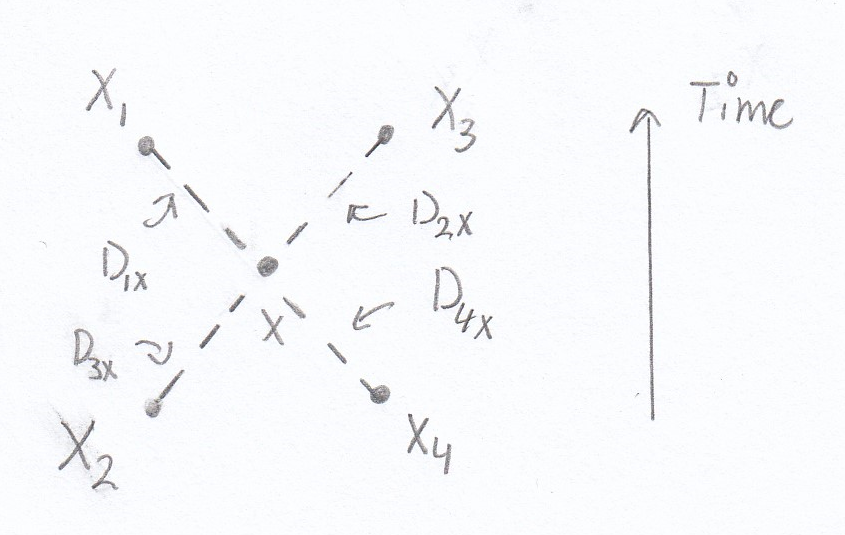
\includegraphics[width=0.5\textwidth]{figures/scal1}
		\end{figure}
		The factor of $4!$ cancels the factor of $\frac{1}{4!}$ from the Hamiltonian. Hereby, the I can write the LSZ reduction formula
		\begin{equation}
			\begin{split}
				&\frac{i}{p'_1-m^2}\frac{i}{p'_2-m^2}\frac{i}{p_1-m^2}\frac{i}{p_2-m^2}\braket{\vec{p'}_1\vec{p'}_2|iT|\vec{p}_1\vec{p}_2}=\int d^4x_1\int d^4x_2\int d^4x_3\int d^4x_4\\
				&\cdot e^{i(p'_1\cdot x_1+p'_2\cdot x_2-p_1\cdot x_3-p_2\cdot x_4)}(-i\lambda)\int d^4x\braket{0|T\{\phi(x_1)\phi(x_2)\phi(x_3)\phi(x_4)\phi^4(x)\}|0}\\
				&\cdot\frac{1}{\braket{0|T\{1-i\frac{\lambda}{4!}\int d^4x \phi^4\}|0}}.
			\end{split}
		\end{equation} 
		I consider
		\begin{equation}
			\begin{split}
				I&=\int d^4x_1\int d^4x_2\int d^4x_3\int d^4x_4e^{i(p'_1\cdot x_1+p'_2\cdot x_2-p_1\cdot x_3-p_2\cdot x_4)}\\
				&\qquad\cdot(-i\lambda)\int d^4x\braket{0|T\{\phi(x_1)\phi(x_2)\phi(x_3)\phi(x_4)\phi^4(x)\}|0}.
			\end{split}
		\end{equation}  
		To evaluate the integral I define $y_i=x_i-x$. Hereby $i(p'_1\cdot x_1+p'_2\cdot x_2-p_1\cdot x_3-p_2\cdot x_4)=i(p'_1pp'_2-p_1-p_2)\cdot x+i(p'_1\cdot y_1p'_2\cdot y_2-p_1\cdot y_3-p_2\cdot y_4)$. Using this
		\begin{equation}
			\begin{split}
				I&=-i\lambda\int d^4xe^{i(p'_1+p'_2-p_1-p_2)\cdot x}\int d^4y_1e^{ip'_1\cdot y_1}D(y_1)\int d^4y_2e^{ip'_2\cdot y_2}D(y_2)\\
				&\qquad\cdot \int d^4y_3e^{-ip_1\cdot y_3}D(y_3)\int d^4y_4e^{-ip_2\cdot y_4}D(y_4).
			\end{split}
		\end{equation}  
		Use now that $\int d^4y e^{op\cdot y}f(y)=\tilde{f}(p)$. Hereby
		\begin{equation}
			\begin{split}
				I&=-i\lambda \tilde{D}(p'_1)\tilde{D}(p'_2)\tilde{D}(p_1)\tilde{D}(p_2)\int d^4xe^{i(p'_1+p'_2-p_1-p_2)\cdot x}\\
				&=-i\lambda \tilde{D}(p'_1)\tilde{D}(p'_2)\tilde{D}(p_1)\tilde{D}(p_2)(2\pi)^4\delta^{(4)}(p'_1+p'_2-p_1-p_2)\\
				&=-i\lambda \frac{i}{p'_1-m^2}\frac{i}{p'_2-m^2}\frac{i}{p_1-m^2}\frac{i}{p_2-m^2}(2\pi)^4\delta^{(4)}(p'_1+p'_2-p_1-p_2).\\
			\end{split}
		\end{equation} 
		using $I$ in the LSZ formula the propagators now cancel, and so I find
		\begin{equation}
			\begin{split}
				\braket{\vec{p'}_1\vec{p'}_2|iT|\vec{p}_1\vec{p}_2}&=-i\lambda (2\pi)^4\delta^{(4)}(p'_1+p'_2-p_1-p_2)\frac{1}{\braket{0|T\{1-i\frac{\lambda}{4!}\int d^4x \phi^4\}|0}}.
			\end{split}
		\end{equation} 
		The denominator, ie $\braket{0|T\{1-i\frac{\lambda}{4!}\int d^4x \phi^4\}|0}$, only contribute with vacuum diagrams. this can be seen because no external fields enter. Hence, no particles will come out of this term, and only diagrams on the form shown below will enter - these are called vacuum diagrams, or bubble diagrams.
		\begin{figure}[H]
			\captionsetup{width=1\textwidth}
			\centering
			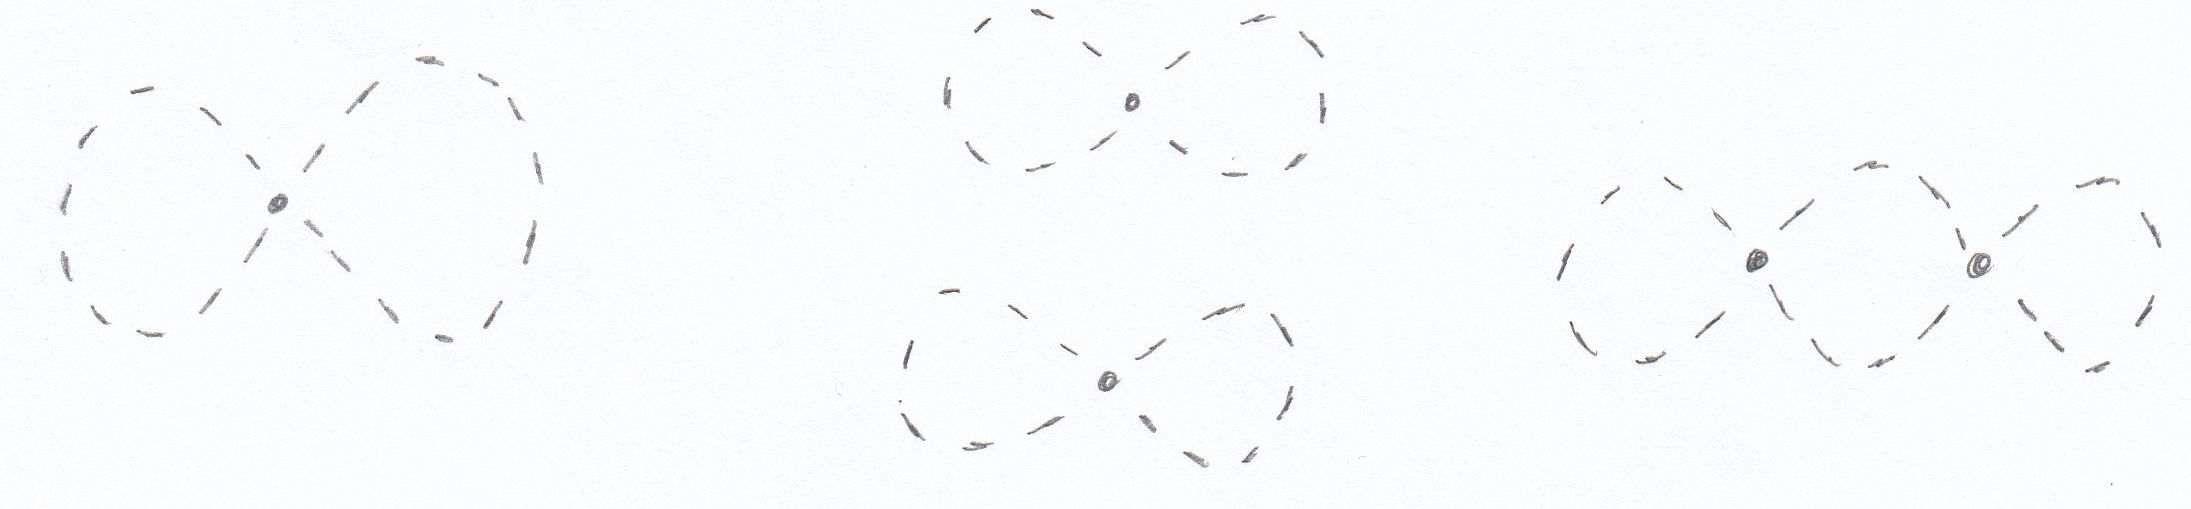
\includegraphics[width=0.6\textwidth]{figures/bub1}
		\end{figure}
		These diagrams do however also enter in the nominator, since what I have considered is only what can be measured. In practice all these vacuum diagrams can be added to the diagram describing the interaction cf.
		\begin{figure}[H]
			\captionsetup{width=1\textwidth}
			\centering
			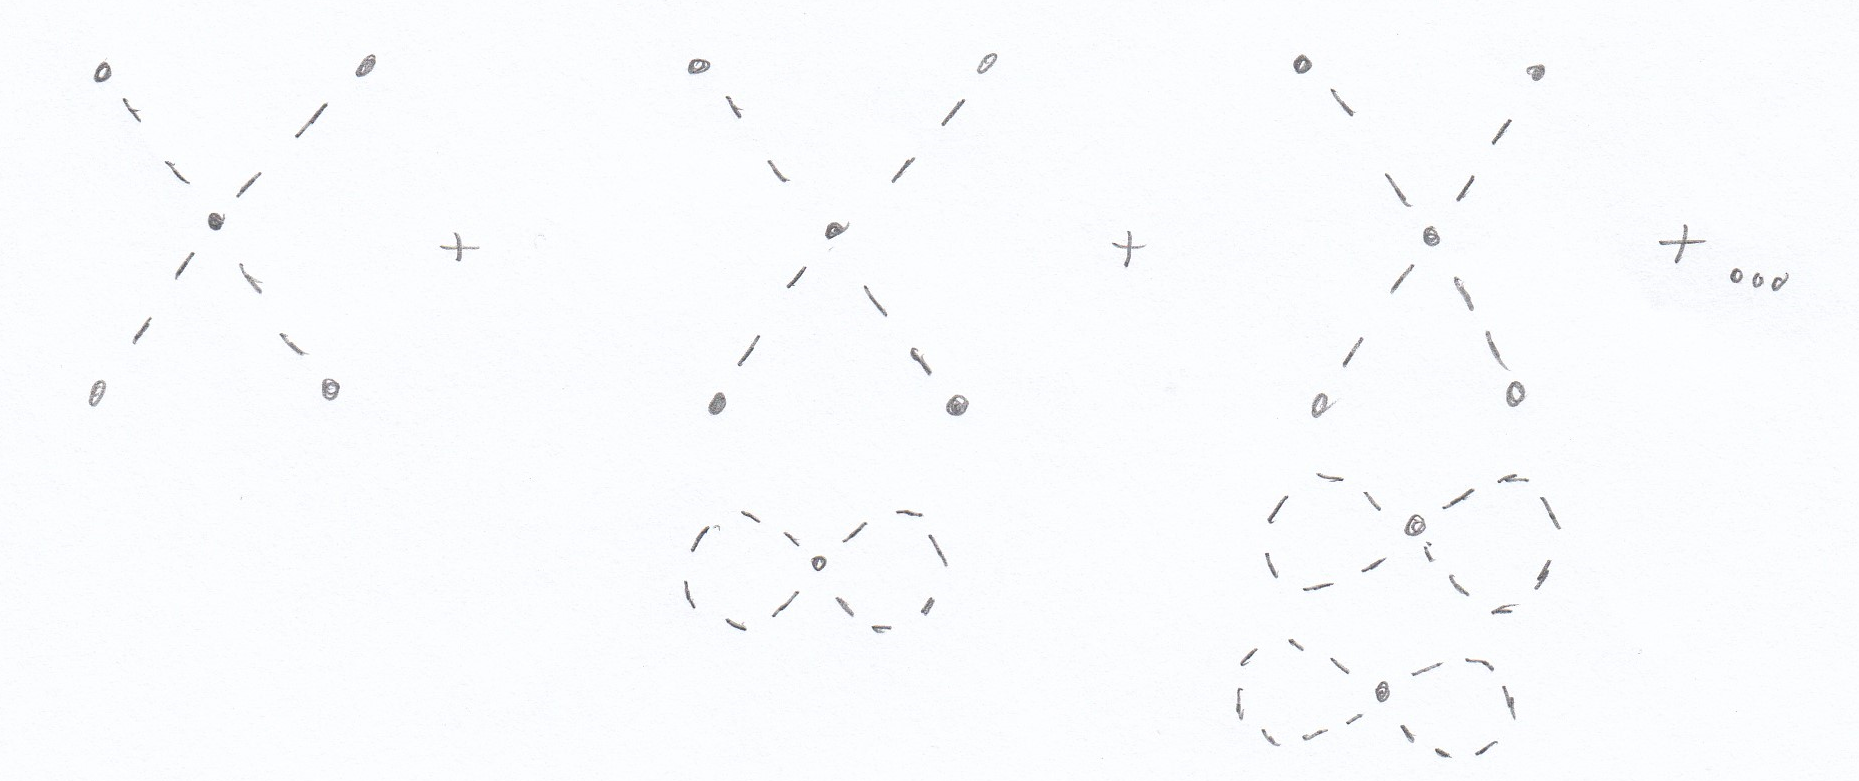
\includegraphics[width=0.6\textwidth]{figures/bub2}
		\end{figure}
		Hence, the fraction in the LSZ formula will be on the form
		\begin{figure}[H]
			\captionsetup{width=1\textwidth}
			\centering
			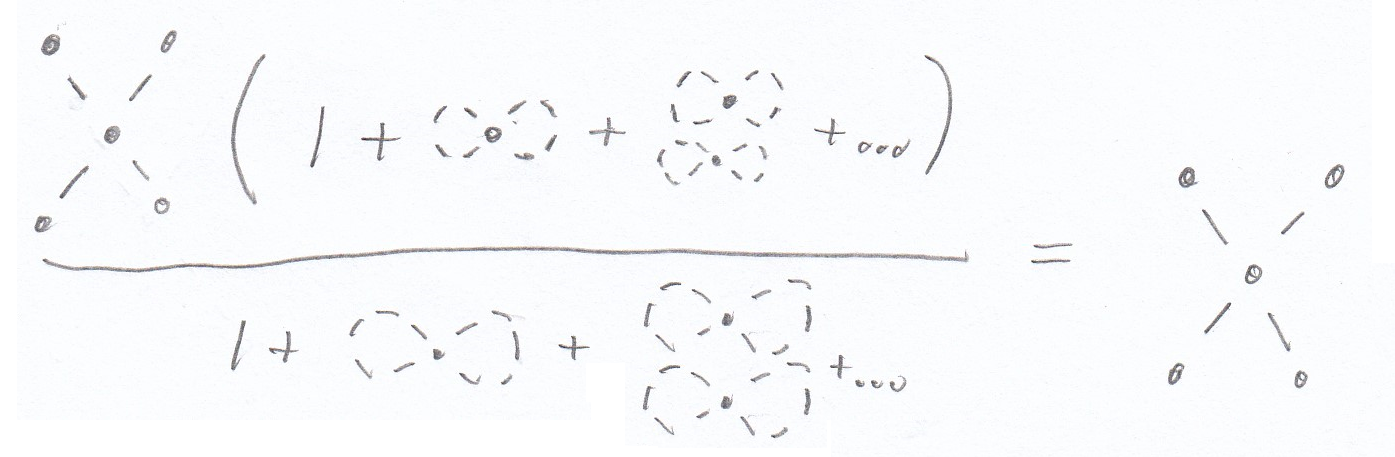
\includegraphics[width=0.6\textwidth]{figures/bub3}
		\end{figure}
		So, I can omit the vacuum diagrams in the denominator if I only consider diagrams with external particles. Hereby, I find
		\begin{equation}
			\braket{\vec{p'}_1\vec{p'}_2|iT|\vec{p}_1\vec{p}_2}=-i\lambda (2\pi)^4\delta^{(4)}(p'_1+p'_2-p_1-p_2).
		\end{equation} 
		From which it is clear that $i\mathcal{M}=-i\lambda$.
		
		\item \emph{Consider now a theory with $\mathcal{H}_I=\frac{\lambda}{3!}\phi^3$. What is the first non-vanishing term for this theory? Draw the relevant Feynman diagram.}
		
		The $\mathcal{O}(\lambda^0)$ term vanishes for the same reason that the $\mathcal{O}(\lambda^0)$ term for $\phi^4$-theory vanished; there is no interaction to zeroth order. The $\mathcal{O}(\lambda^1)$-term will however also vanish because the VEV will be on the form
		\begin{equation}
			VEV=\braket{0|T\{\phi(x_1)\phi(x_2)\phi(x_3)\phi(x_4)\phi^3(x)\}|0}.
		\end{equation} 
		Since the number of fields is uneven, not all fields can be contracted at the same time and so the VEV will be zero. Recall that this is because Wicks theorem is used to go from a time-ordered sequence of operators to a normal-ordered series. The normal-ordered terms will be zero if not all fields are contracted. Contracted fields make up a complex number that can go outside the VEV, but if there are uncontracted terms they will stay inside the VEV, and since the field is normal-ordered, the annihilation operator will be all the way to the right and annihilate onto the vacuum to make the terms vanish. Because of the previous arguments, the first non-vanishing order will be $\mathcal{O}(\lambda^2)$. Here, there will be connected terms and the number of fields will be $10$ (even), so all terms can be contracted at the same time. 
		Regarding the diagram; the previous procedure can be repeated to find the diagram, or alternatively the Feynman rules can be used. For each factor of $(-i\lambda)$ there is a vertex, where there, in this case, will be three joining lines. Hence
		\begin{figure}[H]
			\captionsetup{width=1\textwidth}
			\centering
			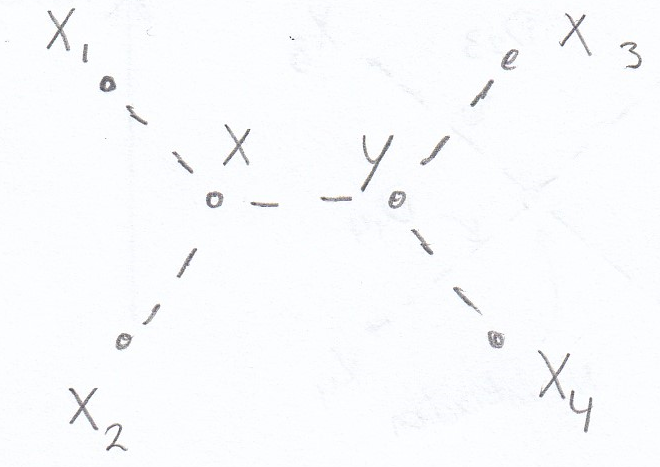
\includegraphics[width=0.4\textwidth]{figures/scal2}
		\end{figure}
		Again the vacuum diagrams will cancel. There are however other diagrams possible with two vertices:
		\begin{figure}[H]
			\captionsetup{width=1\textwidth}
			\centering
			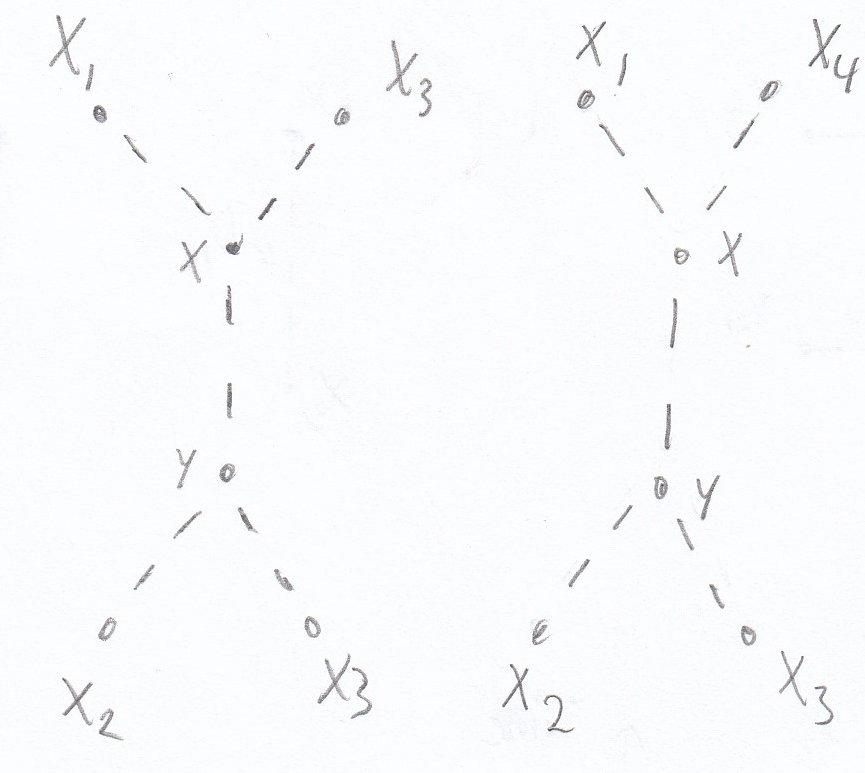
\includegraphics[width=0.3\textwidth]{figures/scal3}
		\end{figure}
		These are all the possible diagrams to leading order - Since $x_i$ has been connected to all $x_j's$. From the Feynman rules the matrix element can be found rather quickly.
		
	\end{enumerate}
	
\end{example}

\begin{example}
	\emph{Determine the lowest non-vanishing order of perturbation theory in Compton scattering.}\newline
	
	Compton scattering is an inelastic scattering between a photon and an electron,  i.e.
	\begin{equation}
		e^-(p_1)+\gamma(p_2)\Rightarrow e^-(p'_1)+\gamma(p'_2).
	\end{equation} 
	From equation \eqref{S4} the amplitude is given by
	\begin{equation}
		\begin{split}
			\mathcal{A}&=\braket{\vec{p'}_2,\vec{p'}_1|S|\vec{p}_2, \vec{p}_1}\\
			&=\braket{\vec{p'}_2,\vec{p'}_1|T\big\{1-i\int d^4x\mathcal{H}_I(x)+\frac{(-i)^2}{2!}\int d^4x_1\int d^4 x_2\mathcal{H}_I(x_2)\mathcal{H}_I(x_1)+...\big\}|\vec{p}_2, \vec{p}_1}.\\
		\end{split}
		\label{he}
	\end{equation} 
	The Hamiltonian density, $\mathcal{H}_I$, is given by
	\begin{equation}
		\mathcal{H}_{I}(x)=-|e|\bar{\psi}(x)\gamma^\mu\psi(x)A_\mu(x).
		\label{Hi}
	\end{equation} 
	The initial and final states are taken to be different and so $\braket{\vec{p'}_2,\vec{p'}_1|\vec{p}_2, \vec{p}_1}=0$. To evaluate the  time-ordered product use Wick's theorem. Wick's theorem relates the time-ordered product ($T\{...\}$) of a sequence of field operators to the normal-ordered product ($N\{...\}$). In mathematical form Wick's theorem\index{Wicks theorem} is given by
	\begin{equation}
		T\{...\}=N\{...+\text{All contractions}\}.
	\end{equation} 
	where "all contractions" refers to all contractions between the operators that the time ordering operator acts upon. The time ordering operator lists the contents with the latest entry farthest to the left whereas the normal ordering operator lists all the annihilation operators, belonging to the fields, to the right. Hence, the vacuum expectation value (VEV) of a normal ordered product is zero - since the annihilation operator acting on the vacuum is zero. Because the contraction between two field-operators is just a complex number, it can be moved outside the normal ordering operator. For this reason, only terms in which all field operators are contracted to another field operator contributes to the VEV. This leads to the important conclusion, that the number of fields must be an even number if there is to be any contribution from a given order of the perturbation theory. If the number of fields are uneven, it is not possible to contract all fields in a term, and the VEV will be zero. Because the number of fields vary with the order of the perturbation series, the leading order is the first order above zero which does not have an uneven number of fields. An important point here is that the number of fields is not the number of fields given in the interaction Hamiltonian density! There are extra fields stemming from the particle in the states involved (i.e. the initial and final states). These fields can be "pulled" out of the states (final and initial) by inserting the appropriate ladder operator, the vacuum state and a normalization factor. There are several different ways to explain, and do, this, but the point to remark here is that there appears an extra field for each final and initial particle involved in the process. Since there, for Compton scattering, are two particles, in both the initial and final state, the total number of fields is 4 plus what comes from the interaction Hamiltonian density. At $\mathcal{O}(i)$ there are three fields from the interaction Hamiltonian density, which results in seven fields in total, and so the contribution from this order vanishes. The leading order for Compton scattering is therefore $\mathcal{O}(i^2)$ (where there are 10 fields). 
	
\end{example}

\begin{example}
	\emph{Determine the invariant matrix element for Compton scattering via the Feynman rules.} \newline
	
	From considering the interaction Hamiltonian density of equation \eqref{Hi} it is clear that the vertices of QED will be of three particles; two fermions and one photon.	As seen in the previous example the leading order for Compton scattering, and QED scattering in general, is $\mathcal{O}(i^2)$. Since the number of vertices follow the order of perturbation theory there will be two vertices. Hence, the relevant diagrams will have two vertices to each of which two fermions and one photon will be attached. There are two diagrams fulfilling the requirements:
	\begin{center}
		\feynmandiagram [large, baseline=(b), vertical=a to b] {
			i1 [particle=\(\gamma\)] -- [photon, rmomentum'=\(p'_2\)] a -- [fermion, edge label'=\(p'_1\)] i2 [particle=\(e^{-}\)],
			a -- [anti fermion,edge label=\(p_1+p_2\)] b,
			f1 [particle=\(\gamma\)] -- [photon, momentum=\(p_2\)] b -- [anti fermion,edge label=\(p_1\)] f2 [particle=\(e^{-}\)],
		}; \qquad
		\feynmandiagram [large ,baseline=(b), horizontal=a to b] {
			i1 [particle=\(\gamma\)] -- [photon, momentum'=\(p_2\)] a -- [fermion,edge label'=\(p'_1\)] i2 [particle=\(e^{-}\)],
			a -- [anti fermion ,edge label=\(p_1-p'_2\)] b,
			f1 [particle=\(e^{-}\)] -- [fermion, edge label=\(p_1\)] b -- [photon,, momentum=\(p'_2\)] f2 [particle=\(\gamma\)],
		};
	\end{center}
	where the direction of time is upwards. In order to write down the invariant matrix element from the Feynman diagrams, use the following procedure; at each side of the propagator is go towards the fermion current and use the feynman rules, then insert the propagator and go towards the fermion current on the other side of the propagator. Naming the vertices in the process means
	\begin{equation}
		\begin{split}
			i\mathcal{M}_{vertical}&=\bar{u}^{s'}(\vec{p'}_1)(-iQ\gamma^\mu)\epsilon^{(\lambda')*}_{\mu}(\vec{p'}_2)\frac{i(\slashed p_1+\slashed p_2+m)}{(p_1+p_2)^2-m^2}\epsilon^{(\lambda)}_{\rho}(\vec{p}_2)(-iQ\gamma^\rho)
			u^s(\vec{p}_1)\\
			&=-i|e|^2\epsilon^{(\lambda')*}_{\mu}(\vec{p'}_2)\epsilon^{(\lambda)}_{\rho}(\vec{p}_2)\frac{\bar{u}^{s'}(\vec{p'}_1)\gamma^\mu(\slashed p_1+\slashed p_2+m)\gamma^\rho u^s(\vec{p}_1)}{(p_1+p_2)^2-m^2},
		\end{split}
		\label{M1}
	\end{equation} 
	\begin{equation}
		\begin{split}
			i\mathcal{M}_{horizontal}&=\bar{u}^{s'}(\vec{p'}_1)(-iQ\gamma^\mu)\epsilon^{(\lambda)}_{\mu}(\vec{p}_2)\frac{i(\slashed p_1-\slashed p'_2+m)}{(p_1-p'_2)^2-m^2}\epsilon^{(\lambda')*}_{\rho}(\vec{p'}_2)(-iQ\gamma^\rho)
			u^s(\vec{p}_1)\\
			&=-i|e|^2\epsilon^{(\lambda)}_{\mu}(\vec{p}_2)\epsilon^{(\lambda')*}_{\rho}(\vec{p'}_2)\frac{\bar{u}^{s'}(\vec{p'}_1)\gamma^\mu(\slashed p_1-\slashed p'_2+m)\gamma^\rho
				u^s(\vec{p}_1)}{(p_1-p'_2)^2-m^2}.
		\end{split}
		\label{M2}
	\end{equation} 
	
\end{example}


\begin{example}
	\emph{Determine the invariant matrix element for Compton scattering in position space.}\newline
	
	Position space refers to the analog of the LSZ formula. However, instead of re-deriving the LSZ formula for QED it is convenient to use a slightly different approach. Using that the lowest non-vanishing order for QED is $\mathcal{O}(i^2)$, alongside the fact that if the zeroth order is neglected in the expansion of the $S$-matrix; $\mathcal{A}\Rightarrow \braket{\dots'|iT|\dots}$, equation \eqref{he} can be written viz
	\begin{equation}
		\begin{split}
			\braket{\vec{p'}_2,\vec{p'}_1|iT|\vec{p}_2, \vec{p}_1}&=\frac{(i)^2|e|^2}{2!}\int d^4x_1\int d^4 x_2\braket{\vec{p'}_2,\vec{p'}_1|T\big\{\mathcal{H}_I(x_2)\mathcal{H}_I(x_1)\}|\vec{p}_2,\vec{p}_1},\\
		\end{split}
		\label{t1}
	\end{equation} 
	where
	\begin{equation}
		\mathcal{H}_I(x_2)\mathcal{H}_I(x_1)=\bar{\psi}(x_1)\gamma^\mu\psi(x_1)A_\mu(x_1)\bar{\psi}(x_2)\gamma^\nu\psi(x_2)A_\nu(x_2).
	\end{equation} 
	To evaluate equation \ref{t1} use Wick's theorem\index{Wicks theorem}. From Wick's theorem the time-ordering of a product of field operators, sandwiched between two states, can be written as the normal ordered product of all possible contractions between the field operators. To determine which terms should enter the sum, use the definitions of the different contractions
	\begin{equation}
		\begin{split}
			&\contraction{0}{\psi}{(x_1)}{\psi}
			\psi(x_1)\psi(x_2)=0 \\
			&\contraction{0}{\bar{\psi}}{(x_1)}{\bar{\psi}}
			\bar{\psi}(x_1)\bar{\psi}(x_2)=0\\
			&\contraction{0}{\psi}{(x_1)}{\bar{\psi}}
			\psi(x_1)\bar{\psi}(x_2)=iS_F(x_1-x_2)=\int\frac{d^4q}{(2\pi)^4}\frac{i(\slashed q+m)e^{-iq\cdot(x_1-x_2)}}{q^2-m^2}\\
			&\contraction{0}{\psi}{(x_i)}{\vec{p}_1}
			\psi(x_i)\ket{\vec{p}_1}\,\,=\int\frac{d^3q}{(2\pi)^3}\frac{1}{\sqrt{2E_{\vec{q}}}}\sum_{s'}\big(u^{s'}(\vec{q})e^{-iq\cdot x_i}a^{s'}_{\vec{q}}+v^{s'}(\vec{q})e^{iq\cdot x_i}b^{s'\dagger}_{\vec{q}}\big)\sqrt{2E_{\vec{p}_1}}\,a^{s\dagger}_{\vec{p}_1}\ket{0}\\
			&\qquad\qquad=\int\frac{d^3q}{(2\pi)^3}\frac{1}{\sqrt{2E_{\vec{q}}}}\sum_{s'}u^{s'}(\vec{q})e^{-iq\cdot x_i}a^{s'}_{\vec{q}}\sqrt{2E_{\vec{p}_1}}\,a^{s\dagger}_{\vec{p}_1}\ket{0}\\
			&\qquad\qquad=\int\frac{d^3q}{(2\pi)^3}\frac{\sqrt{2E_{\vec{p}_1}}}{\sqrt{2E_{\vec{q}}}}\sum_{s'}u^{s'}(\vec{q})e^{-iq\cdot x_i}\big(a^{s\dagger}_{\vec{p}_1}a^{s'}_{\vec{q}}+(2\pi)^3\delta^{(3)}(\vec{q}-\vec{p}_1)\delta_{s,s'}\big)\ket{0}\\
			&\qquad\qquad=u^{s}(\vec{p}_1)e^{-ip_1\cdot x_i}\ket{0}=\text{fermion, initial state}.
		\end{split}
	\end{equation} 
	From similar calculations
	\begin{equation}
		\contraction{0}{\psi}{(x_i)}{\vec{p}_1}
		\bar{\psi}(x_i)\ket{\vec{p}_1}=\bar{v}^s(p)e^{-ip\cdot x}\ket{0}=\text{anti fermion, initial state}.
	\end{equation} 
	In the case of the bra-contractions the other field operator is used
	\begin{equation}
		\begin{split}
			\contraction{0}{\vec{p'}_1}{\psi}{(x}
			\bra{\vec{p'}_1}\psi(x_i)&=\bra{0}b^{s}_{\vec{p'}_1}\sqrt{2E_{\vec{p'}_1}}\int\frac{d^3q}{(2\pi)^3}\frac{1}{\sqrt{2E_{\vec{q}}}}\sum_{s'}\big(u^{s'}(\vec{q})e^{-iq\cdot x_i}a^{s'}_{\vec{q}}+v^{s'}(\vec{q})e^{iq\cdot x_i}b^{s'\dagger}_{\vec{q}}\big)\\
			&=\int\frac{d^3q}{(2\pi)^3}\frac{\sqrt{2E_{\vec{p'}_1}}}{\sqrt{2E_{\vec{q}}}}\sum_{s'}\bra{0}b^{s}_{\vec{p'}}b^{s'\dagger}_{\vec{q}}v^{s'}(\vec{q})e^{iq\cdot x_i}\\
			&=\int\frac{d^3q}{(2\pi)^3}\frac{\sqrt{2E_{\vec{p'}_1}}}{\sqrt{2E_{\vec{q}}}}\sum_{s'}v^{s'}(\vec{q})e^{iq\cdot x_i}\bra{0}\big(b^{s'\dagger}_{\vec{q}}b^{s}_{\vec{p'}}+(2\pi)^3\delta^{(3)}(\vec{q}-\vec{p'}_1)\delta_{s,s'})\big)\\
			&=\bra{0}v^{s'}(\vec{p'}_1)e^{ip'_1\cdot x_i}=\text{anti fermion, final state}.
		\end{split}
	\end{equation} 
	Similarly
	\begin{equation}
		\contraction{0}{\vec{p'}_1}{\psi}{(x_i)}
		\bra{\vec{p'}_1}\bar{\psi}(x_i)=\bra{0}\bar{u}^{s'}(\vec{p'}_1)e^{ip'_1\cdot x_i}=\text{fermion, final state}.
	\end{equation} 
	Lastly, for the photons the possible contractions are
	\begin{equation}
		\begin{split}
			\contraction{0}{\psi}{(x_i),}{\vec{p}}
			A_\mu(x_i)\ket{\vec{p}_2}&=\int\frac{d^3q}{(2\pi)^3}\frac{1}{\sqrt{2E_{\vec{q}}}}\sum_{r}\big(\varepsilon^{r}_\mu(\vec{q})e^{-iq\cdot x_i}a^{r}_{\vec{q}}+\varepsilon^{r*}_\mu(\vec{q})e^{iq\cdot x_i}a^{r\dagger}_{\vec{q}}\big)\sqrt{2E_{\vec{p}_2}}\,a^{s\dagger}_{\vec{p}_2}\ket{0}\\
			&=\int\frac{d^3q}{(2\pi)^3}\frac{\sqrt{2E_{\vec{k}}}}{\sqrt{2E_{\vec{q}}}}\sum_{r}\varepsilon^{r}_\mu(\vec{q})e^{-iq\cdot x_i}a^{r}_{\vec{q}}\,a^{s\dagger}_{\vec{p}_2}\ket{0}\\
			&=\int\frac{d^3q}{(2\pi)^3}\frac{\sqrt{2E_{\vec{p}_2}}}{\sqrt{2E_{\vec{q}}}}\sum_{r}\varepsilon^{r}_\mu(\vec{q})e^{-iq\cdot x_i}\big(a^{s\dagger}_{\vec{k}}\,a^{r}_{\vec{q}}+(2\pi)^3\delta^{(3)}(\vec{q}-\vec{p}_2)\delta_{s,r}\big)\ket{0}\\
			&=\varepsilon_\mu^r(\vec{p}_2) e^{-ip_2\cdot x_i}\ket{0}.\\
		\end{split}
	\end{equation} 	
	Likewise
	\begin{equation}
		\begin{split}
			\contraction{0}{\vec{p'}}{\psi}{(x}
			\bra{\vec{p'_2}}A_\mu(x_i)=\bra{0}\varepsilon_\mu^{r'*}(\vec{p'}_2) e^{ip'_2\cdot x_i}.\\
		\end{split}
	\end{equation} 
	With the contractions defined as above Wick's theorem can be used to significantly simplify equation \ref{t1}. From Wick's theorem all terms must be contracted to contribute. Further more, contractions between $A$ an the other fields are zero, just as contractions among $\psi$'s and $\bar{\psi}$'s. Hence, to contribute there must be terms on the form
	\begin{equation}
		\contraction{0}{\psi}{,,,}{\bar{\psi}}
		\psi(x_1)\bar{\psi}(x_2), \quad \contraction{0}{\psi}{,,,}{\vec{p}}
		\psi(x_i)\ket{\vec{p}}, \quad \contraction{0}{\vec{p'}}{0}{(x_i)}
		\bra{\vec{p'}}\bar{\psi}(x_i), \quad 	\contraction{0}{\vec{p'}}{\psi}{(x}
		\bra{\vec{k'}}A_\mu(x_i), \quad \contraction{0}{\psi}{(x_i),}{\vec{p}}
		A_\mu(x_i)\ket{\vec{k}}.
	\end{equation} 
	There are four terms like this. Defining $I\equiv \braket{\vec{p'}_2,\vec{p'}_1|T\big\{\mathcal{H}_I(x_2)\mathcal{H}_I(x_1)\}|\vec{p}_2,\vec{p}_1}$
	\begin{equation}
		\begin{split}
			\contraction{I=N\big\{,}{\vec{p'}}{,,,\vec{k'}|}{\bar{\psi}}
			\contraction{,,,I=N\vec{p'},\vec{k'}|\bar{\psi}(x_1)\gamma^\mu}{,,\psi(x_1)}{A_\mu(x_1)}{\bar{\psi}(x_2)}
			\contraction{,,,,,,,,,,,,,,,,,,,,,,,,,,,,,,,,,,,,,,,,,,,}{\psi(x_2)}{,A_\nu(x_2)|}{\vec{p}}
			\contraction[2ex]{,,,,,,,,,,,,}{\vec{k'}}{,,,,,,,,,,,,,}{A_\mu(x_1)}
			\contraction[2ex]{,,,,.,,,,,,,,,,,,,,,,,,,,,,,,,,,,,,,,,,,,,,,,,,,}{A_\nu(x_2)}{,,,,,,}{\vec{k}}
			I&=N\big\{\braket{\vec{p'}_1,\vec{p'}_2|\bar{\psi}(x_1)\gamma^\mu\psi(x_1)A_\mu(x_1)\bar{\psi}(x_2)\gamma^\nu\psi(x_2)A_\nu(x_2)|\vec{p}_1,\vec{p}_2}\\
			&\qquad
			\contraction{,,,,}{\vec{p'}}{,,,\vec{k'}|}{\bar{\psi}}
			\contraction{,,,,,,,,,,,,,,,,,}{\psi(x_1)}{A_\mu(x_1)}{\bar{\psi}(x_2)}
			\contraction{,,,,,,,,,,,.,,,,,,,,,,,,,,,,,,,,,,,,,,}{\psi(x_2)}{,A_\nu(x_2)|}{\vec{p}}
			\contraction[3ex]{,,,,,.,}{\vec{k'}}{,,,,,,,,,,,,,,,,,,,,,,,,,,,,,,,,,}{A_\mu(x_2)}
			\contraction[2ex]{,,,,,,,,,,,,,,,,,,,,,,}{A_\nu(x_1)}{,,,,,,,,,,,,,,,,,,,,,,,,,}{\vec{k}}
			+\braket{\vec{p'}_1,\vec{p'}_2|\bar{\psi}(x_1)\gamma^\mu\psi(x_1)A_\mu(x_1)\bar{\psi}(x_2)\gamma^\nu\psi(x_2)A_\nu(x_2)|\vec{p}_1,\vec{p}_2}\\
			&\qquad
			\contraction{,,,,}{\vec{p'}}{,,,,,.,,,,,,,,,,,,,,,,,,}{\bar{\psi}(x_2)}
			\contraction[5ex]{,,,,,,,,,}{\bar{\psi}(x_1)}{,,,,,,,,,,,,,,,,,,,,,,,,}{\psi(x_2)}
			\contraction[4ex]{,,,,,,,,,,,,,,,,,}{\psi(x_1)}{,,,,,,,,,,,,,,,,,,,,,,,,,,,,,,}{\vec{p}}
			\contraction[3ex]{,,,,,.,,}{\vec{k'}}{,,,,,,,,,,,.,,,,,,,,,,,,,,,,,,,,,,}{A_\mu(x_2)}
			\contraction[2ex]{,,,,,.,,,,,,,,,,,,,,,,,}{A_\nu(x_1)}{,,,,,,,,,,,,,,,,,,,,,,,,,}{\vec{k}}
			+\braket{\vec{p'}_1,\vec{p'}_2|\bar{\psi}(x_1)\gamma^\mu\psi(x_1)A_\mu(x_1)\bar{\psi}(x_2)\gamma^\nu\psi(x_2)A_\nu(x_2)|\vec{p}_1,\vec{p}_2}\\	
			&\qquad
			\contraction{,,,,}{\vec{p'}}{,,,,.,,,,,,,,,,,,,,,,,,,}{\bar{\psi}(x_2)}
			\contraction[3ex]{,,,,,.,,,}{\bar{\psi}(x_1)}{,,,,,,,,,,,,,,,,,,,,,,,}{\psi(x_2)}
			\contraction[2ex]{,,,,,,,,,,,,,,,,,}{\psi(x_1)}{,,,,,,,,,,,,,,,,,,,,,,,,,,,,,}{\vec{p}}
			\contraction{,,,,,,,,,,,,,,,,,,,,,,,,,,,,,,,,,,,,,,,,,,,,}{\psi(x_2)}{,,,,,}{\vec{p}}
			\contraction[4ex]{,,,.,,,,}{\vec{k'}}{,,,,,,,,,,,,,}{A_\mu(x_1)}
			+\braket{\vec{p'}_1,\vec{p'}_2|\bar{\psi}(x_1)\gamma^\mu\psi(x_1)A_\mu(x_1)\bar{\psi}(x_2)\gamma^\nu\psi(x_2)A_\nu(x_2)|\vec{p}_1,\vec{p}_2}\big\}.\\
		\end{split}
		\label{I}
	\end{equation} 
	There are two different fermion terms and two different photon terms. The two different fermion terms are in fact identical. This can be seen as follows
	\begin{equation}
		\begin{split}
			\contraction{,,,,}{\vec{p'}}{,,,,,,,,,,,,,,,,,,,,,,,,,\vec{k'}|}{\bar{\psi}}
			\contraction{.,,,,,,,,.,,,,,,,,,,,,,,,,,,,,,,,,,,,,,,,,,,,,,,,,,,,,,,,,,,,,,,,}{\vec{p'}}{,..,\vec{k'}|}{\bar{\psi}}
			N\{[\bar{\psi}(x_1)\slashed A(x_1)\psi(x_1)][\bar{\psi}(x_2)\slashed A(x_2)\psi(x_2)]\}&=(-1)^4N\{[\bar{\psi}(x_2)\slashed A(x_2)\psi(x_2)][\bar{\psi}(x_1)\slashed A(x_1)\psi(x_1)]\}\\
			&\contraction{,,,,,,,,,,,,,,,,,,}{\vec{p'}}{,,,\vec{k'}|}{\bar{\psi}}
			=N\{[\bar{\psi}(x_1)\slashed A(x_1)\psi(x_1)][\bar{\psi}(x_2)\slashed A(x_2)\psi(x_2)]\}.
		\end{split}
	\end{equation} 	
	Hereby
	\begin{equation}
		\begin{split}
			I&=2\bar{u}^{s'}(\vec{p'}_1)\gamma^\mu iS_{F}(x_1-x_2)\gamma^\nu u^s(\vec{p}_1)e^{ip'_1\cdot x_1}e^{-ip_1\cdot x_2}N\{\braket{\vec{p'}_2|A_\mu(x_1)A_\nu(x_2)|\vec{p}_2}\}.
		\end{split}
	\end{equation} 
	The $A's$ can each couple to either the initial or final state, so
	\begin{equation}
		\begin{split}
			N\{\braket{\vec{p'}_2|A_\mu(x_1)A_\nu(x_2)|\vec{p}_2}\}=\varepsilon_\mu^{r'*}(\vec{p'}_2)\varepsilon_\nu^{r}(\vec{p}_2)e^{ip'_2\cdot x_1}e^{-ip_2\cdot x_2}+\varepsilon_\nu^{r'*}(\vec{p'}_2)\varepsilon_\mu^{r}(\vec{p}_2)e^{ip'_2\cdot x_2}e^{-ip_2\cdot x_1}.
		\end{split}
	\end{equation} 
	Hereby
	\begin{footnotesize}
	 \begin{equation}
		\begin{split}
			\braket{\vec{p'}_1,\vec{p'}_2|i\hat{T}|\vec{p}_1, \vec{p}_2}&=i(i)^2|e|^2\\
			&\quad \cdot\bigg(\int d^4x_1\int d^4x_2
			\bar{u}^{s'}(\vec{p'}_1)\gamma^\mu S_{F}(x_1-x_2)\gamma^\nu u^s(\vec{p}_1)e^{ip'_1 x_1}e^{-ip_1 x_2}\varepsilon_\mu^{r'*}(\vec{p'}_2)\varepsilon_\nu^{r}(\vec{p}_2)e^{ip'_2 x_1}e^{-ip_2 x_2}\\
			&\quad\quad\quad+\int d^4x_1\int d^4x_2
			\bar{u}^{s'}(\vec{p'}_1)\gamma^\mu S_{F}(x_1-x_2)\gamma^\nu u^s(\vec{p}_1)e^{ip'_1 x_1}e^{-ip_1x_2}
			\varepsilon_\nu^{r'*}(\vec{p'}_2)\varepsilon_\mu^{r}(\vec{p}_2)e^{ip'_2x_2}e^{-ip_2 x_1}\bigg)\\
			&\equiv-i|e|^2\sum_{i=1}^{2}T_i.
		\end{split}
		\label{t2}
	\end{equation} 
\end{footnotesize}	
	Considering each of the terms
	\begin{footnotesize}
	 \begin{equation}
		\begin{split}
			&T_1=\int d^4x_1\int d^4
			\bar{u}^{s'}(\vec{p'}_1)\gamma^\mu S_{F}(x_1-x_2)\gamma^\nu u^s(\vec{p}_1)e^{ip'_1 x_1}e^{-ip_1 x_2}\varepsilon_\mu^{r'*}(\vec{p'}_2)\varepsilon_\nu^{r}(\vec{p}_2)e^{ip'_2 x_1}e^{-ip_2 x_2}\\
			&\quad=\int \frac{d^4q}{(2\pi)^4}
			\bar{u}^{s'}(\vec{p'}_1)\gamma^\mu \frac{\slashed q+m}{q^2-m^2}\gamma^\nu u^s(\vec{p}_1)\varepsilon_\mu^{r'*}(\vec{p'}_2)\varepsilon_\nu^{r}(\vec{p}_2)
			\underbrace{\int d^4x_1
				e^{ip'_2\cdot x_1}e^{ip'_1 x_1}e^{-iq x_1}}_{(2\pi)^4\delta^{(4)}(p'_2+p'_1-q)}
			\underbrace{\int d^4x_2
				e^{-ip_2 x_2}
				e^{-ip_1x_2}e^{iq x_2}}_{(2\pi)^4\delta^{(4)}(p_2+p_1-q)}\\
			&\quad=(2\pi)^4\delta^{(4)}(p'_2+p'_1-p_1-p_2)\bar{u}^{s'}(\vec{p'}_1)\gamma^\mu \frac{\slashed p_1+\slashed p_2+m}{(p_1+p_2)^2-m^2}\gamma^\nu u^s(\vec{p}_1)\varepsilon_\mu^{r'*}(\vec{p'}_2)\varepsilon_\nu^{r}(\vec{p}_2),\\
			&T_2=\int d^4x_1\int d^4x_2
			\bar{u}^{s'}(\vec{p'}_1)\gamma^\mu S_{F}(x_1-x_2)\gamma^\nu u^s(\vec{p}_1)e^{ip'_1 x_1}e^{-ip_1 x_2}
			\varepsilon_\nu^{r'*}(\vec{p'}_2)\varepsilon_\mu^{r}(\vec{p}_2)e^{ip'_2 x_2}e^{-ip_2 x_1}\\
			&\quad=\int \frac{d^4q}{(2\pi)^4}
			\bar{u}^{s'}(\vec{p'}_1)\gamma^\mu \frac{\slashed q+m}{q^2-m^2}\gamma^\nu u^s(\vec{p}_1)
			\varepsilon_\nu^{r'*}(\vec{p'}_2)\varepsilon_\mu^{r}(\vec{p}_2)
			\underbrace{\int d^4x_1
				e^{ip'_1 x_1}e^{-ip_2 x_1}e^{-iqx_1}}_{(2\pi)^4\delta^{(4)}(p'_1-p_2-q)}\underbrace{\int d^4x_2e^{-ip_1 x_2}
				e^{ip'_2 x_2}e^{iq x_2}}_{(2\pi)^4\delta^{(4)}(p_1-p'_2-q)}\\
			&\quad=(2\pi)^4\delta^{(4)}(p'_2+p'_1-p_1-p_2)\bar{u}^{s'}(\vec{p'}_1)\gamma^\mu \frac{\slashed p_1-\slashed p'_2+m}{(p'_1-p'_2)^2-m^2}\gamma^\nu u^s(\vec{p}_1)
			\varepsilon_\nu^{r'*}(\vec{p'}_2)\varepsilon_\mu^{r}(\vec{p}_2).
		\end{split}
		\label{t3}
	\end{equation}
	\end{footnotesize} 
	By combining equations \eqref{t2} and \eqref{t3}
	\begin{footnotesize}
	 \begin{equation}
		\begin{split}
			\braket{\vec{p'}_1,\vec{p'}_2|i\hat{T}|\vec{p}_1, \vec{p}_2}&=-i(2\pi)^4\delta^{(4)}(p'_2+p'_1-p_1-p_2)|e|^2\varepsilon_\nu^{r'*}(\vec{p'}_2)\varepsilon_\mu^{r}(\vec{p}_2)\\
			&\quad\cdot\bigg(\bar{u}^{s'}(\vec{p'}_1)\gamma^\mu \frac{\slashed p_1+\slashed p_2+m}{(p_1+p_2)^2-m^2}\gamma^\nu u^s(\vec{p}_1)+\bar{u}^{s'}(\vec{p'}_1)\gamma^\nu \frac{\slashed p_1-\slashed p'_2+m}{(p_1-p'_2)^2-m^2}\gamma^\mu u^s(\vec{p}_1)\bigg),
		\end{split}
		\label{t4}
	\end{equation}
	\end{footnotesize} 
	where the dummy indices ($\mu,\nu$) have been relabeled on the $\gamma's$ on the second term in order to factorize the $\epsilon's$. From equation \eqref{t4}
	 \begin{equation}
		\begin{split}
			i\mathcal{M}&=-i|e|^2\varepsilon_\nu^{r'*}(\vec{p'}_2)\varepsilon_\mu^{r}(\vec{p}_2)\\
			&\qquad\cdot\bigg(\bar{u}^{s'}(\vec{p'}_1)\gamma^\mu \frac{\slashed p_1+\slashed p_2+m}{(p_1+p_2)^2-m^2}\gamma^\nu u^s(\vec{p}_1)+\bar{u}^{s'}(\vec{p'}_1)\gamma^\nu \frac{\slashed p_1-\slashed p'_2+m}{(p_1-p'_2)^2-m^2}\gamma^\mu u^s(\vec{p}_1)\bigg).
		\end{split}
		\label{M3}
	\end{equation} 
	By comparison between equation \eqref{M3}, \eqref{M2} and \eqref{M1} it is clear that the same result is obtained as in the previous example where the invariant matrix element was written directly from the Feynman rules of QED.
	
\end{example}

\section{Effective field theory}
\index{Scattering, meson}
\index{Scattering, hadron}
Particle physics often consider scattering events between hadrons and mesons. The issue with such composite particles is that the amplitude written in terms of the Feynman rules does not apply unless the particles considered are free. Quarks confined in hadrons and mesons are not free (the majority of the hadron mass is made up of the gluon field produced by the quark) and further more; the underlying theory describing the behavior of the quarks (QCD) is non-perturbative. In such cases the Feynman rules cannot be used and as such the position space approach is used. It goes as follows; the interaction (the states evolve via the interaction Hamiltonian density, $\mathcal{H}_I$, which in turn is read off from the interacting part of the interaction Lagrangian density, $\mathcal{L}_I$) Lagrangian density is related to the amplitude for a scattering by using the definition of $S$ from equation \eqref{S} alongside equation \eqref{S1} through \eqref{S4}. Taking the states to be more general, eg. $\ket{p_1, A}$ for a particle scattering of a nucleus. $p_1$ denotes the momentum of the scattered particle whereas $A$ denotes the more complex state of the nucleus (eg. with momentum, spin,...) and using equation \eqref{S} in equation \eqref{S1} (and expanding the exponential)
\begin{equation}
	\begin{split}
		\mathcal{A}&=\braket{f|S|i}\\
		&=\braket{f|i}-i\int d^4x\braket{f|\mathcal{H}_I(x)|i}+\mathcal{O}(i^2),
	\end{split}
	\label{S5}
\end{equation} 
where $i$ denotes the initial state, $f$ denotes the final state and $\mathcal{H}_I(x)$ is the interaction Hamiltonian in the interaction picture. From equation \eqref{S4}
\begin{equation}
	\begin{split}
		\mathcal{A}&=\braket{f|i}+(2\pi)^4\delta^{(4)}(\Sigma p'-\Sigma p)i\mathcal{M}.
	\end{split}
	\label{S6}
\end{equation} 
By equating equation \eqref{S5} and \eqref{S6}
\begin{equation}
	(2\pi)^4\delta^{(4)}(\Sigma p'-\Sigma p)i\mathcal{M}=-i\int d^4x\braket{f|\mathcal{H}_I(x)|i} +\mathcal{O}(i^2).
	\label{S7}
\end{equation} 
Taking $p^\mu$ to be the space-time translation operator, the interaction Hamiltonian density can be written as follows
\begin{equation}
	\mathcal{H}_I(x)=e^{ipx}\mathcal{H}_{I}(0)e^{-ipx}.
	\label{S8}
\end{equation} 
By applying equation \eqref{S8} in equation \eqref{S7}
\begin{equation}
	\begin{split}
		(2\pi)^4\delta^{(4)}(\Sigma p'-\Sigma p)\mathcal{M}&=-\int d^4x\braket{f|e^{ipx}\mathcal{H}_I(0)e^{-ipx}|i}+\mathcal{O}(i^2)\\
		&=-\int d^4xe^{-i(\Sigma p-\Sigma p')x} \braket{f|\mathcal{H}_I(0)|i}+\mathcal{O}(i^2)\\
		&=-(2\pi)^4\delta^{(4)}(\Sigma p'-\Sigma p) \braket{f|\mathcal{H}_I(0)|i}+\mathcal{O}(i^2).\\
	\end{split}
	\label{S9}
\end{equation} 
From equation \eqref{S9} it is clear that
\begin{equation}
	\mathcal{M}=-\braket{f|\mathcal{H}_I(0)|i}+\mathcal{O}(i^2).
\end{equation} 
If the interaction Lagrangian does not contain derivatives, then $-\mathcal{L}_I(0)=\mathcal{H}_I(0)$. Hereby
\begin{equation}
	\mathcal{M}=\braket{f|\mathcal{L}_I(0)|i}+\mathcal{O}(i^2).
	\label{S10}
\end{equation} 
$\mathcal{L}_I(0)$ can then be described by an effective Lagrangian density\index{Fermi Lagrangian}. An effective Lagrangian density is a Lagrangian density that is proportional to product of the two currents of the interaction. The effective Lagrangian density is valid only in the limit in which the momentum of the mediator squared goes to zero, i.e. $q^2\Rightarrow 0$. In the case of a massless mediator, eg. a photon, this would make the propagator diverge, so this approach is only valid in the case of a massive propagator, eg. the low energy limit of the electroweak theory. The usefulness of this approach is when scatterings between constituent particles is considered. 

\begin{example}
	For example WIMP-nucleus scattering. In this case the WIMP will scatter with the quarks inside the nucleons in the nucleus. Hence, the particle are not free and the usual Feynman rules do not apply. However, an effective Lagrangian density can be written viz
	\begin{equation}
		\mathcal{L}_I(0)\simeq \sum_{x,y}\sum_q \frac{C_q^{(xy)}}{\Lambda^2} [\bar{\chi}\Gamma_x\chi]\,[\bar{q}\Gamma_yq],
	\end{equation} 
	where $q$ denotes quarks, $\Lambda^2$ is the mediator mass squared, $\Gamma_i$ denote the possible objects that makes the term a Lorentz scalar and $C_q^{(xy)}\sim g^2$ is related to the square of the coupling. From this effective Lagrangian density, the invariant matrix element is given by
	\begin{equation}
		\mathcal{M}\simeq \sum_{x,y}\sum_q\frac{C_q^{(xy)}}{\Lambda^2} \braket{\chi_f|\bar{\chi}\Gamma_x\chi|\chi_i}\braket{A_f|\bar{q}\Gamma_yq|A_i},
	\end{equation} 
	where $A$ denotes the nucleus states. From this expression the matrix elements can, through a considerable amount of work, be determined.
	
\end{example}
\begin{example}
	As an illustrative example, consider the decay of a neutral kaon, $K^0$, into negative pion, $\pi^-$, a neutrino, $\nu_l$, and its corresponding lepton, $l^{+}$, i.e. $K^0\Rightarrow \pi^-+l^++\nu_l$ (see the Feynman diagram below).
	\begin{figure}[H]
		\captionsetup{width=1\textwidth}
		\centering
		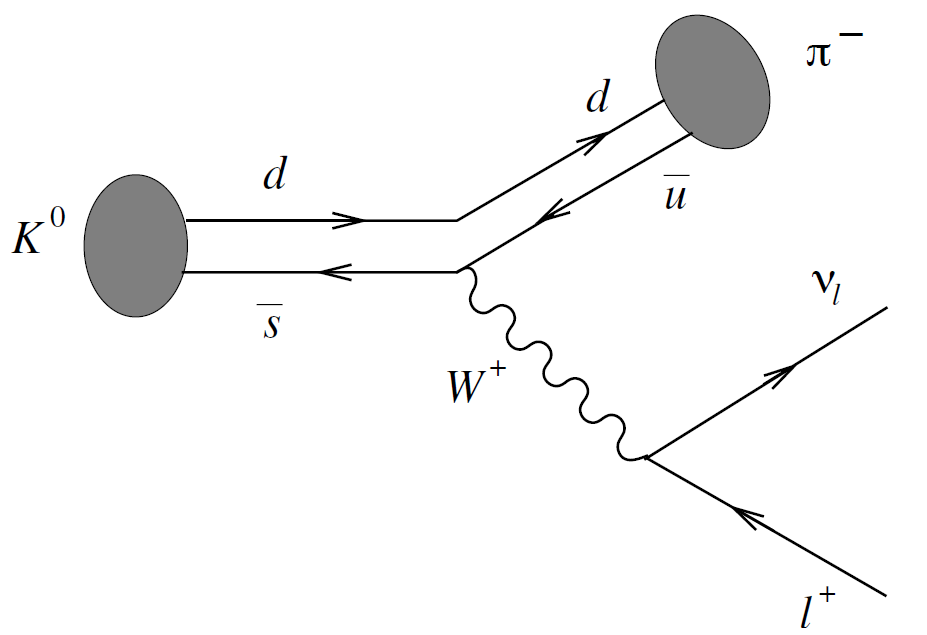
\includegraphics[width=0.4\textwidth]{figures/feyn1}
	\end{figure}
	In this case the states read $\ket{i}=\ket{\nu_l=0}\otimes \ket{l^{+}=0}\otimes\ket{K^0}$ and $\bra{f}=\bra{\pi^-}\otimes \bra{l^+}\otimes \bra{\nu_l}$. The effective Lagrangian density for the decay is given by
	\begin{equation}
		\mathcal{L}_I(0)=-\frac{G_fsin(\theta_C)}{\sqrt{2}}\bar{\nu}_l\gamma_\mu(1-\gamma^5)l\bar{s}\gamma^\mu(1-\gamma^5)u.
		\label{L2}
	\end{equation} 
	Equation \eqref{L2} is a Fermi Lagrangian density since the mediator is integrated out. It is however not an effective Lagrangian density since the coupling is specified. From equation \eqref{L2}
	\begin{equation}
		\begin{split}
			\mathcal{M}&=-\frac{G_fsin(\theta_C)}{\sqrt{2}}\bra{f}\bar{\nu}_l\gamma_\mu(1-\gamma^5)l\bar{s}\gamma^\mu(1-\gamma^5)u\ket{i}+\mathcal{O}(i^2)\\
			&=-\frac{G_fsin(\theta_C)}{\sqrt{2}}\bra{\nu_l}\bar{\nu}_l\ket{0}\gamma_\mu(1-\gamma^5)\bra{l^+}l\ket{0}\bra{\pi^-}\bar{s}\gamma^\mu(1-\gamma^5)u\ket{K^0}+\mathcal{O}(i^2)\\
			&=-\frac{G_fsin(\theta_C)}{\sqrt{2}}\bar{u}(\nu_l)\gamma_\mu(1-\gamma^5)v(l^+)\bra{\pi^-}\bar{s}\gamma^\mu(1-\gamma^5)u\ket{K^0}+\mathcal{O}(i^2),\\
		\end{split}
		\label{S12}
	\end{equation}   
	where it is understood that all matrix elements are evaluated at $x=0$. The matrix element of the quark current, i.e. the second operator, cannot be evaluated directly like the matrix element of the leptonic matrix element, i.e. the first operator. Instead the matrix element of the second operator can be parameterized in terms of form factors. The parameterization is determined by Lorentz invariance and depends in general on the specific process under consideration. The procedure to determine the amplitude in processes involving composite particles is however clear; use the Fermi Lagrangian and determine the quark-matrix elements via parameterization.
\end{example}